\documentclass[11pt,]{article}
\usepackage{lmodern}
\usepackage{amssymb,amsmath}
\usepackage{ifxetex,ifluatex}
\usepackage{fixltx2e} % provides \textsubscript
\ifnum 0\ifxetex 1\fi\ifluatex 1\fi=0 % if pdftex
  \usepackage[T1]{fontenc}
  \usepackage[utf8]{inputenc}
\else % if luatex or xelatex
  \ifxetex
    \usepackage{mathspec}
  \else
    \usepackage{fontspec}
  \fi
  \defaultfontfeatures{Ligatures=TeX,Scale=MatchLowercase}
\fi
% use upquote if available, for straight quotes in verbatim environments
\IfFileExists{upquote.sty}{\usepackage{upquote}}{}
% use microtype if available
\IfFileExists{microtype.sty}{%
\usepackage{microtype}
\UseMicrotypeSet[protrusion]{basicmath} % disable protrusion for tt fonts
}{}
\usepackage[margin=1.0in]{geometry}
\usepackage{hyperref}
\hypersetup{unicode=true,
            pdftitle={Who are ASM Journals? A Gender-based Analysis},
            pdfborder={0 0 0},
            breaklinks=true}
\urlstyle{same}  % don't use monospace font for urls
\usepackage{longtable,booktabs}
\usepackage{graphicx,grffile}
\makeatletter
\def\maxwidth{\ifdim\Gin@nat@width>\linewidth\linewidth\else\Gin@nat@width\fi}
\def\maxheight{\ifdim\Gin@nat@height>\textheight\textheight\else\Gin@nat@height\fi}
\makeatother
% Scale images if necessary, so that they will not overflow the page
% margins by default, and it is still possible to overwrite the defaults
% using explicit options in \includegraphics[width, height, ...]{}
\setkeys{Gin}{width=\maxwidth,height=\maxheight,keepaspectratio}
\IfFileExists{parskip.sty}{%
\usepackage{parskip}
}{% else
\setlength{\parindent}{0pt}
\setlength{\parskip}{6pt plus 2pt minus 1pt}
}
\setlength{\emergencystretch}{3em}  % prevent overfull lines
\providecommand{\tightlist}{%
  \setlength{\itemsep}{0pt}\setlength{\parskip}{0pt}}
\setcounter{secnumdepth}{0}
% Redefines (sub)paragraphs to behave more like sections
\ifx\paragraph\undefined\else
\let\oldparagraph\paragraph
\renewcommand{\paragraph}[1]{\oldparagraph{#1}\mbox{}}
\fi
\ifx\subparagraph\undefined\else
\let\oldsubparagraph\subparagraph
\renewcommand{\subparagraph}[1]{\oldsubparagraph{#1}\mbox{}}
\fi

%%% Use protect on footnotes to avoid problems with footnotes in titles
\let\rmarkdownfootnote\footnote%
\def\footnote{\protect\rmarkdownfootnote}

%%% Change title format to be more compact
\usepackage{titling}

% Create subtitle command for use in maketitle
\newcommand{\subtitle}[1]{
  \posttitle{
    \begin{center}\large#1\end{center}
    }
}

\setlength{\droptitle}{-2em}

  \title{\textbf{Who are ASM Journals? A Gender-based Analysis}}
    \pretitle{\vspace{\droptitle}\centering\huge}
  \posttitle{\par}
    \author{}
    \preauthor{}\postauthor{}
    \date{}
    \predate{}\postdate{}
  
\usepackage{booktabs}
\usepackage{longtable}
\usepackage{array}
\usepackage{multirow}
\usepackage[table]{xcolor}
\usepackage{wrapfig}
\usepackage{float}
\usepackage{colortbl}
\usepackage{pdflscape}
\usepackage{tabu}
\usepackage{threeparttable}
\usepackage{threeparttablex}
\usepackage[normalem]{ulem}
\usepackage{makecell}
\usepackage{caption}

\usepackage{helvet} % Helvetica font
\renewcommand*\familydefault{\sfdefault} % Use the sans serif version of the font
\usepackage[T1]{fontenc}

\usepackage[none]{hyphenat}

\usepackage{setspace}
\doublespacing
\setlength{\parskip}{1em}

\usepackage{lineno}

\usepackage{pdfpages}
\floatplacement{figure}{H} % Keep the figure up top of the page

\begin{document}
\maketitle

\vspace{35mm}

Running title: A gender-based analysis of ASM journals

\vspace{35mm}

Ada K. Hagan\(^{*1}\), Begüm D. Topçuoğlu\({^1}\), Mia Gregory\({^1}\),
Hazel Barton\({^2}\), Patrick D. Schloss\textsuperscript{1\(\dagger\)}

\vspace{40mm}

\(\dagger\) To whom correspondence should be addressed:
\href{mailto:pschloss@umich.edu}{\nolinkurl{pschloss@umich.edu}}

*Present address: Alliance SciComm \& Consulting, Linden, MI

1. Department of Microbiology and Immunology, University of Michigan,
Ann Arbor, MI

2. Department of Biology, University of Akron, Akron, OH

\newpage

\linenumbers

\subsection{Abstract}\label{abstract}

Despite 50\% of biology Ph.D.~graduates being women, the number of women
that advance in academia decreases at each level (e.g.~from graduate to
post-doctorate to tenure-track). Recently, scientific societies and
publishers have begun examining internal submissions data to evaluate
representation of, or bias against, women in their peer review
processes; however, representation and attitudes differ by scientific
field and no studies to-date seem to have investigated academic
publishing in the field of microbiology. Using manuscripts submitted
between January 2012 and August 2018 to the 15 journals published by the
American Society for Microbiology (ASM), we describe the representation
of women at ASM journals and the outcomes of their manuscripts. We find
that senior women authors at ASM journals are underrepresented compared
to global and society estimates of microbiology researchers.
Additionally, manuscripts submitted by corresponding authors that were
women received more negative outcomes (e.g., editorial rejections,
reviewer recommendations, and decisions after review) than those
submitted by men. These negative outcomes were somewhat mediated by
whether or not the corresponding author was based in the US or not, and
by the institution for US-based authors. Nonetheless, the pattern for
women corresponding authors to receive more negative outcomes on their
submitted manuscripts indicates a pattern of gender-influenced editorial
decisions. We conclude with suggestions to improve the representation
of, and decrease bias against, women.

\subsection{Importance}\label{importance}

Barriers in science and academia have prevented women from becoming
researchers and experts that are viewed equivalent to their colleagues
who are men. We evaluated the participation and success of women
researchers at ASM journals to better understand their success in the
field of microbiology. We found that women are underrepresented as
expert scientists at ASM journals. This is due to a combination of both
low submissions from senior women authors and increased rejection rates
for women compared to men.

\subsection{Introduction}\label{introduction}

Evidence has accumulated over the decades that academic research has a
representation problem. While at least 50\% of biology Ph.D.~graduates
are women, the number of women in postdoctoral positions and
tenure-track positions are less than 40 and 30\%, respectively (1).
There have been many proposed reasons for these disparities, which
include biases in training and hiring, the impact of children on career
trajectories, a lack of support for primary caregivers, a lack of
recognition, lower perceived competency, and less productivity as
measured by research publications (1--7). These issues do not act
independent of one another, instead they accumulate for both individuals
and the community, much as advantages do (8, 9). Accordingly, addressing
these issues necessitates multi-level approaches from all institutions
and members of the scientific community.

Scientific societies play an integral role in the formation and
maintenance of scientific communities. They host conferences that
provide forums for knowledge exchange, networking, and opportunities for
increased visibility as a researcher. Scientific societies also
frequently publish the most reputable journals in their field,
facilitating the peer review process to vet new research submissions
(10). Recently, scientific societies and publishers have begun examining
internal submissions data to evaluate representation of, and bias
against, women in their peer review processes. The American Geological
Union found that while the acceptance rate of women-authored
publications was greater than publications authored by men, women
submitted fewer manuscripts than men and were used as reviewers only
20\% of the time (11), a factor influenced by the gender of the editor
(12). Several studies have concluded that there is no significant bias
against papers authored by women (12--17). Recent reports of manuscript
outcomes at publishers for ecology and evolution, physics, and chemistry
journals have found that women-authored papers are less likely to have
positive peer reviews and outcomes (18--21).

The representation of women scientists and gender attitudes differ by
scientific field and no studies to-date have investigated academic
publishing in the field of microbiology. The American Society for
Microbiology (ASM) is one of the largest life science societies, with an
average membership of 41,000 since 1990. In its mission statement, the
ASM notes that it is ``an inclusive organization, engaging with and
responding to the needs of its diverse constituencies'' and pledges to
``address all members' needs through development and assessment of
programs and services.'' One of these services is the publication of
microbiology research through a suite of research and review journals.
Between January 2012 and August 2018, ASM published 25,818 original
research papers across 15 different journals: \emph{Antimicrobial Agents
and Chemotherapy} (AAC), \emph{Applied and Environmental Microbiology}
(AEM), \emph{Clinical and Vaccine Immunology} (CVI), \emph{Clinical
Microbiology Reviews} (CMR), \emph{Eukaryotic Cell} (EC),
\emph{Infection and Immunity} (IAI), \emph{Journal of Bacteriology}
(JB), \emph{Journal of Clinical Microbiology} (JCM), \emph{Journal of
Virology} (JVI), \emph{mBio}, \emph{Microbiology and Molecular Biology
Reviews} (MMBR), \emph{Genome Announcements} (GA, now \emph{Microbiology
Resource Annoucements}), \emph{Molecular and Cellular Biology} (MCB),
\emph{mSphere}, and \emph{mSystems}. The goal of this research study was
to describe the population of ASM journals through the gender-based
representation of authors, reviewers, and editors and the associated
peer review outcomes.

\subsection{Results}\label{results}

Over 100,000 manuscript records were obtained for the period between
January 2012 and August 2018 (Fig. 1). Each of these were evaluated by
editors and/or reviewers, leading to multiple possible outcomes.
Manuscripts may be immediately rejected by editors instead of being sent
to peer review, often due to issues of scope or quality. These were
defined as editorial rejections and identified as manuscripts rejected
without review. Alternately, editors send many manuscripts out for
review by two or more experts in the field from a list of potential
reviewers suggested by the authors and/or editors. Reviewers give
feedback to the authors and editor, who decides whether the manuscript
in question should be accepted, rejected, or sent back for revision. At
ASM journals, manuscripts with suggested revisions that are expected to
take more than 30 days are rejected, but generally encouraged to
resubmit. If resubmitted, the authors are asked to note the previous
(related) manuscript and the re-submission is assigned a new manuscript
number. Multiple related manuscripts were tracked together by generating
a unique grouped manuscript number based on the recorded related
manuscript numbers. This grouped manuscript number served dual purposes
of tracking a single manuscript through multiple rejections and avoiding
duplicate counts of authors for a single manuscript. After eliminating
non-primary research manuscripts and linking records for resubmitted
manuscripts, there were 79,189 unique manuscripts processed (Fig. 1).

We inferred genders of both peer review gatekeepers (e.g.,
editor-in-chief, editors, reviewers) and authors on the manuscripts
evaluated during this time period using a social media-informed
classification algorithm with stringent criteria and validation process
(Supp Text). We recognize that biological sex (male/female) is not
always equivalent to the gender that an individual presents as
(man/woman), which is also distinct from the gender(s) that an
individual may self-identify as. For the purposes of this manuscript, we
choose to focus on the presenting gender based on first names (and
appearance for editors), as this information is what reviewers and
editors also have available. Among the individuals inferred to be either
men or women, the sensitivity and specificity of our method were 0.97
when validated against a curated set of authors and editors (Supp Text).
In addition to identifying journal participants as men or women, this
method of gender inference resulted in a category of individuals whose
gender could not be reliably inferred (i.e., unknown). We included those
individuals whose names did not allow a high degree of confidence for
gender inference in the ``unknown'' category of our analysis, which is
shown in many of the plots depicting representation of the population.
These individuals were not included in the comparison of manuscript
outcomes.

\textbf{Men dominate as gatekeepers and senior authors.} We first
evaluated the representation of men and women who were gatekeepers
during the study period. Each journal is led by an editor-in-chief (EIC)
who manages journal scope and quality standards through a board of
editors with field expertise that, in turn, handle the peer review
process. There were 17 EICs, 17.6\% of which were women. Two journals,
EC and CVI were retired during the period under study. Four years before
retirement, the leadership of CVI transferred from a man EIC to a woman,
while JVI has had a woman as EIC since 2012. The total number of editors
at all ASM journals combined over the duration of our study (senior
editors and editors pooled) was 1015, 28.8\% of which were women.

Over 40\% of both men and women editors were from US-based R1
institutions, defined as doctoral-granting universities with very high
research activity. Non-US institutions, and U.S. medical schools or
research institutions supplyed the next largest proportions of editors
(Fig. 2A)(22). Since 2012, there was a slow trend toward equivalent
gender representation among editors (Fig. 2B). The trends for each
journal varied considerably, though most had slow trends toward parity
(Fig. S1). CVI and \emph{mSphere} were the only ASM journals to have
accomplished equivalent representation of both genders, with CVI having
a greater proportion of women editors than men before it was retired. EC
was the only journal with an increasing parity gap.

Altogether, 30439 reviewers submitted reviews and 24.6\% were inferred
to be women. The greatest proportion of reviewers (over 50\% of all
groups) came from non-US institutions, while R1 institutions supplied
the next largest cohort of reviewers (Fig. 2C). The proportions of each
gender were steady among reviewers at ASM journals (Fig. 2D) and
representative of both the suggested reviewers at all journals combined,
and the actual reviewer proportions at most journals (Fig. S2).

\textbf{Editorial workloads were not proportionate.} Across all journals
combined, men handled a slightly greater proportion of manuscripts than
women, relative to their respective editorial representations (Fig. 3A).
This trend was present at most individual journals with varying degrees
of difference between workload and representation (Fig. S1). For
instance, at \emph{mSphere}, both workload and proportions were
identical; however, CVI, \emph{mBio}, and JVI each had periods at which
the workload for women editors was much higher than their
representation, with corresponding decreases in the workload of men. In
the years preceding its retirement, the representation of women at CVI
increased, decreasing the gap in editorial workload. However,
representation and relative workloads for men and women editors at JVI
have held steady over time, while the proportionate workload for women
at \emph{mBio} has increased.

The median number of manuscripts reviewed by men, women, and unknown
individuals was 2, for each group. Half of those in the men, women, or
unknown gender groups reviewed between one and 5, 4, or 3 manuscripts
each, respectively (Fig. 3B). Conversely, 44.6\% of men, 40.1\% of
women, and 48.6\% of unknown gendered reviewers reviewed only one
manuscript, suggesting that women were more likely than other groups to
review multiple manuscripts. Reviewers of all genders accepted fewer
requests to review from women editors (average of 47.8\%) than from men
(average of 53.3\%; Fig. 3C). Reviewers were also less likely to respond
to women editors than men (no response rate averages of 25.1 and 19.9\%,
respectively). Editors of both genders contacted reviewers from all
three gender groups in similar proportions, with women editors
contacting 76.4\% of suggested reviewers and men contacting 74.1\%
(median of the percent contacted from each gender group).

\textbf{Women were underrepresented as authors.} Globally, microbiology
researchers are 60\% men and 40\% women (23). In September 2018, 38.4\%
of ASM members who reported their gender were women. We wanted to
determine if these proportions were similar for authors at ASM journals
and to understand the distribution of each gender among submitted
manuscripts and published papers. We began by describing author
institutions by gender. Over 60\% of submitting senior authors (last or
corresponding) were from non-US institutions, followed by about 20\%
from R1 institutions (Fig. 4A). The proportions of all men and women
authors at ASM decreased over time at equivalent rates, as the
proportion of unknown gendered authors increased; the ratio of men to
women authors was 4 to 3 (i.e., 57\% men; Fig. 4B).

In the field of microbiology, order of authorship on manuscripts signals
the type and magnitude of contributions to the finished product. First
and last authorships are the most prestigious. First authors are
generally trainees (e.g., students or post-docs) or early career
researchers responsible for the bulk of the project, while last authors
are lead investigators that supply conceptual guidance and resources to
complete the project. Middle authors are generally responsible for
technical analyses and methods. Any author can also be a corresponding
author, which we identified as the individual responsible for
communicating with publishing staff during peer review (as opposed to an
author to whom readers direct questions).

The proportion of manuscripts submitted with men and women as first
authors remained constant at 29.1 and 30.7\%, respectively (Fig. 4C,
dashed). The proportions of their published papers were nearly identical
at 33.1\% for men and 33.8\% for women. The proportion of submitted
manuscripts with men corresponding authors remained steady at an average
of 41.6\% and the proportion with women corresponding authors was at
23.4\% (Fig. 4D, dashed). Both men and women corresponding authors had a
greater proportion of papers published than manuscripts submitted.
Accordingly, manuscripts with corresponding authors of unknown gender
were rejected at a higher rate than their submission. The difference
between submitted manuscripts and published papers was 8.2\% where men
were corresponding authors, but only 0.9\% where women were
corresponding authors. This trend was similar for middle and last
authors (Fig. S3).

Of 38594 multi-author manuscripts submitted by men corresponding
authors, 23.5\% had zero women authors. In contrast, 7253 (36.3\%) of
manuscripts submitted by women corresponding authors had a majority of
the authors as women, exceeding those submitted by men corresponding
authors in both the number (3247) and percent (8.4) of submissions.
Additionally, the proportion of women authors decreased as the number of
authors increased (Fig. S4). Men submitted 225 single-authored
manuscripts while women submitted 69 single-authored manuscripts.

Using the metadata described, we hypothesized that we would be able to
predict the inferred gender of the corresponding author. We trained a
logistic regression model to predict the inferred gender of the
corresponding author using the following variables: whether the
corresponding author's institution was in the U.S., the total number of
authors, the proportion of authors that were women, whether the paper
was published, the gender of senior editors and editors, the number of
revisions, and whether the manuscript was editorially rejected at any
point. We measured the model's performance using the area under the
receiver operating characteristic curve (AUROC). The AUROC value is a
predictive performance metric that ranges from 0.0, where the model's
predictions are completely wrong, to 1.0, where the model perfectly
distinguishes between outcomes. A value of 0.5 indicates the model did
not perform better than random. The median AUROC value of our model to
predict the corresponding author's inferred gender was 0.7. The variable
with the largest weight (i.e., the most predictive value), in our model
was the proportion of women authors. These results indicate that
manuscript submission data was capable of predicting the inferred gender
of the corresponding author, but that prediction was primarily driven by
the percentage of authors that were inferred to be women.

As described above, first authors were slightly more likely to be women
(30.7\%W vs 29.1\%M), but corresponding authors were significantly more
likely to be men (23.44\%W vs 41.59\%M). A concern is that if authors
are not retained to transition from junior to senior status, they are
also left out of the gatekeeping roles. Since authorship conventions
indicate that last and corresponding authors are typically senior
authors, we combined both first and middle authors into the ``junior''
author role and tracked individuals through the possible roles at ASM
journals. There were 75451 women who participated as junior authors
(first/middle) at ASM journals. Of those junior authors who were women,
8.2\% also participated as senior authors (last/corresponding), 8.9\%
were potential reviewers and 5.4\% participated as reviewers. 0.2\% of
women junior authors were also editors at ASM journals. For men, there
were a total of 83727 junior authors, where 13.6\% also participated as
senior authors, 16.7\% were potential reviewers, and 11.1\% actually
reviewed. 0.7\% of men junior authors were also editors at ASM journals.
Overall, women were half as likely to move to senior author or reviewer
roles, and 30\% as likely to be an editor than men.

\textbf{Manuscripts submitted by women have more negative outcomes than
those submitted by men.} To better understand the differences between
published and submitted proportions for men and women authors (Fig. 4CD,
Fig. S3), we compared the rejection rates of men and women at each
author stage (first, middle, corresponding, and last). Middle authors
were rejected at equivalent rates for men and women (a 0 percentage
point difference across all journals). However, manuscripts with senior
women authors were rejected more frequently than those authored by men
with -1.64 and -0.92 percentage point differences for corresponding and
last authors, respectively (Fig. 5A, vertical line). There were several
instances where the overall trend of overperformance by men was repeated
at the journal level (e.g., JB, \emph{mSytesms}, \emph{mBio}). The
greatest differences were observed when comparing the outcome of
corresponding authors by gender, so we used this sub-population to
further examine the difference in manuscript acceptance and rejection
rates between men and women.

We next compared the rejection rates for men and women corresponding
authors after two bottlenecks, initial review by the editor and the
first round of peer review. Manuscripts authored by women were
editorially rejected as much as 12 percentage points more often than
those authored by men (Fig. 5B). The difference at all ASM journals
combined was -3.8 percentage points (vertical line). MCB and \emph{mBio}
had the most extreme percentage point differences. Manuscripts authored
by men and women were equally likely to be accepted after the first
round of review (Fig. 5C, right panel). However, women-authored papers
were rejected (left panel) more often while men-authored papers were
more often given revision (center panel) decisions. The differences for
rejection and revision decisions after review were -5.6 and 5.6
percentage points, respectively (Fig. 5C, vertical lines). JB, AAC, and
MCB had the most extreme differences for rejection and revision
decisions. Percentage point differences were not correlated with journal
prestige as measured by impact factors (R\({^2}\) = -0.022, P = 0.787).

In addition to manuscript decisions, other disparate outcomes may occur
during the peer review process (24). To determine whether accepted
women-authored manuscripts spent more time between being submitted and
being ready for publication, we compared the number of revisions, days
spent in the ASM peer review system, and the number of days from
submission to being ready for publication to those authored by men.
Manuscripts authored by women took slightly longer (from submission to
ready for publication) than those by men at some journals
(\emph{mSphere}, \emph{mBio}, \emph{mSystems}, CVI, JB, JCM, AEM)
despite spending similar amounts of time in the ASM journal peer review
system (Fig. S5), and having the same median number of revisions prior
to acceptance (Median = 2, IQR = 0).

To understand how a gatekeeper's (editor/reviewer) gender influenced
decisions (e.g., Fig. 5C), we grouped editor decisions and reviewer
suggestions according to the gatekeeper's gender. Both men and women
editors rejected proportionally more women-authored papers, however the
difference in decisions were more extreme for men-edited manuscripts
(Fig. 6A). Reviewers were more likely to suggest rejection for
women-authored manuscripts as compared to men, although a minimal
difference in revise recommendations was observed (Fig. 6B). Both men
and women reviewers recommended rejection more often for women-authored
manuscripts although men recommended acceptance and revision more often
for men-authored manuscripts than women did (Fig. 6C).

To evaluate if gender played a role in manuscript editorial decisions,
we trained a L2-regularized logistic regression model to predict whether
a manuscript was reviewed (i.e.~editorially rejected or not). We used
the inferred genders of the senior editor, editor, and corresponding
author, as well as the proportion of authors that were women as
variables to train the model. The median AUROC value was 0.61, which
indicated that editorial decisions were not random, however, the AUROC
value was relatively low indicating that there are factors other than
those included in our model that influence editorial decisions.

\textbf{Multiple factors contribute to the overperformance of men.} The
association between gender and manuscript decision could be attributed
to gender bias by journal gatekeepers, however, there are other types of
bias that may contribute to, or obscure, overt gender bias; for
instance, a recent evaluation of peer-review outcomes at \emph{eLife}
found evidence of preference for research submitted by authors from a
gatekeeper's own country or region (18). Other studies have documented
prestige bias, where men are over-represented in more prestigious (i.e.,
more respected and competent) programs (25). It is therefore possible,
that what seems to be gender bias could be geographic or prestige bias
interacting with the increased proportion of women submitting from
outside the US or at lower prestige institutions (e.g., the highest rate
of submissions from women were at low research institutions, 37\%; Fig.
4A).

To quantify how these factors affect manuscript decisions, we next
looked at the outcome of manuscripts submitted only by corresponding
authors at US institutions, because these institutions represented the
majority of manuscripts and could be classified by the Carnegie
Foundation (22). For reference, the proportion of manuscripts submitted
from US institutions by women was 31\% versus 36\% from women at non-US
institutions. When only considering US-based authors, the difference for
editorial rejections increased from -3.8 to -1.4 percentage points (Fig.
7A). The difference in decisions after review for US-based authors
mirrored those seen for all corresponding authors at the journal level
(Fig. 7B). The over-representation of women in rejection decisions
increased from -5.6 to -4.4 percentage points, and the
over-representation of men in revise only decisions decreased from 5.6
to 4.2 (Fig. 7B). The difference in the rate of accept decisions changed
from -1.4 to 0.2 percentage points after restricting the analysis to
US-based authors. These results suggest that the country of origin
(i.e., US versus not) accounted for some of the observed gender bias,
particularly for editorial rejections.

To address institution-based prestige bias, we split the US-based
corresponding authors according to the type of institution they were
affiliated with (based on Carnegie classification) and re-evaluated the
differences for men and women (22). Editorial rejections occurred most
often for women from medical schools or institutes, followed by those
from R2 institutions: 32\% and 28\% of manuscripts from each institution
were submitted by women, respectively (Fig. 7C, Fig. S6A). This
difference in the editorial rejections of corresponding authors from
medical schools or institutes was spread across most ASM journals, while
the editorial rejection of papers submitted from women at R2
institutions was driven primarily by submissions to JCM. Evaluating the
difference in acceptance rates by institution and gender mirrored that
of editorial rejections for some journals, where submissions from men
outperformed submissions from women. For instance, manuscripts submitted
by men from medical schools or institutes were accepted up to 20
percentage points more than those submitted by women (Fig. S6B).

To evaluate if these factors affect manuscript decisions, we trained a
L2-regularized regression model to predict if a manuscript was
editorially rejected or not, using the variables: origin (US vs non),
institution (US institution type), number of authors, proportion of
authors that were women, and the inferred genders of both gatekeepers
and corresponding authors. The model had a median AUROC value of 0.67,
which indicated a non-random interaction between these factors and
editorial decisions. Manuscripts from authors at U.S. ``other''
institutions, men EICs, men that were corresponding authors from
``other'' U.S. institutions, and women from medical schools and
institutes were more associated with editorial rejections (Fig. S6C).
Conversely, manuscripts from R1 institutions, authors from the U.S.,
EICs that were women, and the number of authors were more likely to be
associated with review (Fig. S6C). These results confirm that the
country of origin and class of institutions impact decisions in a
non-random manner, though not as much as gender.

A final factor we considered was whether the type of research pursued by
men as opposed to women may impact manuscript outcomes. Black women
philosophers and physicists have described the devaluation of
non-traditional sub-disciplines in their fields (26--28). While
originally focused on bias against Black women---the intersection of two
historically marginalized identities---the concept that researchers in
an established core field might be skeptical of less established, or
non-traditional, sub-field research likely applies elsewhere. A bias
against sub-fields in a gendered context has recently been observed in
the biomedical sciences, where NIH proposals focusing on women's
reproductive health were the least likely to be funded (29). To explore
the phenomenon in ASM journals, we looked at the editorial rejection
rates of all manuscripts (regardless of origin or institution) for each
research category at the five largest ASM journals: AAC, AEM, IAI, JVI,
and JCM. Together, these journals account for 47\% of the manuscripts
analyzed in this study across 55 categories.

The number of submissions in each category ranged from 1 (FDA Approval
at AAC) to 2952 (Bacteriology at JCM) while the acceptance rates varied
from 29.4\% (Chemistry:Biosynthesis at AAC) to 71.3\% (Structure and
Assembly at JVI) (Table 1). We argud that the number of submissions to
each category could help indicate core versus periphery subfields,
(i.e., core subfields would have more submissions than periphery
subfields) and based on the literature to-date, we expected that
periphery subfields might have a higher participation of women. Women
submitted on average 35.3\% of the manuscripts to each category. Fifteen
of the categories had submissions from more than 40\% women, and at
least 20\% of submissions to each category was from women (Table 1).
There was not a correlation between the proportion of women authors and
the number of submissions (R\({^2}\) = -0.0177, P = 0.779) to each
category. Nor was there a correlation between the proportion of women
authors and the category acceptance rate (R\({^2}\) = 0.041, P = 0.078).
These data suggest that there is not a relationship between the
participation of women and either the number of submissions or the
acceptance rate of categories in our dataset.

We next looked at the differences of performance for men and women in
each category at two decision points: editorial rejection and rejection
after the first review. Each journal focuses on a different facet of
microbiology or immunology, making the results difficult to compare
directly. However, the pattern of increased rejection rates for women
over men was maintained across most categories with some categories
displaying major differences in gendered performance (Fig. S7). For
instance, the Biologic Response Modifier (e.g., immunotherapy)
sub-category at AAC, had extreme differences for both editorial
rejections and rejections after review, about -30 and -40 percentage
points, respectively. While that category had a relatively low number of
submissions (N = 44), 43\% were from women (Fig. S7A). One category,
Mycology, was represented at two journals, AEM and JCM. At both
journals, men overperformed relative to women in this category. At AEM,
there were 73 Mycology submissions, 44\% from women authors that had a
difference of almost -20 for editorial rejection outcomes and -10 for
rejections after review (Fig. S7B). JCM had 587 Mycology submissions
with a submission rate of 39\% from women authors (Fig. S7D).
Differences between outcomes were almost -10 for editorial rejections
and -12 for rejections after review at JCM.

Because of these extreme percentage point differences in categories with
high women authorship, we next asked if the number of women
participating in a particular category was related to manuscript
outcomes. There was no correlation between the difference in editorial
rejection by category and the percent of women that were either authors
(R\({^2}\) = -0.003, P = 0.363) or editors (R\({^2}\) = -0.018, P =
0.765). The percent of women authors and percent of women editors in
journal categories did not correlate either (R\({^2}\) = -0.007, P =
0.682), which is likely related to the underrepresentation of women
editors in categories dominated by women authors (e.g., Epidemiology).
These data suggest the possibility of persistent (e.g., by editors and
reviewers) bias against women in particular fields (e.g., Mycology),
though it does not seem to relate to either the number of submissions or
participation of women in those subfields.

\subsection{Discussion}\label{discussion}

We described the representation of men and women at ASM journals between
January 2012 and August 2018 and compared editorial outcomes according
to the authors' gender. Women were consistently under-represented (30\%
or less in all levels of the peer review process) excluding first
authors, where women represented about 50\% of authors where we could
infer a gender (Figs. 2 and 4). Women and men editors had proportionate
workloads across all ASM journals combined, but those workloads were
disproportionate at the journal level and the overburdened gender varied
according to the journal (Figs. 3 and S1). Additionally, manuscripts
submitted by corresponding authors that were women, received more
negative outcomes (e.g., editorial rejections), than those submitted by
men (Figs. 5 and 6). These negative outcomes were somewhat mediated by
whether the corresponding author was based in the US, the type of
institution for US-based authors, and the research category (Figs. 7 and
S7). However, the trend for women corresponding authors to receive more
negative outcomes held, indicating a pattern of gender-influenced
editorial decisions regardless of journal prestige (as determined by
impact factor). Together, these data indicate a persistent bias against
senior women microbiologists who participate in ASM journals.

The proportion of women as first authors is higher than data obtained
globally and from self-reported ASM membership data, which was higher
than the proportion of senior women authors at ASM journals. Only half
as many women who were junior authors at ASM journals were also senior
authors when compared to men, and the representation of women decreased
as the prestige (e.g., reviewer, editor) increased. These trends are
consistent with representation of senior women in academic biological
sciences and the observation that women are more likely to leave
academia during the transition from postdoc (junior) to investigator
(senior) (30). These data indicate that microbiology (as represented by
ASM journals) is not exempt from the issues that limit the retention of
women through academic ranks.

How to define representation and determine what the leadership should
look like are recurring questions in STEM. Ideally, the representation
for men and women corresponding authors, reviewers, and editors would
reflect the number of Ph.D.s awarded (about 50\% each, when considered
on a binary spectrum). We argue that the goal should depend on the
workload and visibility of the position. Since high visibility positions
(e.g., editor, EIC) are filled by a smaller number of individuals that
are responsible for recruiting more individuals into leadership, filling
these positions should be done aspirationally (i.e., 50\% should be
women if the goal were an aspirational leadership). This allows greater
visibility for women as experts, expansion of the potential reviewer
network, and recruitment into those positions (31--33). Conversely,
lower visibility positions (e.g., reviewers) require effort from a
greater number of individuals and should thus be representational of the
field to avoid overburdening the minority population (i.e., since 23.5\%
of corresponding authors to ASM journals are women, then 20-25\% of
reviewers should be women). Balancing the workload is particularly
important given the literature indicating that women faculty have higher
institutional service loads than their counterparts who are men (34).

In contrast to institutional service, the editing workload at ASM
journals seems to be predominantly borne by men. A possible explanation
for the difference in gatekeeper representation and editor workloads is
that women are more likely to study non-traditional sub-disciplines
(26--28). Their separation from the traditional center of a field
decreases their perceived competency, which could result in research
typecasting and lower manuscript handling responsibilities. However, our
data could not confirm this phenomenon at ASM journals. Another
possibility is the increased proportion of potential reviewers that
either do not accept, or do not respond to, requests to review from
women editors. This increases the proportion of reviewers that women
editors must contact, adding additional time and work to their editorial
burdens, thus making them seem less efficient (i.e., less capable) than
men editors. Three journals, \emph{mBio}, CVI, and JVI were exceptions
with regards to editorial workloads. At these journals, the editorial
workloads of women exceeds their representation. A possible explanation
for CVI and JVI is that both of these journals have been led by women
EICs. The tendency for reviewers to reject requests to review from
editors that are women, may also extend to editors that are men; this
could result in men editors being more likely to reject requests to
handle manuscripts from EICs that are women. Our data differ from those
of Fox, Burns, and Meyer who found that the gender of the editor
influenced the gender of the contacted reviewers (12), but supports
findings that women editors contact more reviewers than men (35).

Our data also revealed some disturbing patterns in gendered authorship
that have implications for the retention of women microbiologists.
Previous research suggests that women who collaborate with other women
receive less credit for these publications than when they collaborate
with men (36), and that women are more likely to yield corresponding
authorship to colleagues that are men (19). In our linear regression
models, the number of authors on a manuscript was the largest
contributor to avoiding editorial rejections, suggesting that highly
collaborative research is preferred by editors (37). This observation
was supported by the positive correlation between citations and author
count (Fig. S6). It was concerning that when the number of authors
exceeded 30 on a manuscript (N=59), the proportion of individuals
inferred to be women was always below 51\%, despite equivalent numbers
of trainees in the biological sciences (Fig. S4). Additionally, while
women corresponding authors submitted fewer manuscripts, more of them
(both numerically and proportionally), had a majority of women
co-authors, compared to those submitted by men corresponding authors,
which supports previous findings that women are more likely to
collaborate with other women (21, 38--40). This gender-based segregation
of collaborations at ASM journals likely has had consequences in pay and
promotion for women and could be a factor in the decreased retention of
senior women. It would likely be aggravated by the under representation
of women as corresponding authors, which may also have negative
consequences for their careers and microbiology, since senior
authorships impact status in the field. Buckley et al., suggested that
being selected as a reviewer increases the visibility of a researcher,
which has a direct and significant impact on salary (16). Therefore, the
under representation of women as senior authors and reviewers likely
hampers their career progression and even their desire to progress,
since status in the peer review process also signals adoption of the
researcher into the scientific community (16, 41). The retention of
women is important to the progress of microbiology since less diversity
in science limits the diversity of perspectives and approaches, thus
stunting the search for knowledge.

Whether academic research journals support women has been the topic of
many papers, which note the lack of women authors publishing relative to
men in high impact journals (42--48). However, submissions data is
required to determine if the lack of representation is due to low
submissions or bias during peer review. We have shown that there is a
disparity in submissions from senior women in microbiology compared to
men, but this does not fully account for the difference in publications
by men and women corresponding authors at ASM journals (Fig. 4). When
examining manuscript outcomes, we found a consistent trend favoring
positive outcomes for manuscripts submitted by corresponding authors
that were men (Fig. 5). Manuscripts submitted by corresponding authors
who were women were editorially rejected at greater rates, and
gatekeepers of both genders favored rejection for manuscripts authored
by women. Neither geographic (i.e., US or not), institution type, nor
sub-discipline can fully account for the observed gender-based bias
(Fig. 6, Fig. 7, Fig. S6, Fig. S7). Instead, the presence of bias
favoring men over women from U.S. R1 institutions and medical schools
and institutes suggests that the bias persists, even in environments
with generally excellent resources and infrastructure for research.
Science and the peer review system select for decisions that are often
based on the assumption that scientists are objective, impartial
experts. As a result, scientists who believe themselves immune to bias
are making decisions that inherently rely on biases to speed the
process. The types of biases at play and their potential roles in peer
review are well documented (49, 50). For instance, previous studies show
that a greater burden of proof is required for women to achieve similar
competency as men and that women are less likely to self-promote (and
are penalized if they do) (6, 51, 52). These and similar biases might
train women to be more conservative in their manuscript submissions,
making our observed bias even more concerning.

Even if a gatekeeper does not know the corresponding author or their
gender, there remain ample avenues for implicit bias during peer review.
The stricter standard of competency has led women to adopt different
writing styles from men, resulting in manuscripts with increased
explanations, detail, and readability than those authored by men (24,
53). These differences in writing can act as subtle cues to the author's
gender. Additionally, significant time, funds, and staff are required to
be competitive in highly active fields, but women are often at a
disadvantage for these resources due to the cumulative affects of bias
(8, 9). As a result, corresponding authors that are women may be
spending their resources in research fields where competition impacts
are mitigated and/or on topics that are historically understudied. This
has the disadvantage of further decreasing perceived competency of these
women scientists compared to those studying core research field(s)
(26--28). Alternatively, non-traditional research may be seen as less
impactful, leading to poorer peer review outcomes (29). These
possibilities are reflected in our data, since while the number of
revisions before publication is identical for both men and women,
manuscripts authored by women have increased rejection rates and time
spent on revision. This suggests that manuscripts submitted by women
receive more involved critiques (i.e., work) from reviewers and/or their
competency to complete revisions within the prescribed 30 days is
doubted, compared to men. Women may also feel that they need to do more
to meet reviewer expectations, thus leading to longer periods between a
decision and resubmission. Finally, our data show a penalty for women
researching mycology (Fig. S7). Despite being among the most deadly
communicable diseases in 2016 (along with tuberculosis and diarrheal
diseases), mycology is an underserved, and underfunded, field in
microbiology that has historically been considered unimportant (54--56).
Microbiology would benefit from a more nuanced evaluation of sub-fields
to better understand how they interact with gender and peer review
outcomes.

A limitation to our methodology is the use of an algorithm to infer
gender from first names. This method left us with a category of unknown
gendered individuals and the gender of an individual may be interpreted
differently according to the reader (e.g., Kim is predominately a
woman's name in the U.S., but likely a man's name in other cultures).
The increase in unknown gendered authors corresponds to an increase in
submissions to ASM journals from Asian countries, particularly China.
Anecdotally, most editorial rejections are poor quality papers from
Asia. Our method had low performance on non-gendered languages from this
region (Supp Text) resulting in exclusion of many Asia-submitted
manuscripts from the decision outcome analyses, which increased our
confidence that the trends observed were gender-based. Another concern
might be the small effect size observed in many analyses. The
consistency of decisions to benefit men corresponding authors over women
across all journals included in this study, in addition to accumulated
literature to-date, confirms that this descriptive study is highly
relevant for the ASM as a society. Our findings offer opportunities to
address gendered representation in microbiology and systemic barriers in
peer review at our journals.

All parties have an opportunity and obligation to advance
underrepresented groups in science (57). We suggest that journals
develop a visible mission, vision, or other statement that commis to
equity and inclusion and includes a non-discrimination clause regarding
decisions made by editors and editors-in-chief. This non-discrimination
clause would be backed by a specific protocol for the reporting of, and
response to, instances of discrimination and harassment. Second, society
journals should begin collecting additional data from authors and
gatekeepers (e.g., race, ethnicity, gender identity, and disabilities).
Such author data should not be readily available to journal gatekeepers,
but instead kept in a dis-aggregated manner that allows for public
presentation and tracking the success of inclusive measures to maintain
accountability. Third, society journals can implement mechanisms to
explicitly provide support for women and other minority groups, reward
inclusive behavior by gatekeepers, nominate more women to leadership
positions, and recruit manuscripts from sub-fields that are more likely
to attract women and other minorities (29). Gatekeepers and authors can
help advance women (and other marginalized groups) within the peer
review system by changing how they select experts in their field. For
instance, authors can suggest more women as reviewers using
``Diversify'' resources (58), while reviewers can agree to review for
women editors more often. Editors can rely more on manuscript reference
lists and data base searches than personal knowledge to recruit
reviewers (59), and journals can improve the interactivity and
functionality of the reviewer selection software. Given the propensity
for journals to recruit editors and EiCs from within their already
biased reviewer pools, opening searches to include more scientists in
their reviewer pool and/or editors from outside the journal while
enacting more transparent processes could be a major component of
improving representation. Growing evidence suggests that representation
problems in STEM are due to retention rather than recruitment. We need
to align journal practices to foster the retention of women and other
minority groups.

Most approaches to overcoming bias focus on choices made by individuals,
such as double-blinded reviews and implicit bias training, but these
cannot fully remedy the effects of bias and may even worsen outcomes
(60, 61). Since bias (gender, geographic, prestige, or otherwise) is
partially the result of accumulated disadvantages and actions resulting
from implicit biases, a structural, system-wide approach is required.
Broadly, peer review is a nebulous process with expectations and
outcomes that vary considerably, even within a single journal. Academic
writing courses suffer similar issues and have sought to remedy them
with rubrics. When implemented correctly, rubrics can reduce bias during
evaluation and enhance the evaluation process for both the evaluator and
the evaluatee (62--65). We argue that rubrics could be implemented in
the peer review process to focus reviewer comments, clarify editorial
decisions, and improve the author experience. Such rubrics should
increase the emphasis on \textbf{solid} research, as opposed to novel or
``impactful'' research, the latter of which is a highly subjective
measure (66, 67). This might also change the overall attitude toward
replicatitive research and negative results, thus bolstering the field
through reproduciblity. We also argue that reconsidering journal scope
and expanding honorary editorial boards might help address structural
barriers of bias against women (and other minorities) in peer review.
Expanding journal scope and adding more handling editors would improve
the breadth of research published, thus providing a home for more
non-traditional and underserved research fields (the case at
\emph{mSphere} with an increased pool of editors). Implementing these
steps to decrease bias---review rubrics, increased focus on solid
research, expansion of journal scopes and editorial boards---will also
standardize competency principles for researchers at ASM journals and
improve microbiology as a whole.

This report demonstrates that although the level of bias at many ASM
journals is small, it is present. Peer review at ASM journals is not
immune to the accumulated disadvantages against women in microbiology.
However, the adaptation of women (and other marginalized groups) to bias
(e.g., area of research and communication styles), make it impossible to
address at the individual level. Instead, we must commit to changing the
fundamental structure and goals of peer review to minimize bias. We
encourage ASM journals, as well as other societies, to institute more
fair and transparent procedures and approaches of peer review. The
self-correcting nature of science is a badge that scientists wear
proudly, but no single report or action can correct the inertia of a
millenniums-old instiution. Instead, it requires the long-standing and
steady actions of many. Our findings reflect many similar reports, and
suggest concrete actions to correct the inertia of peer review at all
levels. The next step is commitment and implimentation.

\subsection{Data and Methods}\label{data-and-methods}

\textbf{Data.} All manuscripts handled by ASM journals (e.g.,
\emph{mBio}, \emph{Journal of Virology}) that received an editorial
decision between January 1, 2012 and August 31, 2018 were supplied as
XML files by ASM's publishing platform, eJP. Data were extracted from
the XML documents provided, manipulated, and visualized using R
statistical software (version 3.4.4) and relevant packages. Variables of
interest included: the manuscript number assigned to each submission,
manuscript type (e.g., full length research, erratum, editorial),
category (e.g., microbial ecology), related (i.e., previously submitted)
manuscripts, number of versions submitted, dates (e.g., submission,
decision), author data (e.g., first, last, and corresponding authorship,
total number of authors), reviewer data (e.g., recommendation, editor
decision), and personal data (names, institutions, country) of the
editors, authors, and reviewers. For this analysis, only original,
research-based manuscripts were included, e.g., long- and short-form
research articles, New-Data Letters, Observations, Opinion/Hypothesis
articles, and Fast-Track Communications. To help protect the
confidentiality of peer review, names were removed from all records, and
identifying data (e.g., manuscript numbers, days of date), were replaced
with randomized values.

\textbf{Institution classification.} To identify the communities
represented, we used Carnegie classifications to group US-based academic
institutions into R1 research (very high research activity), R2 research
(high research activity), four-year medical schools, or low research
(i.e., not R1, R2, or medical school) (22). Research institutes (e.g.,
Mayo Clinic, Cold Springs Harbor), industry (e.g., pharmaceutical), and
federal (e.g., NIH, CDC) research groups were identified using the
internet. Four-year medical schools and research institutions were
grouped together since these typically share research prestige and have
considerable resources to support research. Industry and federal
research were grouped separately. The ``Other'' category represents
uncategorized US institutions. Non-US institutions were a category on
their own.

\textbf{Gender inference.} The genderize.io API was used to infer an
individual's gender based on their given name and country where
possible. The genderize.io platform uses data gathered from social media
to infer gender based on given names with the option to include an
associated language or country to enhance the probability of successful
inference. Since all manuscripts were submitted in English, which
precludes language association for names with special characters, names
were standardized to ASCII coding (e.g., ``José'' to ``Jose''). We next
matched each individuals' country against the list of 242 country names
accepted by genderize.io. Using the GenderGuesser package for R, all
unique given names associated with an accepted country were submitted to
the genderize.io API and any names returned without an inferred value of
either male or female were resubmitted without an associated country.
The data returned include the name, inferred gender (as ``male'',
``female'', ``unknown''), the probability of correct gender inference
(ranging from 0.5 to 1.0), and the number of instances the name and
gender were associated together (1 or greater). The inferred genders of
all given names (with and without an associated country) whose
probabilities were greater or equal to a modified probability (pmod) of
0.85 were used to infer genders (man/woman) of the individuals in our
data set (Supp Text). The presenting gender (man/woman) of editors and
senior editors in our data set was inferred by hand using Google where
possible, and the algorithm was validated using both editor and
published data (Supp Text)(5).

\textbf{Manuscript outcome analysis.} To better visualize and understand
the differences in outcomes according to author gender, we calculated
the difference in percentage points between the proportion of that
outcome for men and women. To correct for the disparity in the
participation of women relative to men at ASM journals, all percentage
point comparisons were made relative to the gender and population in
question. For instance, the percentage point difference in acceptance
rates was the acceptance rate for men minus the acceptance rate for
women. A positive value indicated that men received the outcome more
often than women, whereas a negative value indicated that women
outperformed men in the given metric.

\textbf{Logistic regression models.} For the L2-regularized logistic
regression models, we established modeling pipelines for a binary
prediction task (68). First, we randomly split the data into training
and test sets so that the training set consisted of 80\% of the full
data set while the test set was composed of the remaining 20\% of the
data. To maintain the distribution of the two model outcomes found with
the full data set, we performed stratified splits. The training data was
used to build the models and the test set was used for evaluating
predictive performance. To build the models, we performed an internal
five-fold cross-validation where we tuned the cost hyper-parameter,
which determines the regularization strength where smaller values
specify stronger regularization. This internal cross-validation was
repeated 100 times. Then, we trained the full training data set with the
selected hyper-parameter values and applied the model to the held-out
data to evaluate the testing predictive performance of each model. The
data-split, hyper-parameter selection, training and testing steps were
repeated 25 times to get a reliable and robust reading of model
performance. Models were trained using the machine learning wrapper
caret package (v.6.0.81) in R (v.3.5.0).

\textbf{Code and data availability} Anonymized data and code for all
analysis steps, logistic regression pipeline, and an Rmarkdown version
of this manuscript, is available at
\url{https://github.com/SchlossLab/Hagan_Gender_mBio_2019/}

\textbf{Acknowledgements} We would like to thank Nicole Broderick and
Arturo Casadevall for providing their data set for genderize validation
and acknowledge Arianna Miles-Jay and Joshua MA Stough for their
comments.

A.K.H. was responsible for data aggregation, analysis, interpretation,
and drafting the manuscript. B.T. completed the logistic regression
models. M.G. verified editor genders. A.K.H., H.B., and P.D.S. were
involved with conceptual development. Funding and resources were
provided by P.D.S. All authors contributed to the final manuscript.
P.D.S. is Chair of ASM Journals and A.K.H. was ASM staff prior to
publication of the analysis. B.T., M.G., and H.B. report no conflict of
interest.

Funding and access to the data for this work were provided by the
American Society for Microbiology. Early drafts were read by the ASM
Journals Committee with minimal influence on content or interpretation.

\newpage

\subsection{References}\label{references}

\hypertarget{refs}{}
\hypertarget{ref-sheltzer_elite_2014}{}
1. \textbf{Sheltzer JM}, \textbf{Smith JC}. 2014. Elite male faculty in
the life sciences employ fewer women. Proceedings of the National
Academy of Sciences \textbf{111}:10107--10112.
doi:\href{https://doi.org/10.1073/pnas.1403334111}{10.1073/pnas.1403334111}.

\hypertarget{ref-moss-racusin_science_2012}{}
2. \textbf{Moss-Racusin CA}, \textbf{Dovidio JF}, \textbf{Brescoll VL},
\textbf{Graham MJ}, \textbf{Handelsman J}. 2012. Science faculty's
subtle gender biases favor male students. Proceedings of the National
Academy of Sciences \textbf{109}:16474--16479.
doi:\href{https://doi.org/10.1073/pnas.1211286109}{10.1073/pnas.1211286109}.

\hypertarget{ref-Ceci2012}{}
3. \textbf{Ceci S}, \textbf{Williams W}. 2012. When scientists choose
motherhood. American Scientist \textbf{100}:138.
doi:\href{https://doi.org/10.1511/2012.95.138}{10.1511/2012.95.138}.

\hypertarget{ref-aakhus_gender_2018}{}
4. \textbf{Aakhus E}, \textbf{Mitra N}, \textbf{Lautenbach E},
\textbf{Joffe S}. 2018. Gender and Byline Placement of Co-first Authors
in Clinical and Basic Science Journals With High Impact Factors. JAMA
\textbf{319}:610.
doi:\href{https://doi.org/10.1001/jama.2017.18672}{10.1001/jama.2017.18672}.

\hypertarget{ref-broderick_gender_2019}{}
5. \textbf{Broderick NA}, \textbf{Casadevall A}. 2019. Gender
inequalities among authors who contributed equally. eLife
\textbf{8}:e36399.
doi:\href{https://doi.org/10.7554/eLife.36399}{10.7554/eLife.36399}.

\hypertarget{ref-BlairLoy2017}{}
6. \textbf{Blair-Loy M}, \textbf{Rogers L}, \textbf{Glaser D},
\textbf{Wong Y}, \textbf{Abraham D}, \textbf{Cosman P}. 2017. Gender in
engineering departments: Are there gender differences in interruptions
of academic job talks? Social Sciences \textbf{6}:29.
doi:\href{https://doi.org/10.3390/socsci6010029}{10.3390/socsci6010029}.

\hypertarget{ref-symonds_gender_2006}{}
7. \textbf{Symonds MR}, \textbf{Gemmell NJ}, \textbf{Braisher TL},
\textbf{Gorringe KL}, \textbf{Elgar MA}. 2006. Gender Differences in
Publication Output: Towards an Unbiased Metric of Research Performance.
PLoS ONE \textbf{1}:e127.
doi:\href{https://doi.org/10.1371/journal.pone.0000127}{10.1371/journal.pone.0000127}.

\hypertarget{ref-diprete_cumulative_2006}{}
8. \textbf{DiPrete TA}, \textbf{Eirich GM}. 2006. Cumulative Advantage
as a Mechanism for Inequality: A Review of Theoretical and Empirical
Developments. Annual Review of Sociology \textbf{32}:271--297.
doi:\href{https://doi.org/10.1146/annurev.soc.32.061604.123127}{10.1146/annurev.soc.32.061604.123127}.

\hypertarget{ref-thebaud_segregation_2018}{}
9. \textbf{Thébaud S}, \textbf{Charles M}. 2018. Segregation,
Stereotypes, and STEM. Social Sciences \textbf{7}:111.
doi:\href{https://doi.org/10.3390/socsci7070111}{10.3390/socsci7070111}.

\hypertarget{ref-Schloss2017}{}
10. \textbf{Schloss PD}, \textbf{Johnston M}, \textbf{Casadevall A}.
2017. Support science by publishing in scientific society journals. mBio
\textbf{8}.
doi:\href{https://doi.org/10.1128/mbio.01633-17}{10.1128/mbio.01633-17}.

\hypertarget{ref-lerback_journals_2017}{}
11. \textbf{Lerback J}, \textbf{Hanson B}. 2017. Journals invite too few
women to referee. Nature \textbf{541}:455--457.
doi:\href{https://doi.org/10.1038/541455a}{10.1038/541455a}.

\hypertarget{ref-fox_editor_2016}{}
12. \textbf{Fox CW}, \textbf{Burns CS}, \textbf{Meyer JA}. 2016. Editor
and reviewer gender influence the peer review process but not peer
review outcomes at an ecology journal. Functional Ecology
\textbf{30}:140--153.
doi:\href{https://doi.org/10.1111/1365-2435.12529}{10.1111/1365-2435.12529}.

\hypertarget{ref-ceci_understanding_2011}{}
13. \textbf{Ceci SJ}, \textbf{Williams WM}. 2011. Understanding current
causes of women's underrepresentation in science. Proceedings of the
National Academy of Sciences \textbf{108}:3157--3162.
doi:\href{https://doi.org/10.1073/pnas.1014871108}{10.1073/pnas.1014871108}.

\hypertarget{ref-handley_examination_2015}{}
14. \textbf{Handley G}, \textbf{Frantz CM}, \textbf{Kocovsky PM},
\textbf{DeVries DR}, \textbf{Cooke SJ}, \textbf{Claussen J}. 2015. An
Examination of Gender Differences in the American Fisheries Society
Peer-Review Process. Fisheries \textbf{40}:442--451.
doi:\href{https://doi.org/10.1080/03632415.2015.1059824}{10.1080/03632415.2015.1059824}.

\hypertarget{ref-edwards_gender_2018}{}
15. \textbf{Edwards HA}, \textbf{Schroeder J}, \textbf{Dugdale HL}.
2018. Gender differences in authorships are not associated with
publication bias in an evolutionary journal. PLOS ONE
\textbf{13}:e0201725.
doi:\href{https://doi.org/10.1371/journal.pone.0201725}{10.1371/journal.pone.0201725}.

\hypertarget{ref-buckley_is_2014}{}
16. \textbf{Buckley HL}, \textbf{Sciligo AR}, \textbf{Adair KL},
\textbf{Case BS}, \textbf{Monks JM}. 2014. Is there gender bias in
reviewer selection and publication success rates for the. New Zealand
Journal of Ecology \textbf{38}:5.

\hypertarget{ref-Whelan2019}{}
17. \textbf{Whelan AM}, \textbf{Schimel DS}. 2019. Authorship and gender
in ESA journals. The Bulletin of the Ecological Society of America
\textbf{100}.
doi:\href{https://doi.org/10.1002/bes2.1567}{10.1002/bes2.1567}.

\hypertarget{ref-Murray400515}{}
18. \textbf{Murray D}, \textbf{Siler K}, \textbf{Larivière V},
\textbf{Chan WM}, \textbf{Collings AM}, \textbf{Raymond J},
\textbf{Sugimoto CR}. 2019. Author-reviewer homophily in peer review.
bioRxiv. doi:\href{https://doi.org/10.1101/400515}{10.1101/400515}.

\hypertarget{ref-fox_gender_2019}{}
19. \textbf{Fox CW}, \textbf{Paine CET}. 2019. Gender differences in
peer review outcomes and manuscript impact at six journals of ecology
and evolution. Ecology and Evolution \textbf{9}:3599--3619.
doi:\href{https://doi.org/10.1002/ece3.4993}{10.1002/ece3.4993}.

\hypertarget{ref-Physics_2018}{}
20. 2018. Diversity and inclusion in peer review at IOP publishing. IOP
Publishing.

\hypertarget{ref-RoyalChem_2019}{}
21. 2019. Is publishing in the chemical sciences gender biased? Royal
Society of Chemistry.

\hypertarget{ref-Carnegie2018}{}
22. 2018. Carnegie classification of institutions of higher education.
Indiana University Center for Postsecondary Research.

\hypertarget{ref-allagnat_gender_2017}{}
23. \textbf{Allagnat L}, \textbf{Berghmans S}, \textbf{Falk-Krzesinski
HJ}, \textbf{Hanafi S}, \textbf{Herbert R}, \textbf{Huggett S},
\textbf{Tobin S}. 2017. Gender in the global research landscape 96.
doi:\href{https://doi.org/10.17632/bb3cjfgm2w.2}{10.17632/bb3cjfgm2w.2}.

\hypertarget{ref-erin_hengel_publishing_2017}{}
24. \textbf{Hengel E}. 2017. Publishing while female 1--64.
doi:\href{https://doi.org/10.17863/CAM.17548}{10.17863/CAM.17548}.

\hypertarget{ref-weeden_degrees_2017}{}
25. \textbf{Weeden K}, \textbf{Thébaud S}, \textbf{Gelbgiser D}. 2017.
Degrees of Difference: Gender Segregation of U.S. Doctorates by Field
and Program Prestige. Sociological Science \textbf{4}:123--150.
doi:\href{https://doi.org/10.15195/v4.a6}{10.15195/v4.a6}.

\hypertarget{ref-Dotson2012}{}
26. \textbf{Dotson K}. 2012. HOW IS THIS PAPER PHILOSOPHY? Comparative
Philosophy: An International Journal of Constructive Engagement of
Distinct Approaches toward World Philosophy \textbf{3}.
doi:\href{https://doi.org/10.31979/2151-6014(2012).030105}{10.31979/2151-6014(2012).030105}.

\hypertarget{ref-Dotson2014}{}
27. \textbf{Dotson K}. 2014. Conceptualizing epistemic oppression.
Social Epistemology \textbf{28}:115--138.
doi:\href{https://doi.org/10.1080/02691728.2013.782585}{10.1080/02691728.2013.782585}.

\hypertarget{ref-PrescodWeinstein2020}{}
28. \textbf{Prescod-Weinstein C}. 2020. Making black women scientists
under white empiricism: The racialization of epistemology in physics.
Signs: Journal of Women in Culture and Society \textbf{45}:421--447.
doi:\href{https://doi.org/10.1086/704991}{10.1086/704991}.

\hypertarget{ref-Hoppe2019}{}
29. \textbf{Hoppe TA}, \textbf{Litovitz A}, \textbf{Willis KA},
\textbf{Meseroll RA}, \textbf{Perkins MJ}, \textbf{Hutchins BI},
\textbf{Davis AF}, \textbf{Lauer MS}, \textbf{Valantine HA},
\textbf{Anderson JM}, \textbf{Santangelo GM}. 2019. Topic choice
contributes to the lower rate of NIH awards to African-American/Black
scientists. Science Advances \textbf{5}:eaaw7238.
doi:\href{https://doi.org/10.1126/sciadv.aaw7238}{10.1126/sciadv.aaw7238}.

\hypertarget{ref-Martinez2007}{}
30. \textbf{Martinez ED}, \textbf{Botos J}, \textbf{Dohoney KM},
\textbf{Geiman TM}, \textbf{Kolla SS}, \textbf{Olivera A}, \textbf{Qiu
Y}, \textbf{Rayasam GV}, \textbf{Stavreva DA}, \textbf{Cohen-Fix O}.
2007. Falling off the academic bandwagon. women are more likely to quit
at the postdoc to principal investigator transition. EMBO reports
\textbf{8}:977--981.
doi:\href{https://doi.org/10.1038/sj.embor.7401110}{10.1038/sj.embor.7401110}.

\hypertarget{ref-debarre_gender_2018}{}
31. \textbf{Débarre F}, \textbf{Rode NO}, \textbf{Ugelvig LV}. 2018.
Gender equity at scientific events. Evolution Letters
\textbf{2}:148--158.
doi:\href{https://doi.org/10.1002/evl3.49}{10.1002/evl3.49}.

\hypertarget{ref-sardelis_not_2016}{}
32. \textbf{Sardelis S}, \textbf{Drew JA}. 2016. Not ``Pulling up the
Ladder'': Women Who Organize Conference Symposia Provide Greater
Opportunities for Women to Speak at Conservation Conferences. PLOS ONE
\textbf{11}:e0160015.
doi:\href{https://doi.org/10.1371/journal.pone.0160015}{10.1371/journal.pone.0160015}.

\hypertarget{ref-casadevall_presence_2014}{}
33. \textbf{Casadevall A}, \textbf{Handelsman J}. 2014. The Presence of
Female Conveners Correlates with a Higher Proportion of Female Speakers
at Scientific Symposia. mBio \textbf{5}:e00846--13--e00846--13.
doi:\href{https://doi.org/10.1128/mBio.00846-13}{10.1128/mBio.00846-13}.

\hypertarget{ref-guarino_faculty_2017}{}
34. \textbf{Guarino CM}, \textbf{Borden VMH}. 2017. Faculty Service
Loads and Gender: Are Women Taking Care of the Academic Family? Research
in Higher Education \textbf{58}:672--694.
doi:\href{https://doi.org/10.1007/s11162-017-9454-2}{10.1007/s11162-017-9454-2}.

\hypertarget{ref-gilbert_is_1994}{}
35. \textbf{Gilbert JR}, \textbf{Williams ES}. 1994. Is There Gender
Bias in JAMA's Peer Review Process? 4.
doi:\href{https://doi.org/10.1001/jama.1994.03520020065018}{10.1001/jama.1994.03520020065018}.

\hypertarget{ref-wiedman_rewarding_2019}{}
36. \textbf{Wiedman C}. 2019. Rewarding Collaborative Research: Role
Congruity Bias and the Gender Pay Gap in Academe. Journal of Business
Ethics.
doi:\href{https://doi.org/10.1007/s10551-019-04165-0}{10.1007/s10551-019-04165-0}.

\hypertarget{ref-fox_citations_2016}{}
37. \textbf{Fox CW}, \textbf{Paine CET}, \textbf{Sauterey B}. 2016.
Citations increase with manuscript length, author number, and references
cited in ecology journals. Ecology and Evolution \textbf{6}:7717--7726.
doi:\href{https://doi.org/10.1002/ece3.2505}{10.1002/ece3.2505}.

\hypertarget{ref-holman_researchers_2019}{}
38. \textbf{Holman L}, \textbf{Morandin C}. 2019. Researchers
collaborate with same-gendered colleagues more often than expected
across the life sciences. PLOS ONE \textbf{14}:e0216128.
doi:\href{https://doi.org/10.1371/journal.pone.0216128}{10.1371/journal.pone.0216128}.

\hypertarget{ref-Salerno2019}{}
39. \textbf{Salerno PE}, \textbf{Páez-Vacas M}, \textbf{Guayasamin JM},
\textbf{Stynoski JL}. 2019. Male principal investigators (almost) don't
publish with women in ecology and zoology. PLOS ONE
\textbf{14}:e0218598.
doi:\href{https://doi.org/10.1371/journal.pone.0218598}{10.1371/journal.pone.0218598}.

\hypertarget{ref-Fox2018}{}
40. \textbf{Fox CW}, \textbf{Ritchey JP}, \textbf{Paine CET}. 2018.
Patterns of authorship in ecology and evolution: First, last, and
corresponding authorship vary with gender and geography. Ecology and
Evolution \textbf{8}:11492--11507.
doi:\href{https://doi.org/10.1002/ece3.4584}{10.1002/ece3.4584}.

\hypertarget{ref-Fox2019}{}
41. \textbf{Fox CW}, \textbf{Duffy MA}, \textbf{Fairbairn DJ},
\textbf{Meyer JA}. 2019. Gender diversity of editorial boards and gender
differences in the peer review process at six journals of ecology and
evolution. Ecology and Evolution \textbf{9}:13636--13649.
doi:\href{https://doi.org/10.1002/ece3.5794}{10.1002/ece3.5794}.

\hypertarget{ref-berg_examining_2019}{}
42. \textbf{Berg J}. 2019. Examining author gender data. Science
\textbf{363}:7--7.
doi:\href{https://doi.org/10.1126/science.aaw4633}{10.1126/science.aaw4633}.

\hypertarget{ref-conley_call_2012-1}{}
43. \textbf{Conley D}, \textbf{Stadmark J}. 2012. A call to commission
more women writers. Nature \textbf{488}:590--590.
doi:\href{https://doi.org/10.1038/488590a}{10.1038/488590a}.

\hypertarget{ref-bendels_gender_2018}{}
44. \textbf{Bendels MHK}, \textbf{Müller R}, \textbf{Brueggmann D},
\textbf{Groneberg DA}. 2018. Gender disparities in high-quality research
revealed by Nature Index journals. PLOS ONE \textbf{13}:e0189136.
doi:\href{https://doi.org/10.1371/journal.pone.0189136}{10.1371/journal.pone.0189136}.

\hypertarget{ref-Shen275362}{}
45. \textbf{Shen YA}, \textbf{Webster JM}, \textbf{Shoda Y},
\textbf{Fine I}. 2018. Persistent underrepresentation of womens science
in high profile journals. bioRxiv.
doi:\href{https://doi.org/10.1101/275362}{10.1101/275362}.

\hypertarget{ref-holman_gender_2018}{}
46. \textbf{Holman L}, \textbf{Stuart-Fox D}, \textbf{Hauser CE}. 2018.
The gender gap in science: How long until women are equally represented?
PLOS Biology \textbf{16}:20.
doi:\href{https://doi.org/10.1371/journal.\%20pbio.2004956}{10.1371/journal. pbio.2004956}.

\hypertarget{ref-Thomas2019}{}
47. \textbf{Thomas EG}, \textbf{Jayabalasingham B}, \textbf{Collins T},
\textbf{Geertzen J}, \textbf{Bui C}, \textbf{Dominici F}. 2019. Gender
disparities in invited commentary authorship in 2459 medical journals.
JAMA Network Open \textbf{2}:e1913682.
doi:\href{https://doi.org/10.1001/jamanetworkopen.2019.13682}{10.1001/jamanetworkopen.2019.13682}.

\hypertarget{ref-west_role_2013}{}
48. \textbf{West JD}, \textbf{Jacquet J}, \textbf{King MM},
\textbf{Correll SJ}, \textbf{Bergstrom CT}. 2013. The Role of Gender in
Scholarly Authorship. PLoS ONE \textbf{8}:e66212.
doi:\href{https://doi.org/10.1371/journal.pone.0066212}{10.1371/journal.pone.0066212}.

\hypertarget{ref-Kaatz2014}{}
49. \textbf{Kaatz A}, \textbf{Gutierrez B}, \textbf{Carnes M}. 2014.
Threats to objectivity in peer review: The case of gender. Trends in
Pharmacological Sciences \textbf{35}:371--373.
doi:\href{https://doi.org/10.1016/j.tips.2014.06.005}{10.1016/j.tips.2014.06.005}.

\hypertarget{ref-Carnes2005}{}
50. \textbf{Carnes M}, \textbf{Geller S}, \textbf{Fine E},
\textbf{Sheridan J}, \textbf{Handelsman J}. 2005. NIH directors pioneer
awards: Could the selection process be biased against women? Journal of
Womens Health \textbf{14}:684--691.
doi:\href{https://doi.org/10.1089/jwh.2005.14.684}{10.1089/jwh.2005.14.684}.

\hypertarget{ref-babcock_women_2003}{}
51. \textbf{Babcock L}, \textbf{Laschever S}. 2003. Women don't ask:
Negotiation and the gender divide. Princeton University Press,
Princeton, N.J.

\hypertarget{ref-MILLER1992}{}
52. \textbf{Miller LC}, \textbf{Cooke L}, \textbf{Tsang J},
\textbf{Morgan F}. 1992. Should I brag? Nature and impact of positive
and boastful disclosures for women and men. Human Communication Research
\textbf{18}:364--399.
doi:\href{https://doi.org/10.1111/j.1468-2958.1992.tb00557.x}{10.1111/j.1468-2958.1992.tb00557.x}.

\hypertarget{ref-Kolev2019}{}
53. \textbf{Kolev J}, \textbf{Fuentes-Medel Y}, \textbf{Murray F}. 2019.
Is blinded review enough? How gendered outcomes arise even under
anonymous evaluation.
doi:\href{https://doi.org/10.3386/w25759}{10.3386/w25759}.

\hypertarget{ref-Head2014}{}
54. \textbf{Head MG}, \textbf{Fitchett JR}, \textbf{Atun R}, \textbf{May
RC}. 2014. Systematic analysis of funding awarded for mycology research
to institutions in the UK, 19972010. BMJ Open \textbf{4}:e004129.
doi:\href{https://doi.org/10.1136/bmjopen-2013-004129}{10.1136/bmjopen-2013-004129}.

\hypertarget{ref-WHO_2018}{}
55. 2018. Fact sheet: The top 10 causes of death. World Health
Organization.

\hypertarget{ref-ASM_2019}{}
56. \textbf{Konopka JB}, \textbf{Casadevall A}, \textbf{Taylor JW},
\textbf{Heitman J}, \textbf{Cowen L}. One health: Fungal pathogens of
humans, animals, and plants. American Academy of Microbiology.

\hypertarget{ref-potvin_diversity_2018}{}
57. \textbf{Potvin DA}, \textbf{Burdfield-Steel E}, \textbf{Potvin JM},
\textbf{Heap SM}. 2018. Diversity begets diversity: A global perspective
on gender equality in scientific society leadership. PLOS ONE
\textbf{13}:e0197280.
doi:\href{https://doi.org/10.1371/journal.pone.0197280}{10.1371/journal.pone.0197280}.

\hypertarget{ref-Hagan_2019}{}
58. \textbf{Hagan AK}, \textbf{Pollet RM}, \textbf{Libertucci J}. 2019.
Policy should change to improve invited speaker diversity and reflect
trainee diversity. bioRxiv.
doi:\href{https://doi.org/10.1101/785717}{10.1101/785717}.

\hypertarget{ref-fox_gender_2016}{}
59. \textbf{Fox CW}, \textbf{Burns CS}, \textbf{Muncy AD}, \textbf{Meyer
JA}. 2016. Gender differences in patterns of authorship do not affect
peer review outcomes at an ecology journal. Functional Ecology
\textbf{30}:126--139.
doi:\href{https://doi.org/10.1111/1365-2435.12587}{10.1111/1365-2435.12587}.

\hypertarget{ref-cox_case_2018}{}
60. \textbf{Cox AR}, \textbf{Montgomerie R}. 2018. The Case For and
Against Double-blind Reviews. BioRxiv.
doi:\href{https://doi.org/10.1101/495465}{10.1101/495465}.

\hypertarget{ref-applebaum_remediating_2019}{}
61. \textbf{Applebaum B}. 2019. Remediating Campus Climate: Implicit
Bias Training is Not Enough. Studies in Philosophy and Education
\textbf{38}:129--141.
doi:\href{https://doi.org/10.1007/s11217-018-9644-1}{10.1007/s11217-018-9644-1}.

\hypertarget{ref-Holmes2011}{}
62. \textbf{Holmes MA}, \textbf{Asher P}, \textbf{Farrington J},
\textbf{Fine R}, \textbf{Leinen MS}, \textbf{LeBoy P}. 2011. Does gender
bias influence awards given by societies? Eos, Transactions American
Geophysical Union \textbf{92}:421--422.
doi:\href{https://doi.org/10.1029/2011eo470002}{10.1029/2011eo470002}.

\hypertarget{ref-Malouff2016}{}
63. \textbf{Malouff JM}, \textbf{Thorsteinsson EB}. 2016. Bias in
grading: A meta-analysis of experimental research findings. Australian
Journal of Education \textbf{60}:245--256.
doi:\href{https://doi.org/10.1177/0004944116664618}{10.1177/0004944116664618}.

\hypertarget{ref-Reddy2010}{}
64. \textbf{Reddy YM}, \textbf{Andrade H}. 2010. A review of rubric use
in higher education. Assessment \& Evaluation in Higher Education
\textbf{35}:435--448.
doi:\href{https://doi.org/10.1080/02602930902862859}{10.1080/02602930902862859}.

\hypertarget{ref-Rezaei2010}{}
65. \textbf{Rezaei AR}, \textbf{Lovorn M}. 2010. Reliability and
validity of rubrics for assessment through writing. Assessing Writing
\textbf{15}:18--39.
doi:\href{https://doi.org/10.1016/j.asw.2010.01.003}{10.1016/j.asw.2010.01.003}.

\hypertarget{ref-Casadevall2014}{}
66. \textbf{Casadevall A}, \textbf{Fang FC}. 2014. Causes for the
persistence of impact factor mania. mBio \textbf{5}.
doi:\href{https://doi.org/10.1128/mbio.00064-14}{10.1128/mbio.00064-14}.

\hypertarget{ref-Casadevall2015}{}
67. \textbf{Casadevall A}, \textbf{Fang FC}. 2015. Impacted science:
Impact is not importance. mBio \textbf{6}.
doi:\href{https://doi.org/10.1128/mbio.01593-15}{10.1128/mbio.01593-15}.

\hypertarget{ref-Topcuoglu2019}{}
68. \textbf{Topçuoğlu BD}, \textbf{Lesniak NA}, \textbf{Ruffin M},
\textbf{Wiens J}, \textbf{Schloss PD}. 2019. Effective application of
machine learning to microbiome-based classification problems. bioRxiv.
doi:\href{https://doi.org/10.1101/816090}{10.1101/816090}.

\newpage

Table 1. Analysis of sub-discipline participation by women corresponding
authors at five ASM journals.

\begin{longtable}[]{@{}llrrrr@{}}
\toprule
\begin{minipage}[b]{0.06\columnwidth}\raggedright\strut
Journal\strut
\end{minipage} & \begin{minipage}[b]{0.43\columnwidth}\raggedright\strut
Category\strut
\end{minipage} & \begin{minipage}[b]{0.04\columnwidth}\raggedleft\strut
N\strut
\end{minipage} & \begin{minipage}[b]{0.08\columnwidth}\raggedleft\strut
\% Accepted\strut
\end{minipage} & \begin{minipage}[b]{0.11\columnwidth}\raggedleft\strut
\% Women Editors\strut
\end{minipage} & \begin{minipage}[b]{0.11\columnwidth}\raggedleft\strut
\% Women Authors\strut
\end{minipage}\tabularnewline
\midrule
\endhead
\begin{minipage}[t]{0.06\columnwidth}\raggedright\strut
AAC\strut
\end{minipage} & \begin{minipage}[t]{0.43\columnwidth}\raggedright\strut
Analytical Procedures\strut
\end{minipage} & \begin{minipage}[t]{0.04\columnwidth}\raggedleft\strut
135\strut
\end{minipage} & \begin{minipage}[t]{0.08\columnwidth}\raggedleft\strut
43.0\strut
\end{minipage} & \begin{minipage}[t]{0.11\columnwidth}\raggedleft\strut
14\strut
\end{minipage} & \begin{minipage}[t]{0.11\columnwidth}\raggedleft\strut
29\strut
\end{minipage}\tabularnewline
\begin{minipage}[t]{0.06\columnwidth}\raggedright\strut
AAC\strut
\end{minipage} & \begin{minipage}[t]{0.43\columnwidth}\raggedright\strut
Antiviral Agents\strut
\end{minipage} & \begin{minipage}[t]{0.04\columnwidth}\raggedleft\strut
836\strut
\end{minipage} & \begin{minipage}[t]{0.08\columnwidth}\raggedleft\strut
56.5\strut
\end{minipage} & \begin{minipage}[t]{0.11\columnwidth}\raggedleft\strut
6\strut
\end{minipage} & \begin{minipage}[t]{0.11\columnwidth}\raggedleft\strut
33\strut
\end{minipage}\tabularnewline
\begin{minipage}[t]{0.06\columnwidth}\raggedright\strut
AAC\strut
\end{minipage} & \begin{minipage}[t]{0.43\columnwidth}\raggedright\strut
Biologic Response Modifiers\strut
\end{minipage} & \begin{minipage}[t]{0.04\columnwidth}\raggedleft\strut
44\strut
\end{minipage} & \begin{minipage}[t]{0.08\columnwidth}\raggedleft\strut
40.9\strut
\end{minipage} & \begin{minipage}[t]{0.11\columnwidth}\raggedleft\strut
12\strut
\end{minipage} & \begin{minipage}[t]{0.11\columnwidth}\raggedleft\strut
43\strut
\end{minipage}\tabularnewline
\begin{minipage}[t]{0.06\columnwidth}\raggedright\strut
AAC\strut
\end{minipage} & \begin{minipage}[t]{0.43\columnwidth}\raggedright\strut
Chemistry; Biosynthesis\strut
\end{minipage} & \begin{minipage}[t]{0.04\columnwidth}\raggedleft\strut
109\strut
\end{minipage} & \begin{minipage}[t]{0.08\columnwidth}\raggedleft\strut
29.4\strut
\end{minipage} & \begin{minipage}[t]{0.11\columnwidth}\raggedleft\strut
10\strut
\end{minipage} & \begin{minipage}[t]{0.11\columnwidth}\raggedleft\strut
32\strut
\end{minipage}\tabularnewline
\begin{minipage}[t]{0.06\columnwidth}\raggedright\strut
AAC\strut
\end{minipage} & \begin{minipage}[t]{0.43\columnwidth}\raggedright\strut
Clinical Therapeutics\strut
\end{minipage} & \begin{minipage}[t]{0.04\columnwidth}\raggedleft\strut
1060\strut
\end{minipage} & \begin{minipage}[t]{0.08\columnwidth}\raggedleft\strut
48.9\strut
\end{minipage} & \begin{minipage}[t]{0.11\columnwidth}\raggedleft\strut
13\strut
\end{minipage} & \begin{minipage}[t]{0.11\columnwidth}\raggedleft\strut
31\strut
\end{minipage}\tabularnewline
\begin{minipage}[t]{0.06\columnwidth}\raggedright\strut
AAC\strut
\end{minipage} & \begin{minipage}[t]{0.43\columnwidth}\raggedright\strut
Epidemiology and Surveillance\strut
\end{minipage} & \begin{minipage}[t]{0.04\columnwidth}\raggedleft\strut
765\strut
\end{minipage} & \begin{minipage}[t]{0.08\columnwidth}\raggedleft\strut
52.3\strut
\end{minipage} & \begin{minipage}[t]{0.11\columnwidth}\raggedleft\strut
14\strut
\end{minipage} & \begin{minipage}[t]{0.11\columnwidth}\raggedleft\strut
40\strut
\end{minipage}\tabularnewline
\begin{minipage}[t]{0.06\columnwidth}\raggedright\strut
AAC\strut
\end{minipage} & \begin{minipage}[t]{0.43\columnwidth}\raggedright\strut
Experimental Therapeutics\strut
\end{minipage} & \begin{minipage}[t]{0.04\columnwidth}\raggedleft\strut
1329\strut
\end{minipage} & \begin{minipage}[t]{0.08\columnwidth}\raggedleft\strut
57.4\strut
\end{minipage} & \begin{minipage}[t]{0.11\columnwidth}\raggedleft\strut
13\strut
\end{minipage} & \begin{minipage}[t]{0.11\columnwidth}\raggedleft\strut
28\strut
\end{minipage}\tabularnewline
\begin{minipage}[t]{0.06\columnwidth}\raggedright\strut
AAC\strut
\end{minipage} & \begin{minipage}[t]{0.43\columnwidth}\raggedright\strut
FDA Approvals\strut
\end{minipage} & \begin{minipage}[t]{0.04\columnwidth}\raggedleft\strut
1\strut
\end{minipage} & \begin{minipage}[t]{0.08\columnwidth}\raggedleft\strut
NA\strut
\end{minipage} & \begin{minipage}[t]{0.11\columnwidth}\raggedleft\strut
NA\strut
\end{minipage} & \begin{minipage}[t]{0.11\columnwidth}\raggedleft\strut
NA\strut
\end{minipage}\tabularnewline
\begin{minipage}[t]{0.06\columnwidth}\raggedright\strut
AAC\strut
\end{minipage} & \begin{minipage}[t]{0.43\columnwidth}\raggedright\strut
Mechanisms of Action: Physiological Effects\strut
\end{minipage} & \begin{minipage}[t]{0.04\columnwidth}\raggedleft\strut
597\strut
\end{minipage} & \begin{minipage}[t]{0.08\columnwidth}\raggedleft\strut
51.8\strut
\end{minipage} & \begin{minipage}[t]{0.11\columnwidth}\raggedleft\strut
14\strut
\end{minipage} & \begin{minipage}[t]{0.11\columnwidth}\raggedleft\strut
30\strut
\end{minipage}\tabularnewline
\begin{minipage}[t]{0.06\columnwidth}\raggedright\strut
AAC\strut
\end{minipage} & \begin{minipage}[t]{0.43\columnwidth}\raggedright\strut
Mechanisms of Resistance\strut
\end{minipage} & \begin{minipage}[t]{0.04\columnwidth}\raggedleft\strut
1783\strut
\end{minipage} & \begin{minipage}[t]{0.08\columnwidth}\raggedleft\strut
60.0\strut
\end{minipage} & \begin{minipage}[t]{0.11\columnwidth}\raggedleft\strut
14\strut
\end{minipage} & \begin{minipage}[t]{0.11\columnwidth}\raggedleft\strut
36\strut
\end{minipage}\tabularnewline
\begin{minipage}[t]{0.06\columnwidth}\raggedright\strut
AAC\strut
\end{minipage} & \begin{minipage}[t]{0.43\columnwidth}\raggedright\strut
Pharmacology\strut
\end{minipage} & \begin{minipage}[t]{0.04\columnwidth}\raggedleft\strut
878\strut
\end{minipage} & \begin{minipage}[t]{0.08\columnwidth}\raggedleft\strut
66.6\strut
\end{minipage} & \begin{minipage}[t]{0.11\columnwidth}\raggedleft\strut
13\strut
\end{minipage} & \begin{minipage}[t]{0.11\columnwidth}\raggedleft\strut
29\strut
\end{minipage}\tabularnewline
\begin{minipage}[t]{0.06\columnwidth}\raggedright\strut
AAC\strut
\end{minipage} & \begin{minipage}[t]{0.43\columnwidth}\raggedright\strut
Susceptibility\strut
\end{minipage} & \begin{minipage}[t]{0.04\columnwidth}\raggedleft\strut
1051\strut
\end{minipage} & \begin{minipage}[t]{0.08\columnwidth}\raggedleft\strut
46.8\strut
\end{minipage} & \begin{minipage}[t]{0.11\columnwidth}\raggedleft\strut
12\strut
\end{minipage} & \begin{minipage}[t]{0.11\columnwidth}\raggedleft\strut
39\strut
\end{minipage}\tabularnewline
\begin{minipage}[t]{0.06\columnwidth}\raggedright\strut
AEM\strut
\end{minipage} & \begin{minipage}[t]{0.43\columnwidth}\raggedright\strut
Biodegradation\strut
\end{minipage} & \begin{minipage}[t]{0.04\columnwidth}\raggedleft\strut
302\strut
\end{minipage} & \begin{minipage}[t]{0.08\columnwidth}\raggedleft\strut
38.4\strut
\end{minipage} & \begin{minipage}[t]{0.11\columnwidth}\raggedleft\strut
35\strut
\end{minipage} & \begin{minipage}[t]{0.11\columnwidth}\raggedleft\strut
26\strut
\end{minipage}\tabularnewline
\begin{minipage}[t]{0.06\columnwidth}\raggedright\strut
AEM\strut
\end{minipage} & \begin{minipage}[t]{0.43\columnwidth}\raggedright\strut
Biotechnology\strut
\end{minipage} & \begin{minipage}[t]{0.04\columnwidth}\raggedleft\strut
802\strut
\end{minipage} & \begin{minipage}[t]{0.08\columnwidth}\raggedleft\strut
37.9\strut
\end{minipage} & \begin{minipage}[t]{0.11\columnwidth}\raggedleft\strut
30\strut
\end{minipage} & \begin{minipage}[t]{0.11\columnwidth}\raggedleft\strut
27\strut
\end{minipage}\tabularnewline
\begin{minipage}[t]{0.06\columnwidth}\raggedright\strut
AEM\strut
\end{minipage} & \begin{minipage}[t]{0.43\columnwidth}\raggedright\strut
Environmental Microbiology\strut
\end{minipage} & \begin{minipage}[t]{0.04\columnwidth}\raggedleft\strut
2395\strut
\end{minipage} & \begin{minipage}[t]{0.08\columnwidth}\raggedleft\strut
30.3\strut
\end{minipage} & \begin{minipage}[t]{0.11\columnwidth}\raggedleft\strut
35\strut
\end{minipage} & \begin{minipage}[t]{0.11\columnwidth}\raggedleft\strut
42\strut
\end{minipage}\tabularnewline
\begin{minipage}[t]{0.06\columnwidth}\raggedright\strut
AEM\strut
\end{minipage} & \begin{minipage}[t]{0.43\columnwidth}\raggedright\strut
Enzymology and Protein Engineering\strut
\end{minipage} & \begin{minipage}[t]{0.04\columnwidth}\raggedleft\strut
340\strut
\end{minipage} & \begin{minipage}[t]{0.08\columnwidth}\raggedleft\strut
46.5\strut
\end{minipage} & \begin{minipage}[t]{0.11\columnwidth}\raggedleft\strut
28\strut
\end{minipage} & \begin{minipage}[t]{0.11\columnwidth}\raggedleft\strut
24\strut
\end{minipage}\tabularnewline
\begin{minipage}[t]{0.06\columnwidth}\raggedright\strut
AEM\strut
\end{minipage} & \begin{minipage}[t]{0.43\columnwidth}\raggedright\strut
Evolutionary and Genomic Microbiology\strut
\end{minipage} & \begin{minipage}[t]{0.04\columnwidth}\raggedleft\strut
279\strut
\end{minipage} & \begin{minipage}[t]{0.08\columnwidth}\raggedleft\strut
48.4\strut
\end{minipage} & \begin{minipage}[t]{0.11\columnwidth}\raggedleft\strut
32\strut
\end{minipage} & \begin{minipage}[t]{0.11\columnwidth}\raggedleft\strut
30\strut
\end{minipage}\tabularnewline
\begin{minipage}[t]{0.06\columnwidth}\raggedright\strut
AEM\strut
\end{minipage} & \begin{minipage}[t]{0.43\columnwidth}\raggedright\strut
Food Microbiology\strut
\end{minipage} & \begin{minipage}[t]{0.04\columnwidth}\raggedleft\strut
1216\strut
\end{minipage} & \begin{minipage}[t]{0.08\columnwidth}\raggedleft\strut
38.2\strut
\end{minipage} & \begin{minipage}[t]{0.11\columnwidth}\raggedleft\strut
33\strut
\end{minipage} & \begin{minipage}[t]{0.11\columnwidth}\raggedleft\strut
39\strut
\end{minipage}\tabularnewline
\begin{minipage}[t]{0.06\columnwidth}\raggedright\strut
AEM\strut
\end{minipage} & \begin{minipage}[t]{0.43\columnwidth}\raggedright\strut
Genetics and Molecular Biology\strut
\end{minipage} & \begin{minipage}[t]{0.04\columnwidth}\raggedleft\strut
587\strut
\end{minipage} & \begin{minipage}[t]{0.08\columnwidth}\raggedleft\strut
51.8\strut
\end{minipage} & \begin{minipage}[t]{0.11\columnwidth}\raggedleft\strut
32\strut
\end{minipage} & \begin{minipage}[t]{0.11\columnwidth}\raggedleft\strut
36\strut
\end{minipage}\tabularnewline
\begin{minipage}[t]{0.06\columnwidth}\raggedright\strut
AEM\strut
\end{minipage} & \begin{minipage}[t]{0.43\columnwidth}\raggedright\strut
Geomicrobiology\strut
\end{minipage} & \begin{minipage}[t]{0.04\columnwidth}\raggedleft\strut
151\strut
\end{minipage} & \begin{minipage}[t]{0.08\columnwidth}\raggedleft\strut
44.4\strut
\end{minipage} & \begin{minipage}[t]{0.11\columnwidth}\raggedleft\strut
34\strut
\end{minipage} & \begin{minipage}[t]{0.11\columnwidth}\raggedleft\strut
37\strut
\end{minipage}\tabularnewline
\begin{minipage}[t]{0.06\columnwidth}\raggedright\strut
AEM\strut
\end{minipage} & \begin{minipage}[t]{0.43\columnwidth}\raggedright\strut
Invertebrate Microbiology\strut
\end{minipage} & \begin{minipage}[t]{0.04\columnwidth}\raggedleft\strut
317\strut
\end{minipage} & \begin{minipage}[t]{0.08\columnwidth}\raggedleft\strut
45.7\strut
\end{minipage} & \begin{minipage}[t]{0.11\columnwidth}\raggedleft\strut
29\strut
\end{minipage} & \begin{minipage}[t]{0.11\columnwidth}\raggedleft\strut
37\strut
\end{minipage}\tabularnewline
\begin{minipage}[t]{0.06\columnwidth}\raggedright\strut
AEM\strut
\end{minipage} & \begin{minipage}[t]{0.43\columnwidth}\raggedright\strut
Methods\strut
\end{minipage} & \begin{minipage}[t]{0.04\columnwidth}\raggedleft\strut
529\strut
\end{minipage} & \begin{minipage}[t]{0.08\columnwidth}\raggedleft\strut
39.7\strut
\end{minipage} & \begin{minipage}[t]{0.11\columnwidth}\raggedleft\strut
30\strut
\end{minipage} & \begin{minipage}[t]{0.11\columnwidth}\raggedleft\strut
29\strut
\end{minipage}\tabularnewline
\begin{minipage}[t]{0.06\columnwidth}\raggedright\strut
AEM\strut
\end{minipage} & \begin{minipage}[t]{0.43\columnwidth}\raggedright\strut
Microbial Ecology\strut
\end{minipage} & \begin{minipage}[t]{0.04\columnwidth}\raggedleft\strut
1121\strut
\end{minipage} & \begin{minipage}[t]{0.08\columnwidth}\raggedleft\strut
35.8\strut
\end{minipage} & \begin{minipage}[t]{0.11\columnwidth}\raggedleft\strut
29\strut
\end{minipage} & \begin{minipage}[t]{0.11\columnwidth}\raggedleft\strut
37\strut
\end{minipage}\tabularnewline
\begin{minipage}[t]{0.06\columnwidth}\raggedright\strut
AEM\strut
\end{minipage} & \begin{minipage}[t]{0.43\columnwidth}\raggedright\strut
Mycology\strut
\end{minipage} & \begin{minipage}[t]{0.04\columnwidth}\raggedleft\strut
73\strut
\end{minipage} & \begin{minipage}[t]{0.08\columnwidth}\raggedleft\strut
47.9\strut
\end{minipage} & \begin{minipage}[t]{0.11\columnwidth}\raggedleft\strut
33\strut
\end{minipage} & \begin{minipage}[t]{0.11\columnwidth}\raggedleft\strut
44\strut
\end{minipage}\tabularnewline
\begin{minipage}[t]{0.06\columnwidth}\raggedright\strut
AEM\strut
\end{minipage} & \begin{minipage}[t]{0.43\columnwidth}\raggedright\strut
Physiology\strut
\end{minipage} & \begin{minipage}[t]{0.04\columnwidth}\raggedleft\strut
356\strut
\end{minipage} & \begin{minipage}[t]{0.08\columnwidth}\raggedleft\strut
50.3\strut
\end{minipage} & \begin{minipage}[t]{0.11\columnwidth}\raggedleft\strut
32\strut
\end{minipage} & \begin{minipage}[t]{0.11\columnwidth}\raggedleft\strut
31\strut
\end{minipage}\tabularnewline
\begin{minipage}[t]{0.06\columnwidth}\raggedright\strut
AEM\strut
\end{minipage} & \begin{minipage}[t]{0.43\columnwidth}\raggedright\strut
Plant Microbiology\strut
\end{minipage} & \begin{minipage}[t]{0.04\columnwidth}\raggedleft\strut
346\strut
\end{minipage} & \begin{minipage}[t]{0.08\columnwidth}\raggedleft\strut
36.4\strut
\end{minipage} & \begin{minipage}[t]{0.11\columnwidth}\raggedleft\strut
29\strut
\end{minipage} & \begin{minipage}[t]{0.11\columnwidth}\raggedleft\strut
39\strut
\end{minipage}\tabularnewline
\begin{minipage}[t]{0.06\columnwidth}\raggedright\strut
AEM\strut
\end{minipage} & \begin{minipage}[t]{0.43\columnwidth}\raggedright\strut
Public and Environmental Health Microbiology\strut
\end{minipage} & \begin{minipage}[t]{0.04\columnwidth}\raggedleft\strut
893\strut
\end{minipage} & \begin{minipage}[t]{0.08\columnwidth}\raggedleft\strut
34.0\strut
\end{minipage} & \begin{minipage}[t]{0.11\columnwidth}\raggedleft\strut
32\strut
\end{minipage} & \begin{minipage}[t]{0.11\columnwidth}\raggedleft\strut
45\strut
\end{minipage}\tabularnewline
\begin{minipage}[t]{0.06\columnwidth}\raggedright\strut
IAI\strut
\end{minipage} & \begin{minipage}[t]{0.43\columnwidth}\raggedright\strut
Bacterial Infections\strut
\end{minipage} & \begin{minipage}[t]{0.04\columnwidth}\raggedleft\strut
716\strut
\end{minipage} & \begin{minipage}[t]{0.08\columnwidth}\raggedleft\strut
58.4\strut
\end{minipage} & \begin{minipage}[t]{0.11\columnwidth}\raggedleft\strut
35\strut
\end{minipage} & \begin{minipage}[t]{0.11\columnwidth}\raggedleft\strut
36\strut
\end{minipage}\tabularnewline
\begin{minipage}[t]{0.06\columnwidth}\raggedright\strut
IAI\strut
\end{minipage} & \begin{minipage}[t]{0.43\columnwidth}\raggedright\strut
Cellular Microbiology: Pathogen-Host Cell Molecular Interactions\strut
\end{minipage} & \begin{minipage}[t]{0.04\columnwidth}\raggedleft\strut
685\strut
\end{minipage} & \begin{minipage}[t]{0.08\columnwidth}\raggedleft\strut
55.2\strut
\end{minipage} & \begin{minipage}[t]{0.11\columnwidth}\raggedleft\strut
35\strut
\end{minipage} & \begin{minipage}[t]{0.11\columnwidth}\raggedleft\strut
37\strut
\end{minipage}\tabularnewline
\begin{minipage}[t]{0.06\columnwidth}\raggedright\strut
IAI\strut
\end{minipage} & \begin{minipage}[t]{0.43\columnwidth}\raggedright\strut
Fungal and Parasitic Infections\strut
\end{minipage} & \begin{minipage}[t]{0.04\columnwidth}\raggedleft\strut
353\strut
\end{minipage} & \begin{minipage}[t]{0.08\columnwidth}\raggedleft\strut
59.5\strut
\end{minipage} & \begin{minipage}[t]{0.11\columnwidth}\raggedleft\strut
33\strut
\end{minipage} & \begin{minipage}[t]{0.11\columnwidth}\raggedleft\strut
33\strut
\end{minipage}\tabularnewline
\begin{minipage}[t]{0.06\columnwidth}\raggedright\strut
IAI\strut
\end{minipage} & \begin{minipage}[t]{0.43\columnwidth}\raggedright\strut
Host Response and Inflammation\strut
\end{minipage} & \begin{minipage}[t]{0.04\columnwidth}\raggedleft\strut
763\strut
\end{minipage} & \begin{minipage}[t]{0.08\columnwidth}\raggedleft\strut
50.2\strut
\end{minipage} & \begin{minipage}[t]{0.11\columnwidth}\raggedleft\strut
35\strut
\end{minipage} & \begin{minipage}[t]{0.11\columnwidth}\raggedleft\strut
40\strut
\end{minipage}\tabularnewline
\begin{minipage}[t]{0.06\columnwidth}\raggedright\strut
IAI\strut
\end{minipage} & \begin{minipage}[t]{0.43\columnwidth}\raggedright\strut
Host-Associated Microbial Communities\strut
\end{minipage} & \begin{minipage}[t]{0.04\columnwidth}\raggedleft\strut
7\strut
\end{minipage} & \begin{minipage}[t]{0.08\columnwidth}\raggedleft\strut
57.1\strut
\end{minipage} & \begin{minipage}[t]{0.11\columnwidth}\raggedleft\strut
43\strut
\end{minipage} & \begin{minipage}[t]{0.11\columnwidth}\raggedleft\strut
86\strut
\end{minipage}\tabularnewline
\begin{minipage}[t]{0.06\columnwidth}\raggedright\strut
IAI\strut
\end{minipage} & \begin{minipage}[t]{0.43\columnwidth}\raggedright\strut
Microbial Immunity and Vaccines\strut
\end{minipage} & \begin{minipage}[t]{0.04\columnwidth}\raggedleft\strut
342\strut
\end{minipage} & \begin{minipage}[t]{0.08\columnwidth}\raggedleft\strut
56.4\strut
\end{minipage} & \begin{minipage}[t]{0.11\columnwidth}\raggedleft\strut
35\strut
\end{minipage} & \begin{minipage}[t]{0.11\columnwidth}\raggedleft\strut
32\strut
\end{minipage}\tabularnewline
\begin{minipage}[t]{0.06\columnwidth}\raggedright\strut
IAI\strut
\end{minipage} & \begin{minipage}[t]{0.43\columnwidth}\raggedright\strut
Molecular Genomics\strut
\end{minipage} & \begin{minipage}[t]{0.04\columnwidth}\raggedleft\strut
33\strut
\end{minipage} & \begin{minipage}[t]{0.08\columnwidth}\raggedleft\strut
60.6\strut
\end{minipage} & \begin{minipage}[t]{0.11\columnwidth}\raggedleft\strut
37\strut
\end{minipage} & \begin{minipage}[t]{0.11\columnwidth}\raggedleft\strut
33\strut
\end{minipage}\tabularnewline
\begin{minipage}[t]{0.06\columnwidth}\raggedright\strut
IAI\strut
\end{minipage} & \begin{minipage}[t]{0.43\columnwidth}\raggedright\strut
Molecular Pathogenesis\strut
\end{minipage} & \begin{minipage}[t]{0.04\columnwidth}\raggedleft\strut
617\strut
\end{minipage} & \begin{minipage}[t]{0.08\columnwidth}\raggedleft\strut
68.4\strut
\end{minipage} & \begin{minipage}[t]{0.11\columnwidth}\raggedleft\strut
35\strut
\end{minipage} & \begin{minipage}[t]{0.11\columnwidth}\raggedleft\strut
31\strut
\end{minipage}\tabularnewline
\begin{minipage}[t]{0.06\columnwidth}\raggedright\strut
JCM\strut
\end{minipage} & \begin{minipage}[t]{0.43\columnwidth}\raggedright\strut
Bacteriology\strut
\end{minipage} & \begin{minipage}[t]{0.04\columnwidth}\raggedleft\strut
2952\strut
\end{minipage} & \begin{minipage}[t]{0.08\columnwidth}\raggedleft\strut
33.2\strut
\end{minipage} & \begin{minipage}[t]{0.11\columnwidth}\raggedleft\strut
27\strut
\end{minipage} & \begin{minipage}[t]{0.11\columnwidth}\raggedleft\strut
41\strut
\end{minipage}\tabularnewline
\begin{minipage}[t]{0.06\columnwidth}\raggedright\strut
JCM\strut
\end{minipage} & \begin{minipage}[t]{0.43\columnwidth}\raggedright\strut
Chlamydiology and Rickettsiology\strut
\end{minipage} & \begin{minipage}[t]{0.04\columnwidth}\raggedleft\strut
80\strut
\end{minipage} & \begin{minipage}[t]{0.08\columnwidth}\raggedleft\strut
32.5\strut
\end{minipage} & \begin{minipage}[t]{0.11\columnwidth}\raggedleft\strut
25\strut
\end{minipage} & \begin{minipage}[t]{0.11\columnwidth}\raggedleft\strut
41\strut
\end{minipage}\tabularnewline
\begin{minipage}[t]{0.06\columnwidth}\raggedright\strut
JCM\strut
\end{minipage} & \begin{minipage}[t]{0.43\columnwidth}\raggedright\strut
Clinical Veterinary Microbiology\strut
\end{minipage} & \begin{minipage}[t]{0.04\columnwidth}\raggedleft\strut
364\strut
\end{minipage} & \begin{minipage}[t]{0.08\columnwidth}\raggedleft\strut
32.7\strut
\end{minipage} & \begin{minipage}[t]{0.11\columnwidth}\raggedleft\strut
29\strut
\end{minipage} & \begin{minipage}[t]{0.11\columnwidth}\raggedleft\strut
40\strut
\end{minipage}\tabularnewline
\begin{minipage}[t]{0.06\columnwidth}\raggedright\strut
JCM\strut
\end{minipage} & \begin{minipage}[t]{0.43\columnwidth}\raggedright\strut
Epidemiology\strut
\end{minipage} & \begin{minipage}[t]{0.04\columnwidth}\raggedleft\strut
854\strut
\end{minipage} & \begin{minipage}[t]{0.08\columnwidth}\raggedleft\strut
29.7\strut
\end{minipage} & \begin{minipage}[t]{0.11\columnwidth}\raggedleft\strut
30\strut
\end{minipage} & \begin{minipage}[t]{0.11\columnwidth}\raggedleft\strut
45\strut
\end{minipage}\tabularnewline
\begin{minipage}[t]{0.06\columnwidth}\raggedright\strut
JCM\strut
\end{minipage} & \begin{minipage}[t]{0.43\columnwidth}\raggedright\strut
Fast-Track Communications\strut
\end{minipage} & \begin{minipage}[t]{0.04\columnwidth}\raggedleft\strut
5\strut
\end{minipage} & \begin{minipage}[t]{0.08\columnwidth}\raggedleft\strut
40.0\strut
\end{minipage} & \begin{minipage}[t]{0.11\columnwidth}\raggedleft\strut
33\strut
\end{minipage} & \begin{minipage}[t]{0.11\columnwidth}\raggedleft\strut
40\strut
\end{minipage}\tabularnewline
\begin{minipage}[t]{0.06\columnwidth}\raggedright\strut
JCM\strut
\end{minipage} & \begin{minipage}[t]{0.43\columnwidth}\raggedright\strut
Immunoassays\strut
\end{minipage} & \begin{minipage}[t]{0.04\columnwidth}\raggedleft\strut
139\strut
\end{minipage} & \begin{minipage}[t]{0.08\columnwidth}\raggedleft\strut
36.0\strut
\end{minipage} & \begin{minipage}[t]{0.11\columnwidth}\raggedleft\strut
31\strut
\end{minipage} & \begin{minipage}[t]{0.11\columnwidth}\raggedleft\strut
41\strut
\end{minipage}\tabularnewline
\begin{minipage}[t]{0.06\columnwidth}\raggedright\strut
JCM\strut
\end{minipage} & \begin{minipage}[t]{0.43\columnwidth}\raggedright\strut
Mycobacteriology and Aerobic Actinomycetes\strut
\end{minipage} & \begin{minipage}[t]{0.04\columnwidth}\raggedleft\strut
510\strut
\end{minipage} & \begin{minipage}[t]{0.08\columnwidth}\raggedleft\strut
42.9\strut
\end{minipage} & \begin{minipage}[t]{0.11\columnwidth}\raggedleft\strut
32\strut
\end{minipage} & \begin{minipage}[t]{0.11\columnwidth}\raggedleft\strut
41\strut
\end{minipage}\tabularnewline
\begin{minipage}[t]{0.06\columnwidth}\raggedright\strut
JCM\strut
\end{minipage} & \begin{minipage}[t]{0.43\columnwidth}\raggedright\strut
Mycology\strut
\end{minipage} & \begin{minipage}[t]{0.04\columnwidth}\raggedleft\strut
587\strut
\end{minipage} & \begin{minipage}[t]{0.08\columnwidth}\raggedleft\strut
37.3\strut
\end{minipage} & \begin{minipage}[t]{0.11\columnwidth}\raggedleft\strut
19\strut
\end{minipage} & \begin{minipage}[t]{0.11\columnwidth}\raggedleft\strut
39\strut
\end{minipage}\tabularnewline
\begin{minipage}[t]{0.06\columnwidth}\raggedright\strut
JCM\strut
\end{minipage} & \begin{minipage}[t]{0.43\columnwidth}\raggedright\strut
Parasitology\strut
\end{minipage} & \begin{minipage}[t]{0.04\columnwidth}\raggedleft\strut
337\strut
\end{minipage} & \begin{minipage}[t]{0.08\columnwidth}\raggedleft\strut
33.2\strut
\end{minipage} & \begin{minipage}[t]{0.11\columnwidth}\raggedleft\strut
27\strut
\end{minipage} & \begin{minipage}[t]{0.11\columnwidth}\raggedleft\strut
34\strut
\end{minipage}\tabularnewline
\begin{minipage}[t]{0.06\columnwidth}\raggedright\strut
JCM\strut
\end{minipage} & \begin{minipage}[t]{0.43\columnwidth}\raggedright\strut
Virology\strut
\end{minipage} & \begin{minipage}[t]{0.04\columnwidth}\raggedleft\strut
1140\strut
\end{minipage} & \begin{minipage}[t]{0.08\columnwidth}\raggedleft\strut
37.5\strut
\end{minipage} & \begin{minipage}[t]{0.11\columnwidth}\raggedleft\strut
29\strut
\end{minipage} & \begin{minipage}[t]{0.11\columnwidth}\raggedleft\strut
41\strut
\end{minipage}\tabularnewline
\begin{minipage}[t]{0.06\columnwidth}\raggedright\strut
JVI\strut
\end{minipage} & \begin{minipage}[t]{0.43\columnwidth}\raggedright\strut
Cellular Response to Infection\strut
\end{minipage} & \begin{minipage}[t]{0.04\columnwidth}\raggedleft\strut
604\strut
\end{minipage} & \begin{minipage}[t]{0.08\columnwidth}\raggedleft\strut
51.2\strut
\end{minipage} & \begin{minipage}[t]{0.11\columnwidth}\raggedleft\strut
36\strut
\end{minipage} & \begin{minipage}[t]{0.11\columnwidth}\raggedleft\strut
32\strut
\end{minipage}\tabularnewline
\begin{minipage}[t]{0.06\columnwidth}\raggedright\strut
JVI\strut
\end{minipage} & \begin{minipage}[t]{0.43\columnwidth}\raggedright\strut
Gene Delivery\strut
\end{minipage} & \begin{minipage}[t]{0.04\columnwidth}\raggedleft\strut
98\strut
\end{minipage} & \begin{minipage}[t]{0.08\columnwidth}\raggedleft\strut
41.8\strut
\end{minipage} & \begin{minipage}[t]{0.11\columnwidth}\raggedleft\strut
32\strut
\end{minipage} & \begin{minipage}[t]{0.11\columnwidth}\raggedleft\strut
20\strut
\end{minipage}\tabularnewline
\begin{minipage}[t]{0.06\columnwidth}\raggedright\strut
JVI\strut
\end{minipage} & \begin{minipage}[t]{0.43\columnwidth}\raggedright\strut
Genetic Diversity and Evolution\strut
\end{minipage} & \begin{minipage}[t]{0.04\columnwidth}\raggedleft\strut
883\strut
\end{minipage} & \begin{minipage}[t]{0.08\columnwidth}\raggedleft\strut
51.1\strut
\end{minipage} & \begin{minipage}[t]{0.11\columnwidth}\raggedleft\strut
39\strut
\end{minipage} & \begin{minipage}[t]{0.11\columnwidth}\raggedleft\strut
27\strut
\end{minipage}\tabularnewline
\begin{minipage}[t]{0.06\columnwidth}\raggedright\strut
JVI\strut
\end{minipage} & \begin{minipage}[t]{0.43\columnwidth}\raggedright\strut
Genome Replication and Regulation of Viral Gene Expression\strut
\end{minipage} & \begin{minipage}[t]{0.04\columnwidth}\raggedleft\strut
813\strut
\end{minipage} & \begin{minipage}[t]{0.08\columnwidth}\raggedleft\strut
64.6\strut
\end{minipage} & \begin{minipage}[t]{0.11\columnwidth}\raggedleft\strut
39\strut
\end{minipage} & \begin{minipage}[t]{0.11\columnwidth}\raggedleft\strut
23\strut
\end{minipage}\tabularnewline
\begin{minipage}[t]{0.06\columnwidth}\raggedright\strut
JVI\strut
\end{minipage} & \begin{minipage}[t]{0.43\columnwidth}\raggedright\strut
Pathogenesis and Immunity\strut
\end{minipage} & \begin{minipage}[t]{0.04\columnwidth}\raggedleft\strut
1622\strut
\end{minipage} & \begin{minipage}[t]{0.08\columnwidth}\raggedleft\strut
60.4\strut
\end{minipage} & \begin{minipage}[t]{0.11\columnwidth}\raggedleft\strut
35\strut
\end{minipage} & \begin{minipage}[t]{0.11\columnwidth}\raggedleft\strut
33\strut
\end{minipage}\tabularnewline
\begin{minipage}[t]{0.06\columnwidth}\raggedright\strut
JVI\strut
\end{minipage} & \begin{minipage}[t]{0.43\columnwidth}\raggedright\strut
Prions\strut
\end{minipage} & \begin{minipage}[t]{0.04\columnwidth}\raggedleft\strut
92\strut
\end{minipage} & \begin{minipage}[t]{0.08\columnwidth}\raggedleft\strut
69.6\strut
\end{minipage} & \begin{minipage}[t]{0.11\columnwidth}\raggedleft\strut
56\strut
\end{minipage} & \begin{minipage}[t]{0.11\columnwidth}\raggedleft\strut
22\strut
\end{minipage}\tabularnewline
\begin{minipage}[t]{0.06\columnwidth}\raggedright\strut
JVI\strut
\end{minipage} & \begin{minipage}[t]{0.43\columnwidth}\raggedright\strut
Structure and Assembly\strut
\end{minipage} & \begin{minipage}[t]{0.04\columnwidth}\raggedleft\strut
725\strut
\end{minipage} & \begin{minipage}[t]{0.08\columnwidth}\raggedleft\strut
71.3\strut
\end{minipage} & \begin{minipage}[t]{0.11\columnwidth}\raggedleft\strut
39\strut
\end{minipage} & \begin{minipage}[t]{0.11\columnwidth}\raggedleft\strut
29\strut
\end{minipage}\tabularnewline
\begin{minipage}[t]{0.06\columnwidth}\raggedright\strut
JVI\strut
\end{minipage} & \begin{minipage}[t]{0.43\columnwidth}\raggedright\strut
Transformation and Oncogenesis\strut
\end{minipage} & \begin{minipage}[t]{0.04\columnwidth}\raggedleft\strut
154\strut
\end{minipage} & \begin{minipage}[t]{0.08\columnwidth}\raggedleft\strut
59.1\strut
\end{minipage} & \begin{minipage}[t]{0.11\columnwidth}\raggedleft\strut
39\strut
\end{minipage} & \begin{minipage}[t]{0.11\columnwidth}\raggedleft\strut
36\strut
\end{minipage}\tabularnewline
\begin{minipage}[t]{0.06\columnwidth}\raggedright\strut
JVI\strut
\end{minipage} & \begin{minipage}[t]{0.43\columnwidth}\raggedright\strut
Vaccines and Antiviral Agents\strut
\end{minipage} & \begin{minipage}[t]{0.04\columnwidth}\raggedleft\strut
1149\strut
\end{minipage} & \begin{minipage}[t]{0.08\columnwidth}\raggedleft\strut
59.2\strut
\end{minipage} & \begin{minipage}[t]{0.11\columnwidth}\raggedleft\strut
36\strut
\end{minipage} & \begin{minipage}[t]{0.11\columnwidth}\raggedleft\strut
28\strut
\end{minipage}\tabularnewline
\begin{minipage}[t]{0.06\columnwidth}\raggedright\strut
JVI\strut
\end{minipage} & \begin{minipage}[t]{0.43\columnwidth}\raggedright\strut
Virus-Cell Interactions\strut
\end{minipage} & \begin{minipage}[t]{0.04\columnwidth}\raggedleft\strut
2414\strut
\end{minipage} & \begin{minipage}[t]{0.08\columnwidth}\raggedleft\strut
63.6\strut
\end{minipage} & \begin{minipage}[t]{0.11\columnwidth}\raggedleft\strut
40\strut
\end{minipage} & \begin{minipage}[t]{0.11\columnwidth}\raggedleft\strut
30\strut
\end{minipage}\tabularnewline
\bottomrule
\end{longtable}

\newpage

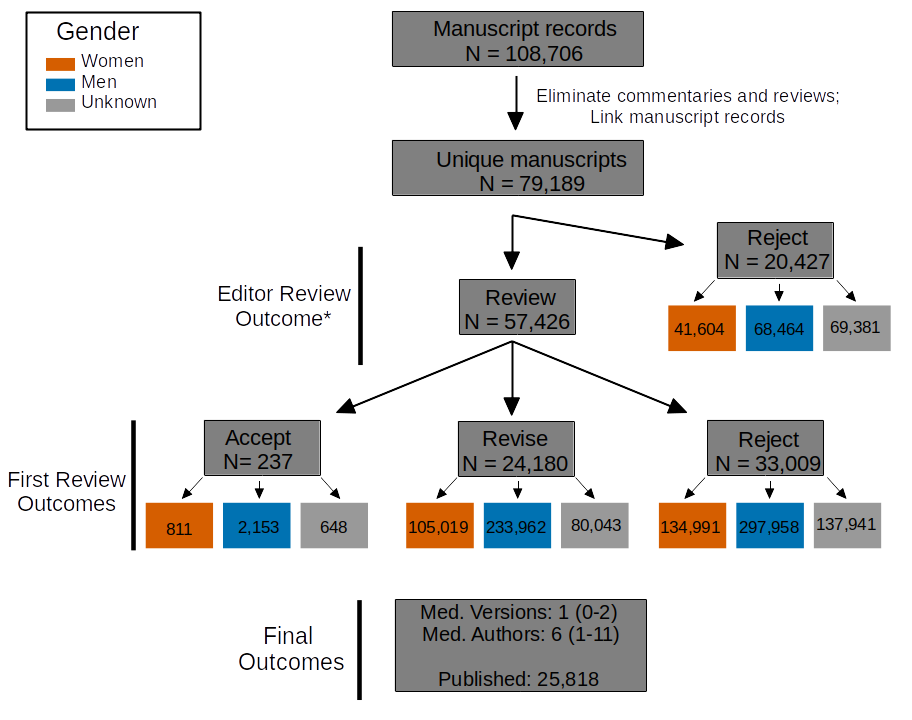
\includegraphics{population_diagram.png} \textbf{Figure 1. Overview of
manuscript outcomes.} 108,706 manuscript records were obtained for the
period between January 2012 and August 2018. After eliminating
non-primary research manuscripts and linking records for resubmitted
manuscripts, we processed 79,189 unique manuscripts. The median number
of versions was 1 (IQR=0-2) with a median of 6 (IQR=1-11) authors per
manuscript. As of August 2018, 34,196 of these were published at ASM
journals. Revisions were requested for 24,016 manuscripts and 53,436
manuscripts were rejected at their first submission. The number of
individuals (e.g., author, editor, reviewer) involved in each category
of manuscript decision are indicated in the colored boxes: women
(orange), men (blue), and unknown (gray). *A small number were given
revise (242) or acceptance (1094) decisions without review.

\newpage

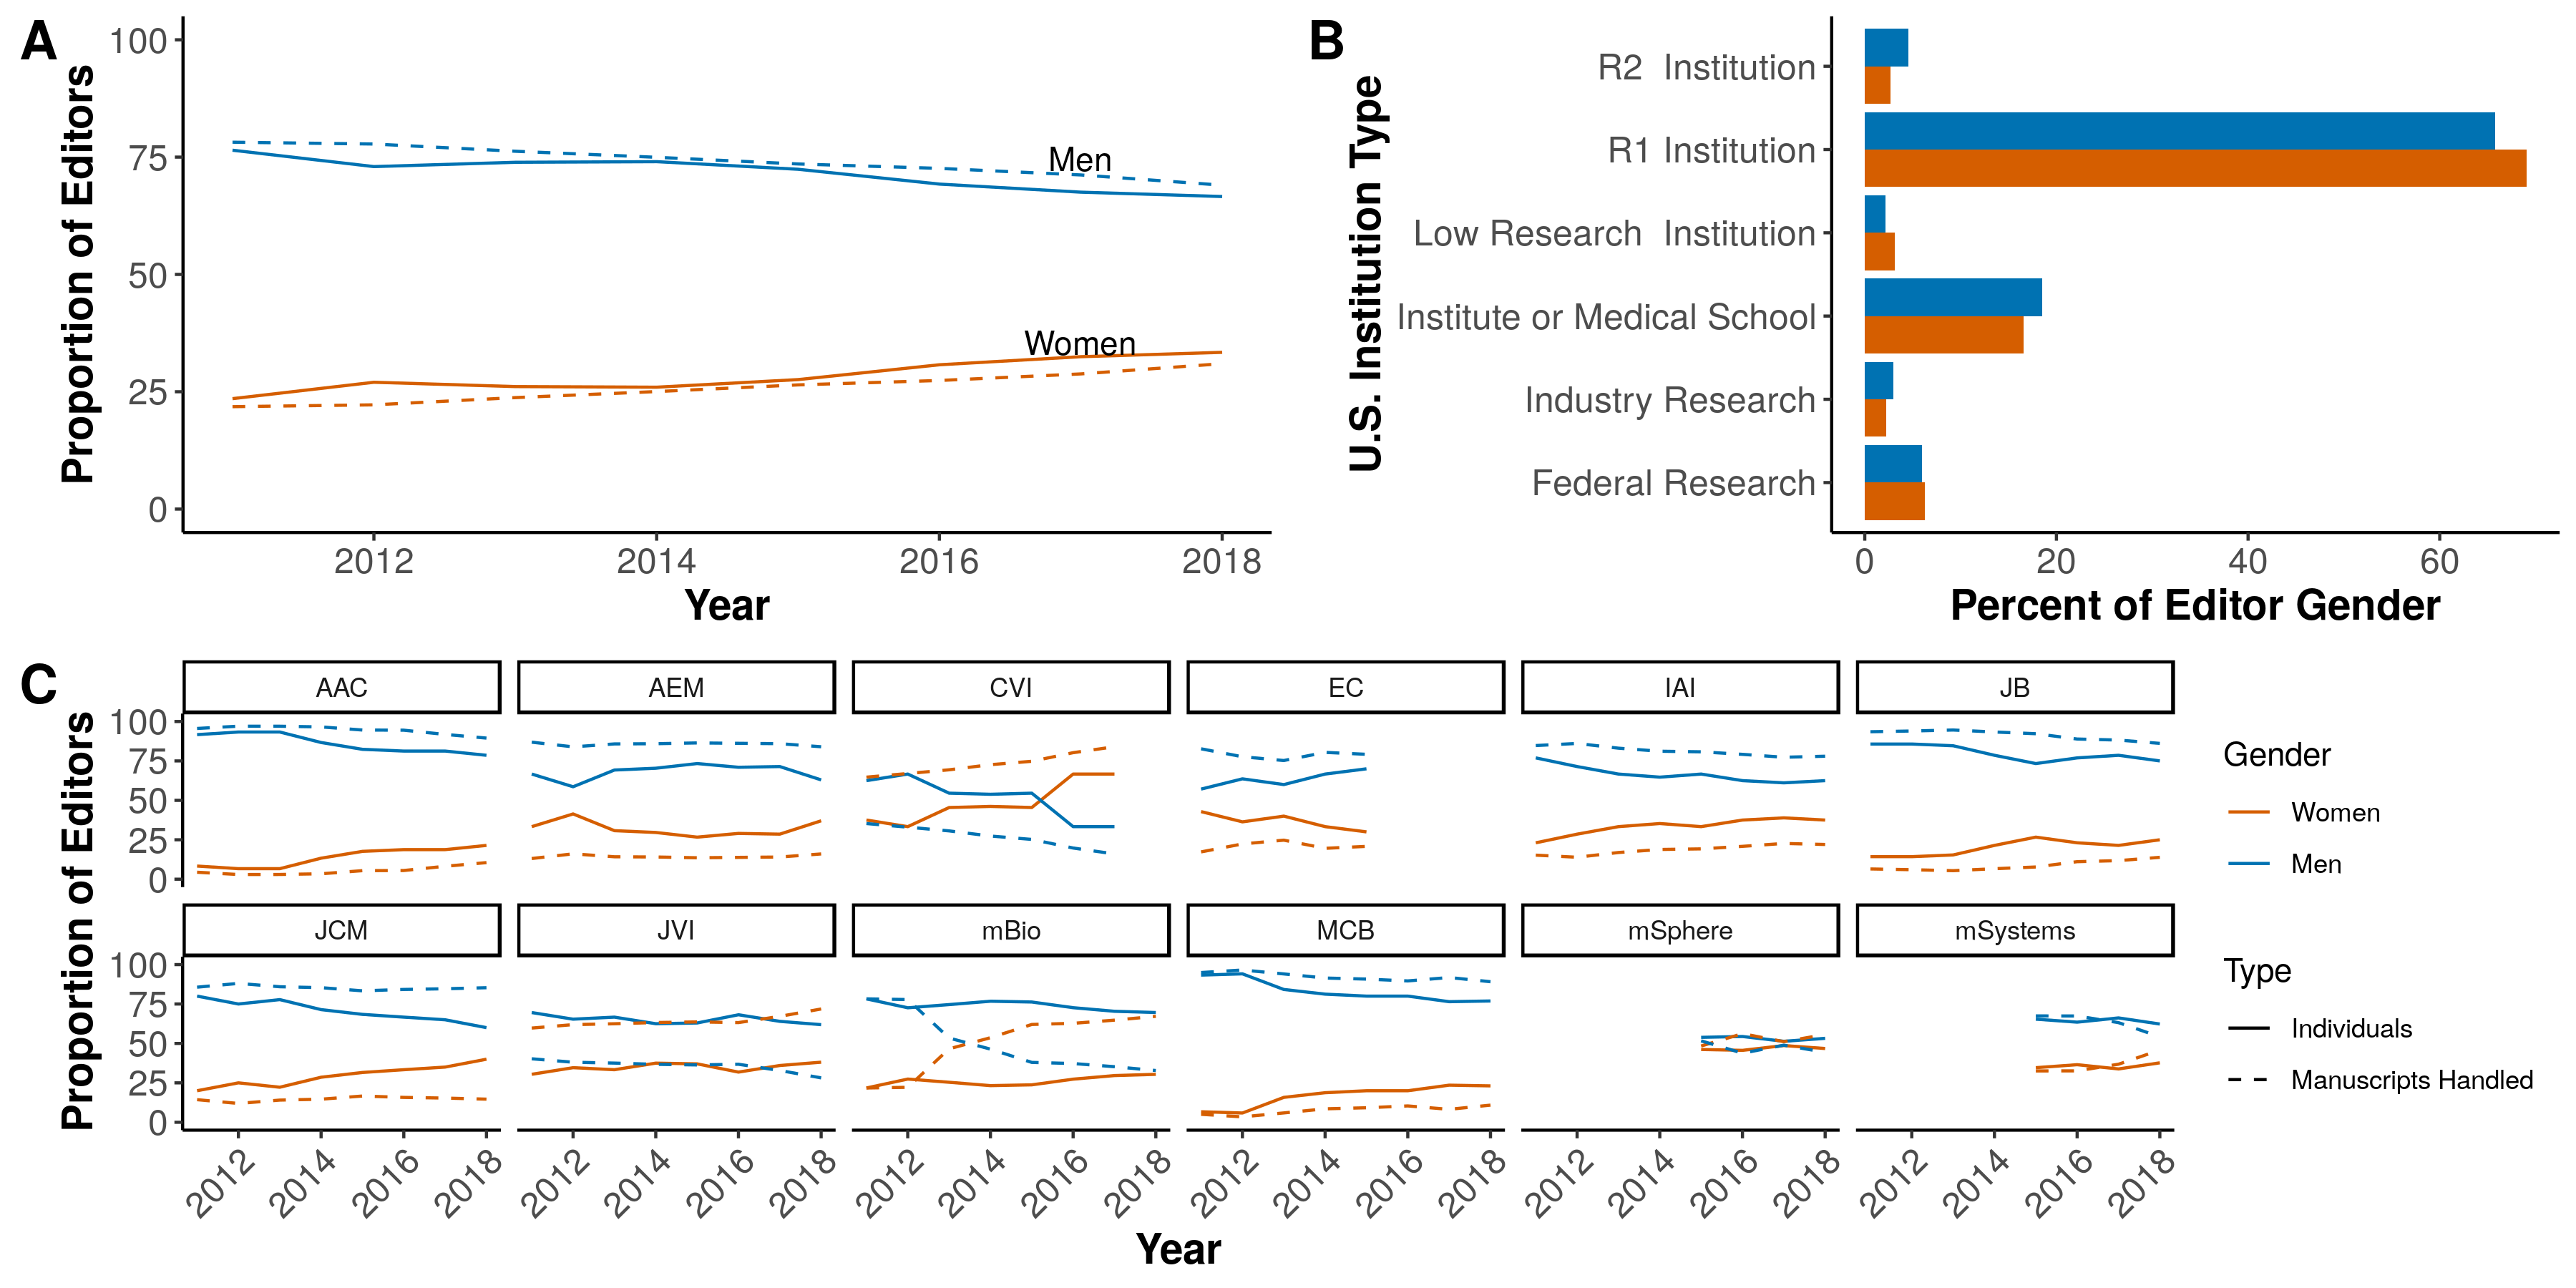
\includegraphics{Figure_1.png} \textbf{Figure 2. Gendered representation
among gatekeepers.} Proportion of editors from (A) institution types and
(B) over time. Editors and senior editors are pooled together.
Proportion of reviewers from (C) institution types and (D) over time.
(A,C) Each gender equals 100\% when all institutions are summed.(B,D)
Each individual was counted once per calendar year, proportions of each
gender add to 100\% per year.

\newpage

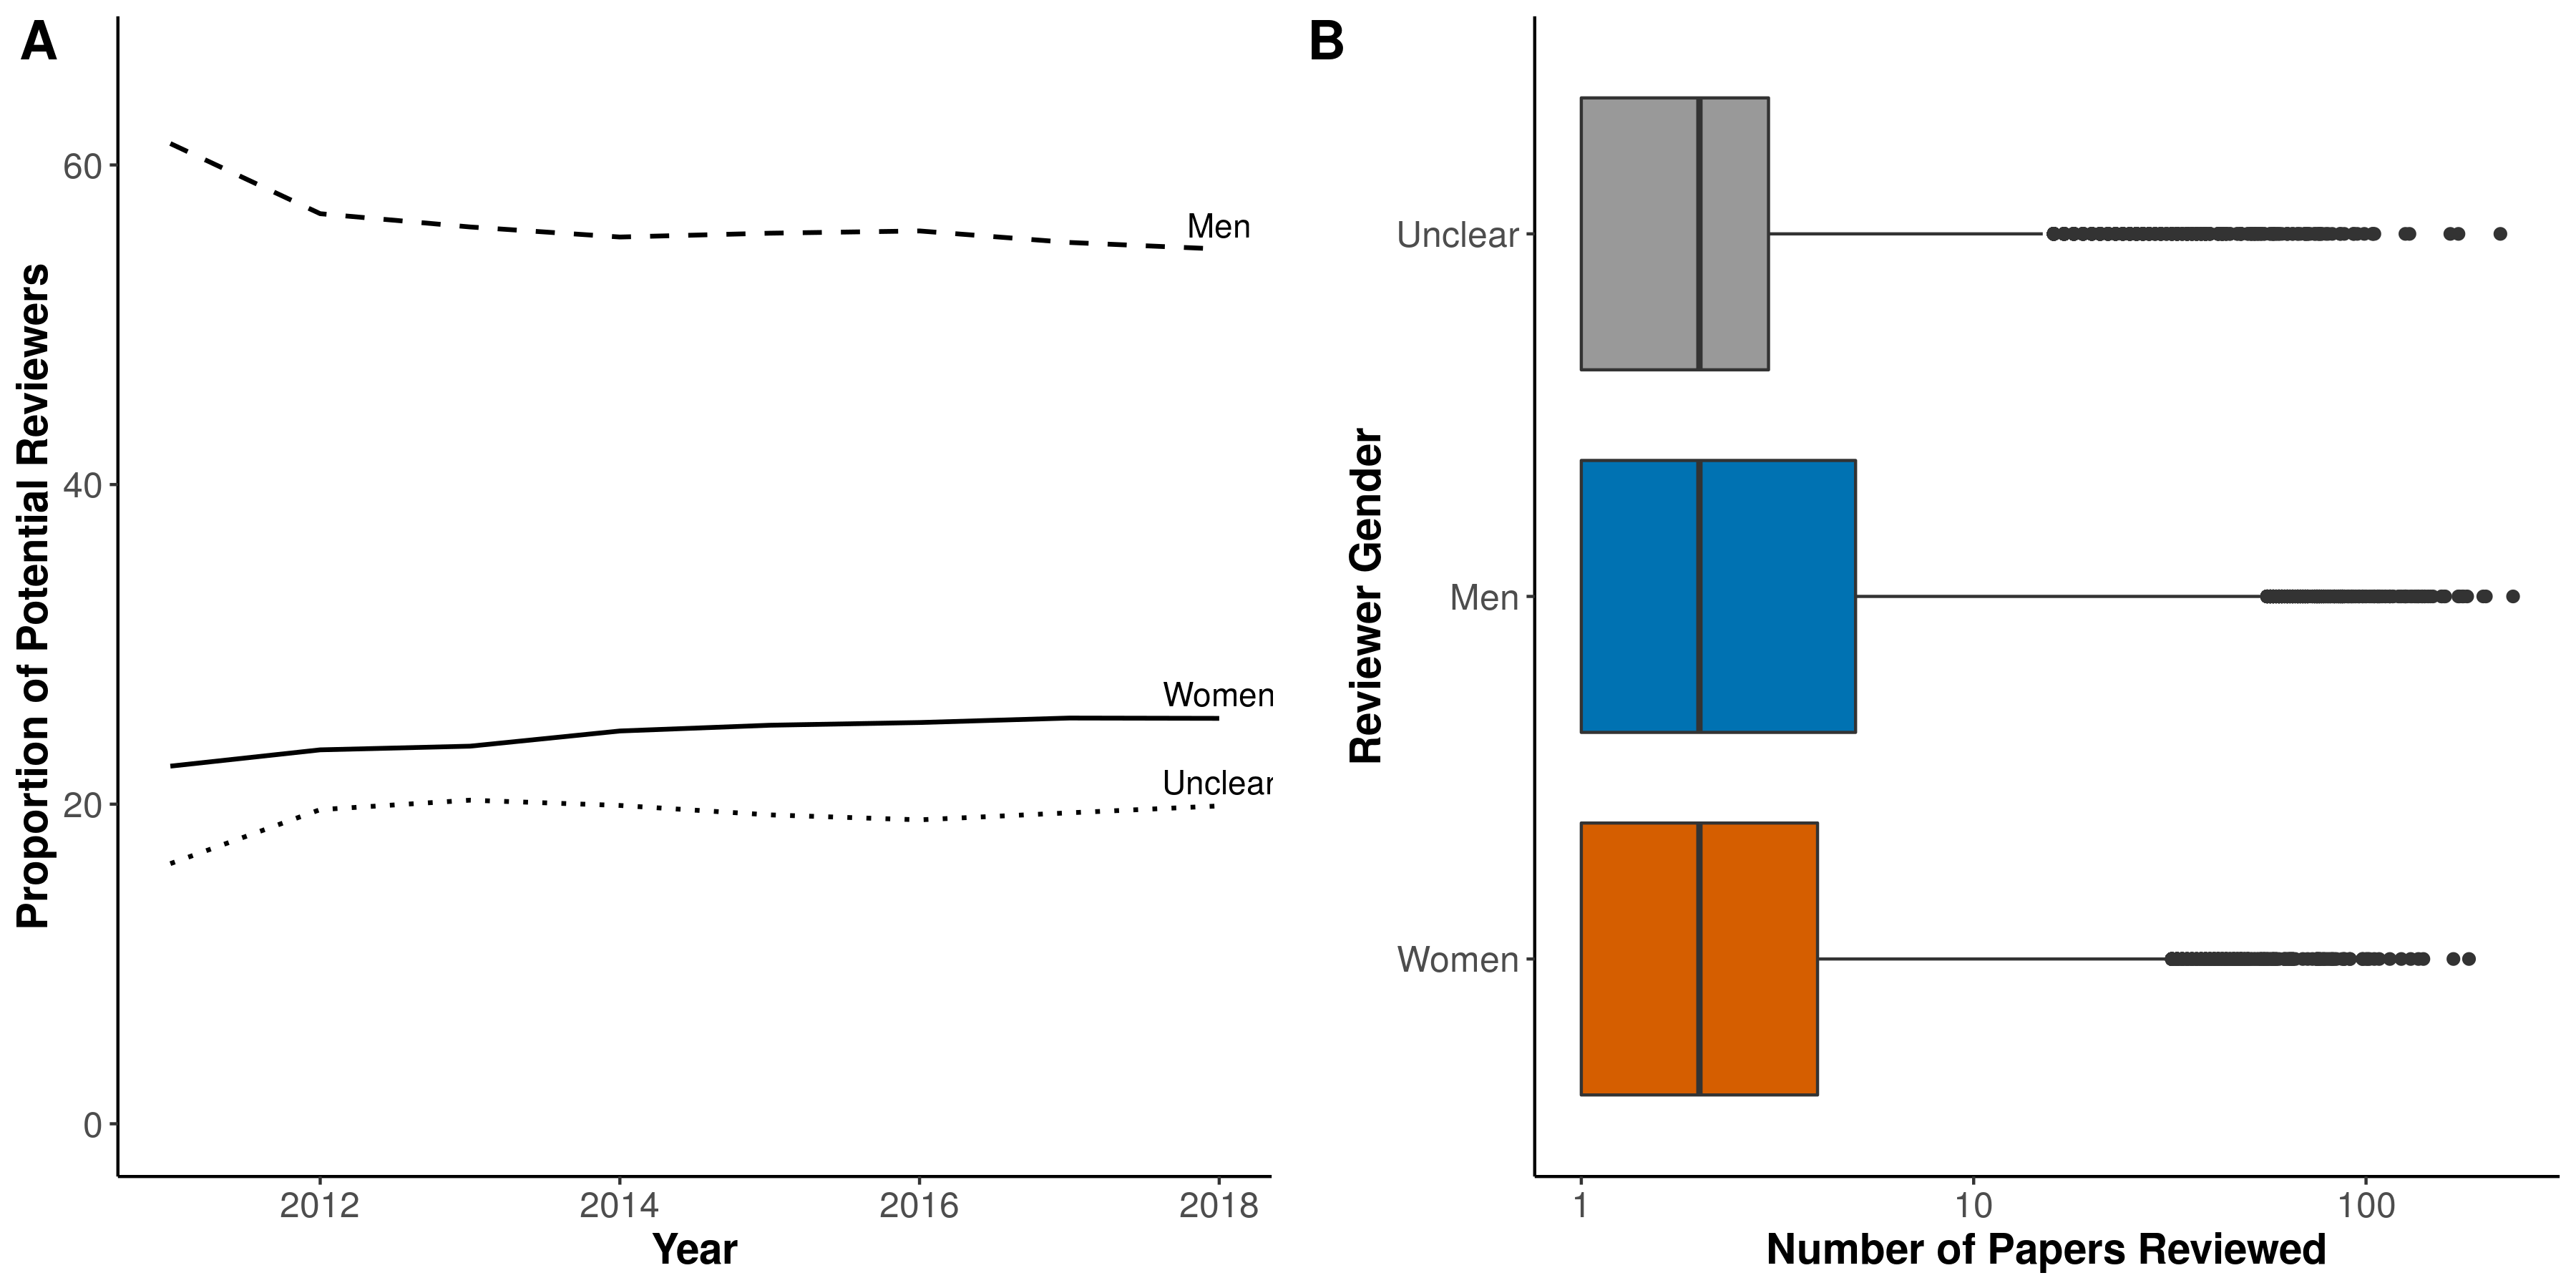
\includegraphics{Figure_2.png} \textbf{Figure 3. Gatekeeper workload and
response to requests to review.} (A) Proportion of manuscript workloads
by men and women editors, editorial rejections excluded. (B) Box plot
comparison of all manuscripts, by reviewer gender. (C) The percent of
reviewers by gender that accepted the opportunity to review, split
according to the editor's gender.

\newpage

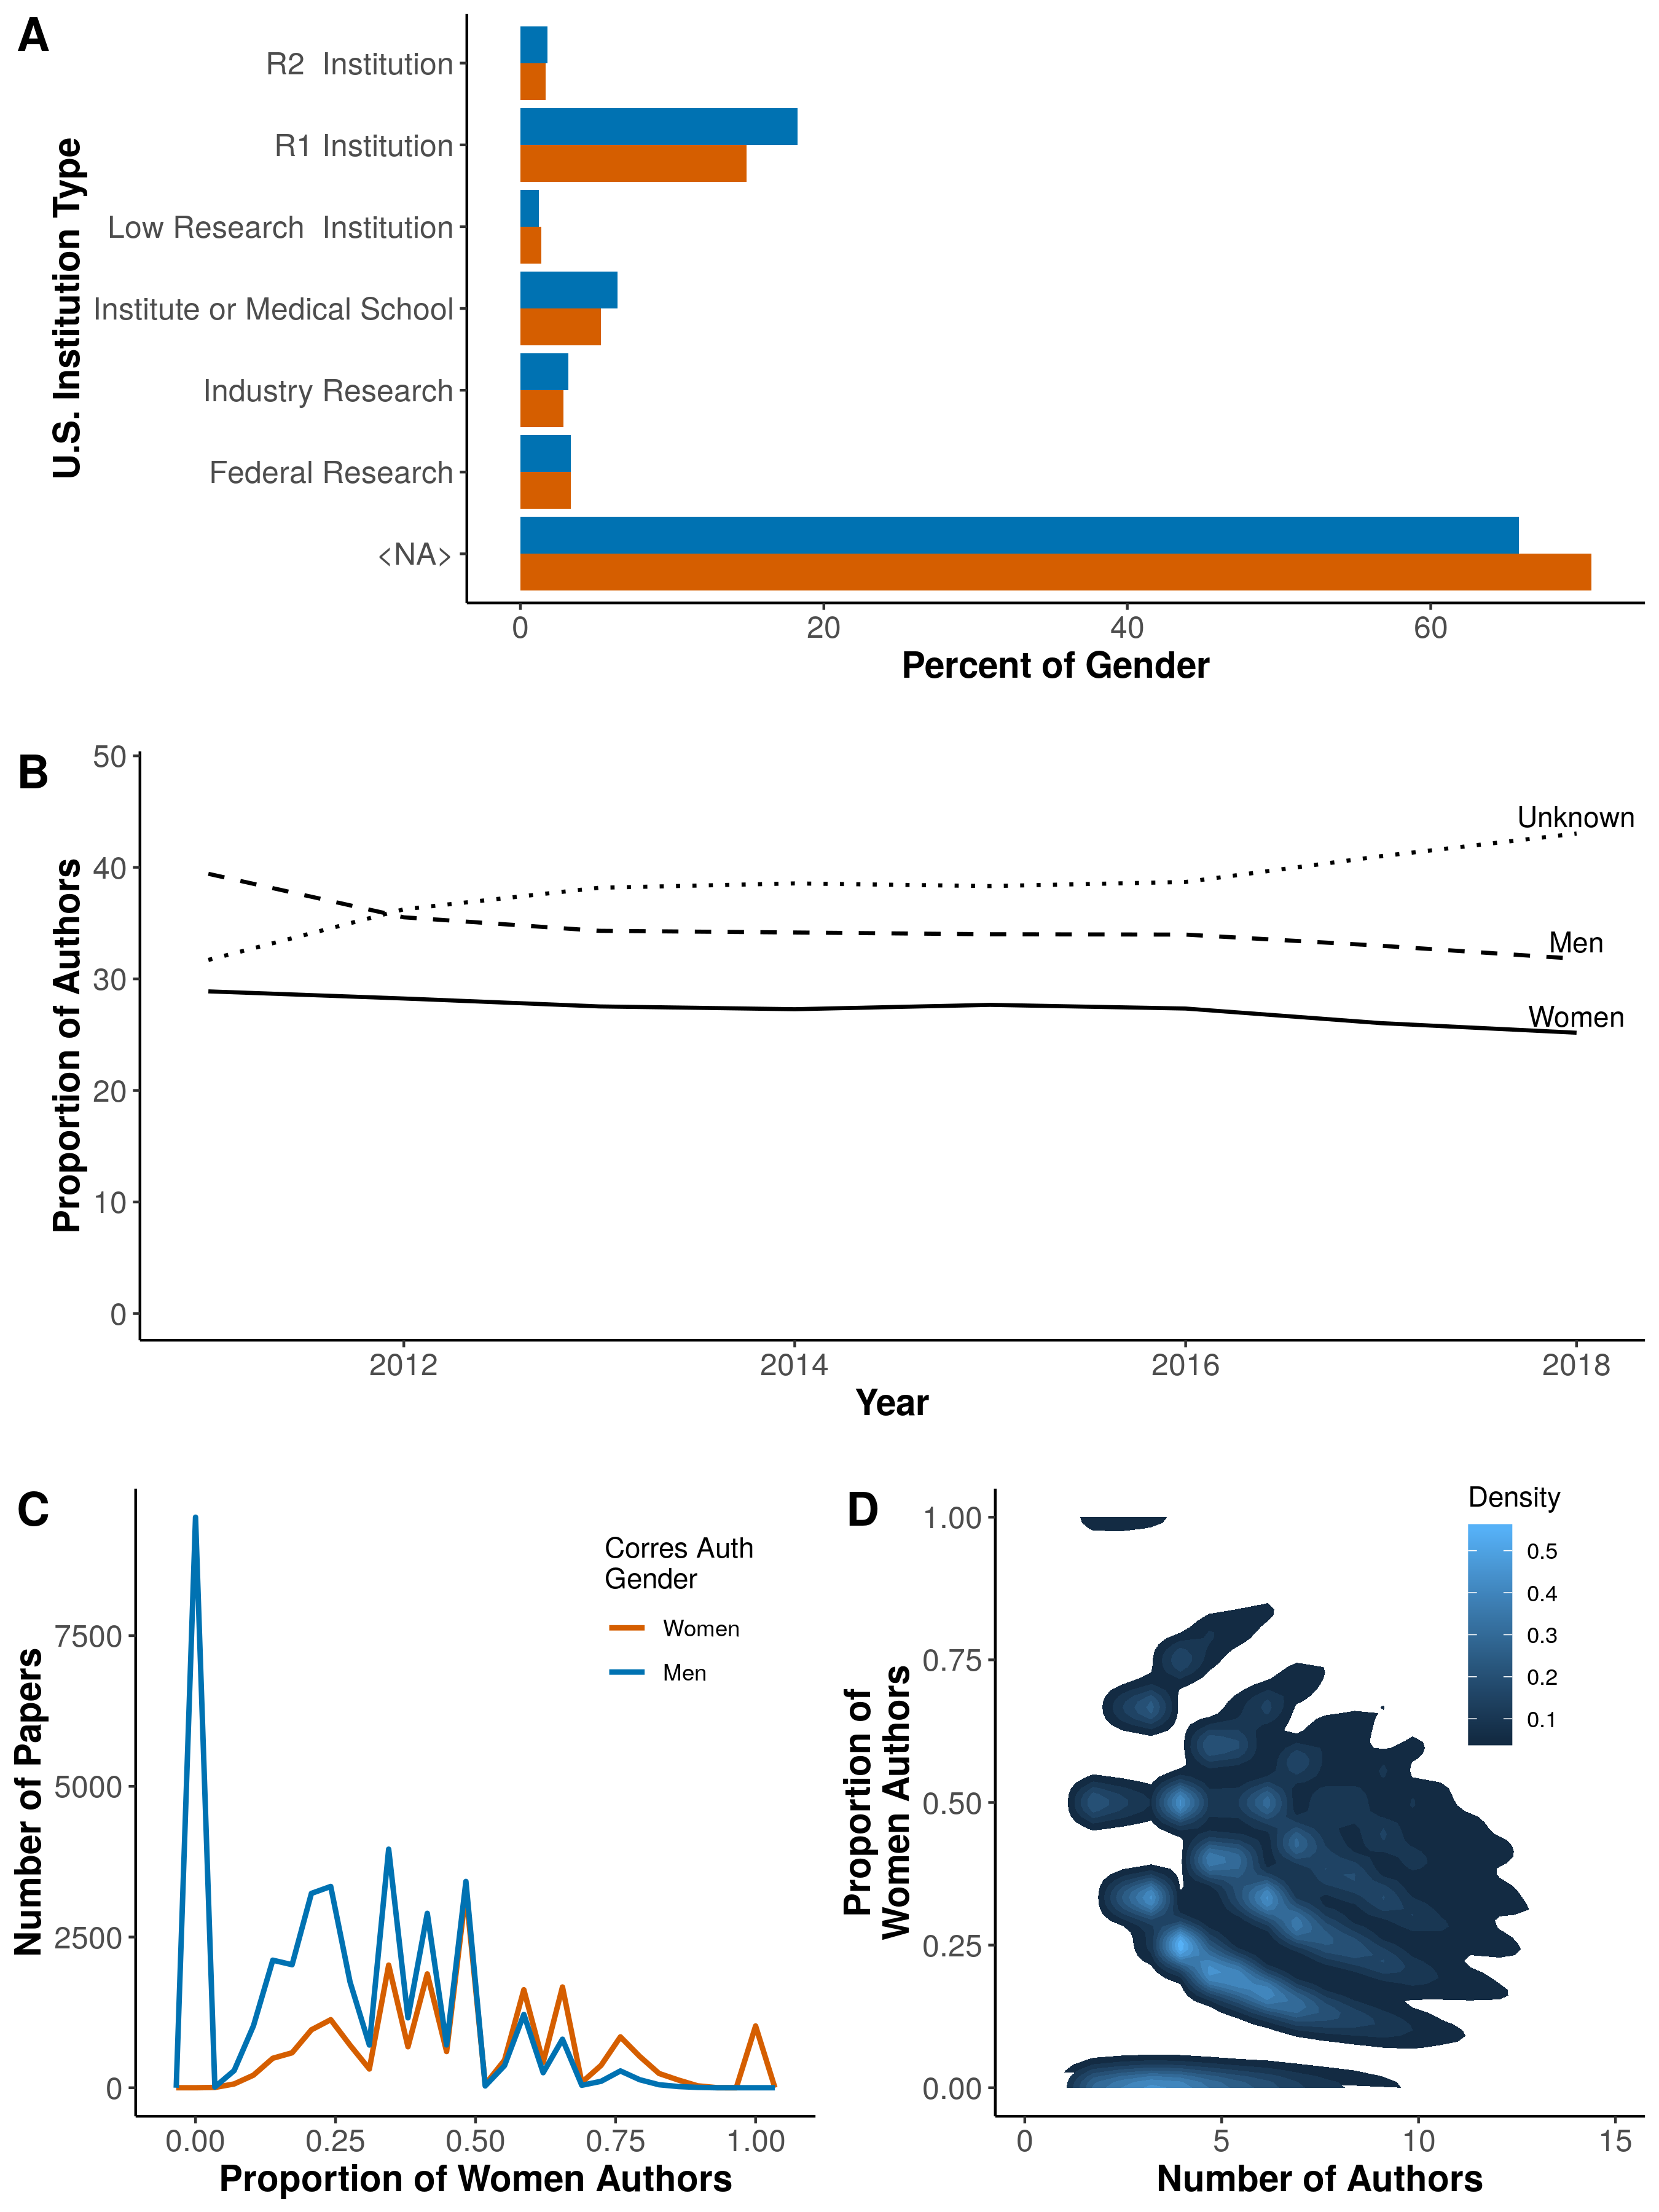
\includegraphics{Figure_3.png} \textbf{Figure 4. Author representation
by gender.} The proportion of (A) men and women senior authors from each
institution type, (B) men, women, and unknown authors from 2012 - 2018.
Each individual was counted once per calendar year. The proportion of
(C) first authors and (D) corresponding authors from 2012 - 2018 on
submitted manuscripts (dashed line) and published papers (solid line).

\newpage

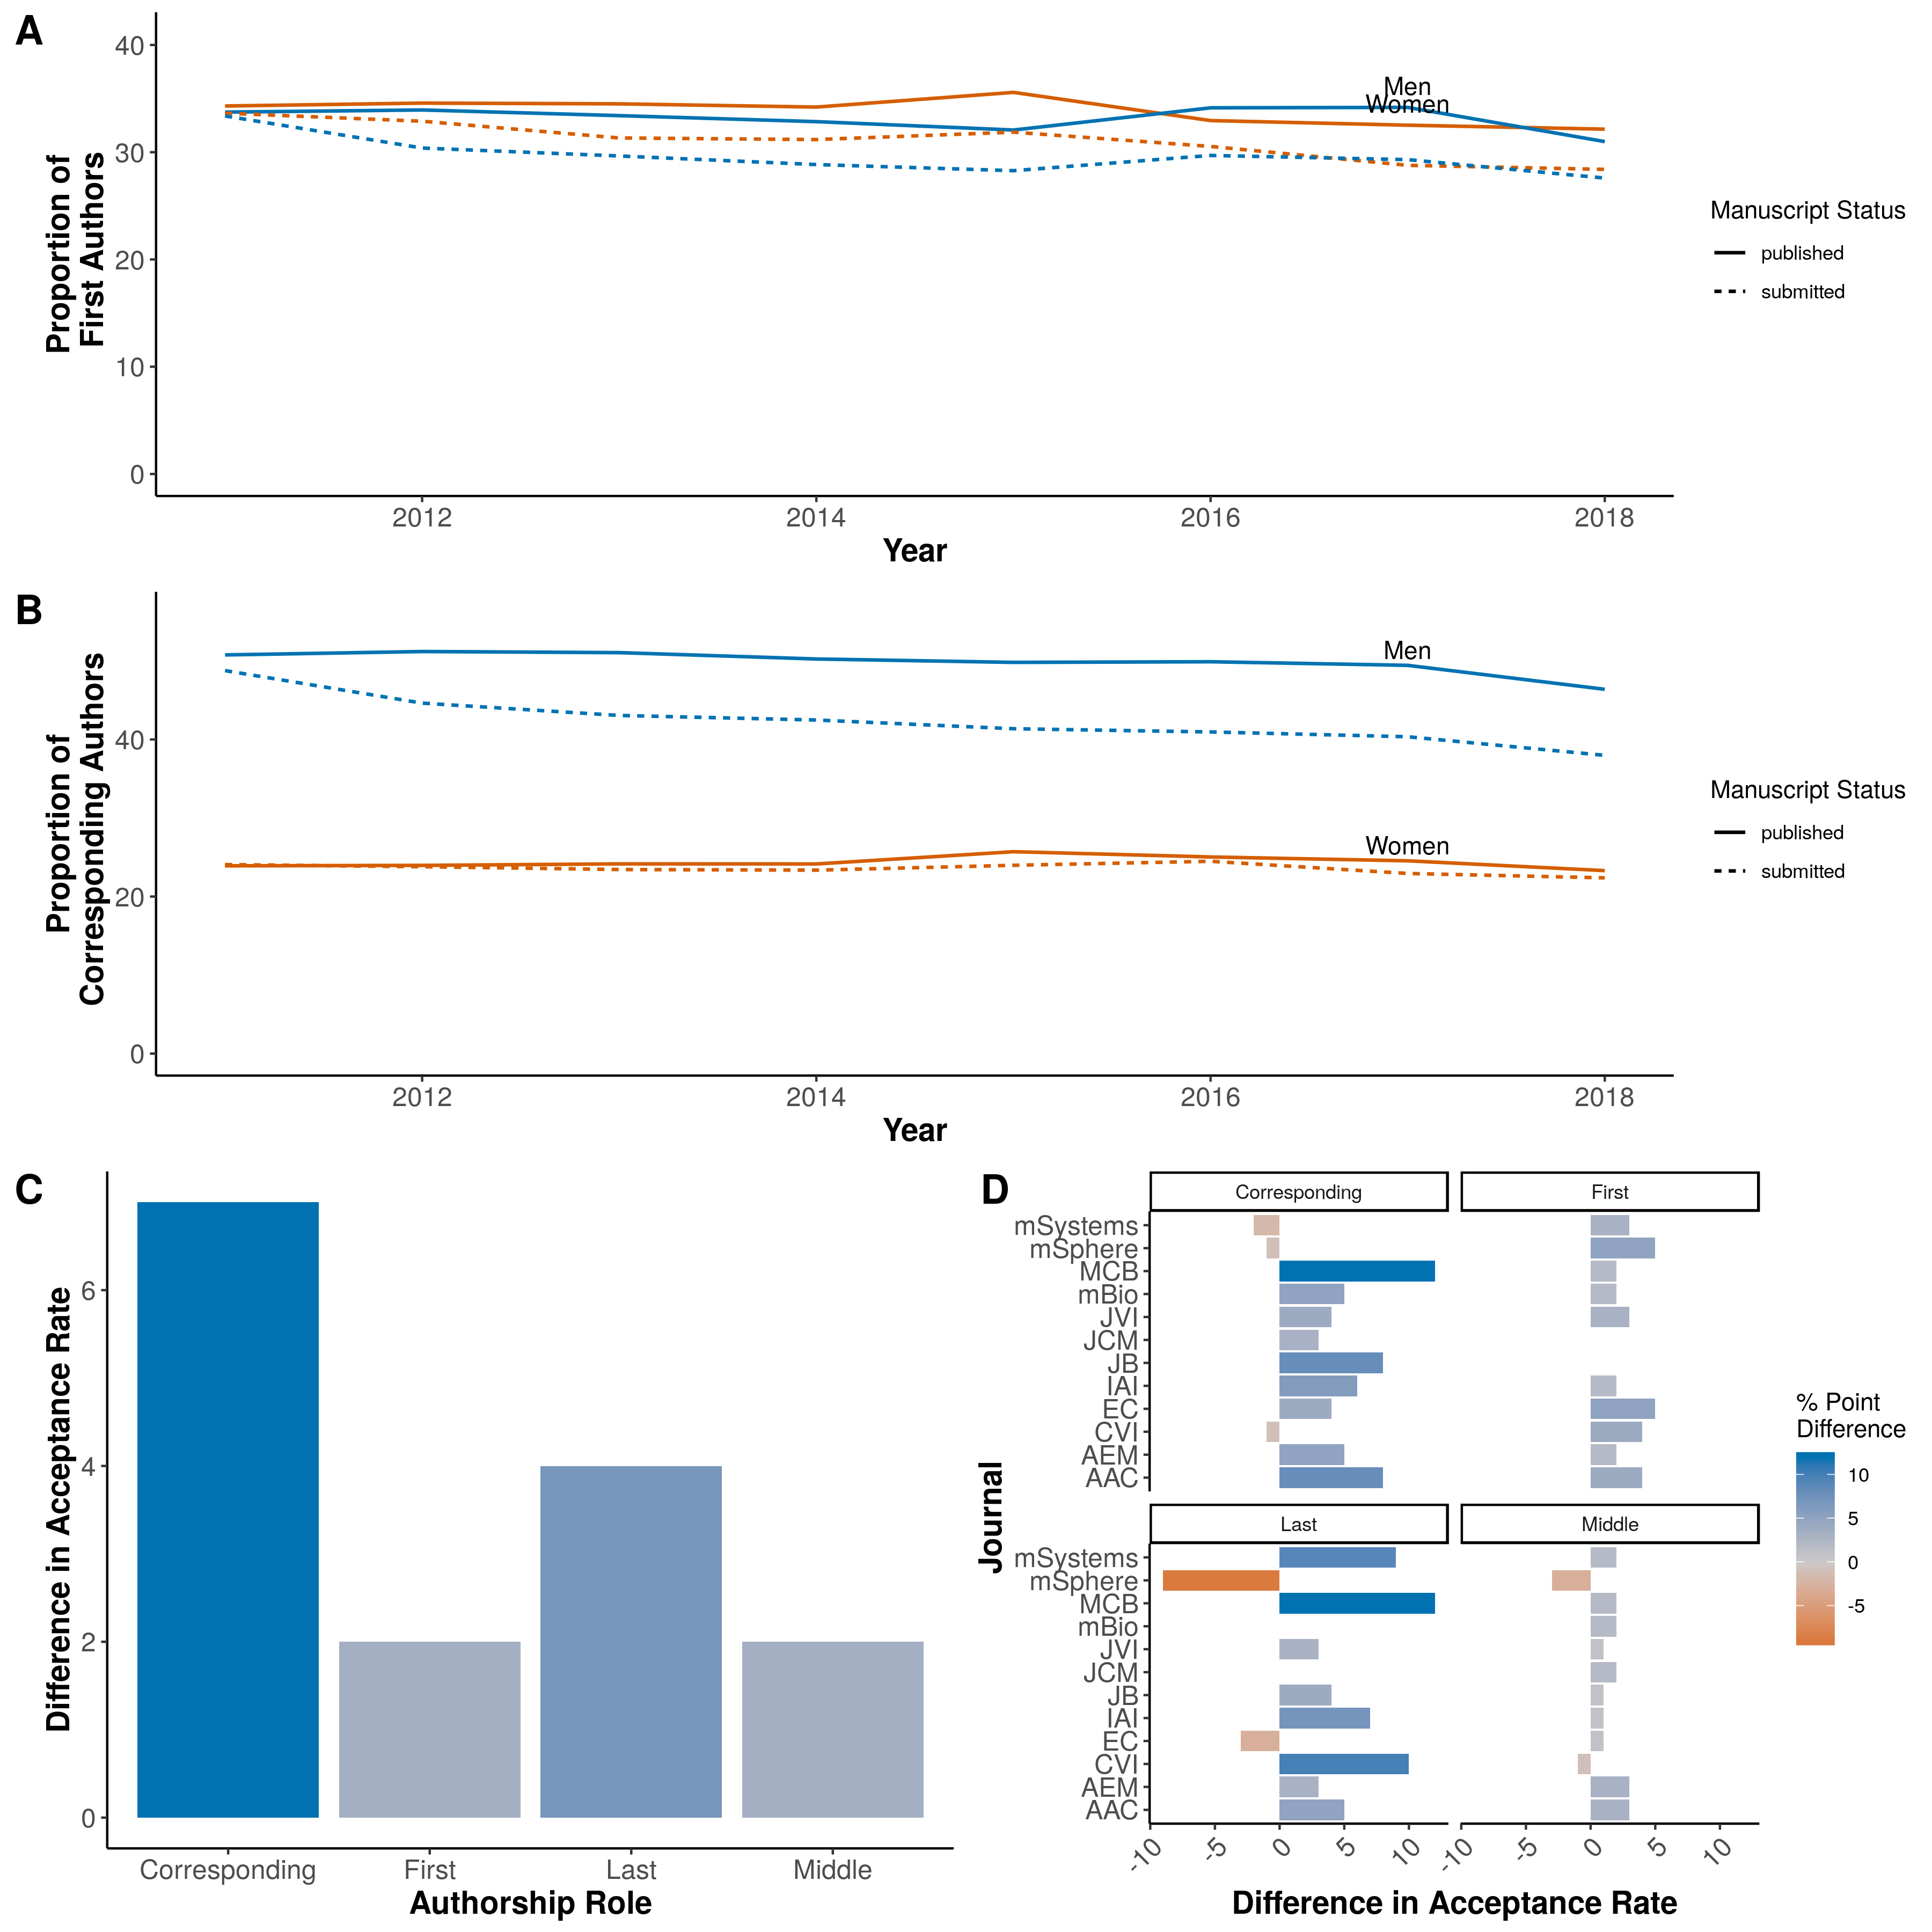
\includegraphics{Figure_4.png} \textbf{Figure 5. Difference in
manuscript outcomes by author gender.} (A) The percent of manuscripts
rejected by author gender and type (e.g., corresponding, first, last,
middle) at any stage across all journals where 0 indicates equal rates
of rejection. (B) The difference in percent editorial rejection rates
for corresponding authors at each journal. (C) The difference in
percentage points between each decision type for corresponding authors
following the first peer review. Vertical lines indicate the difference
value for all journals combined. Absence of a bar indicates no
difference, or parity.

\newpage

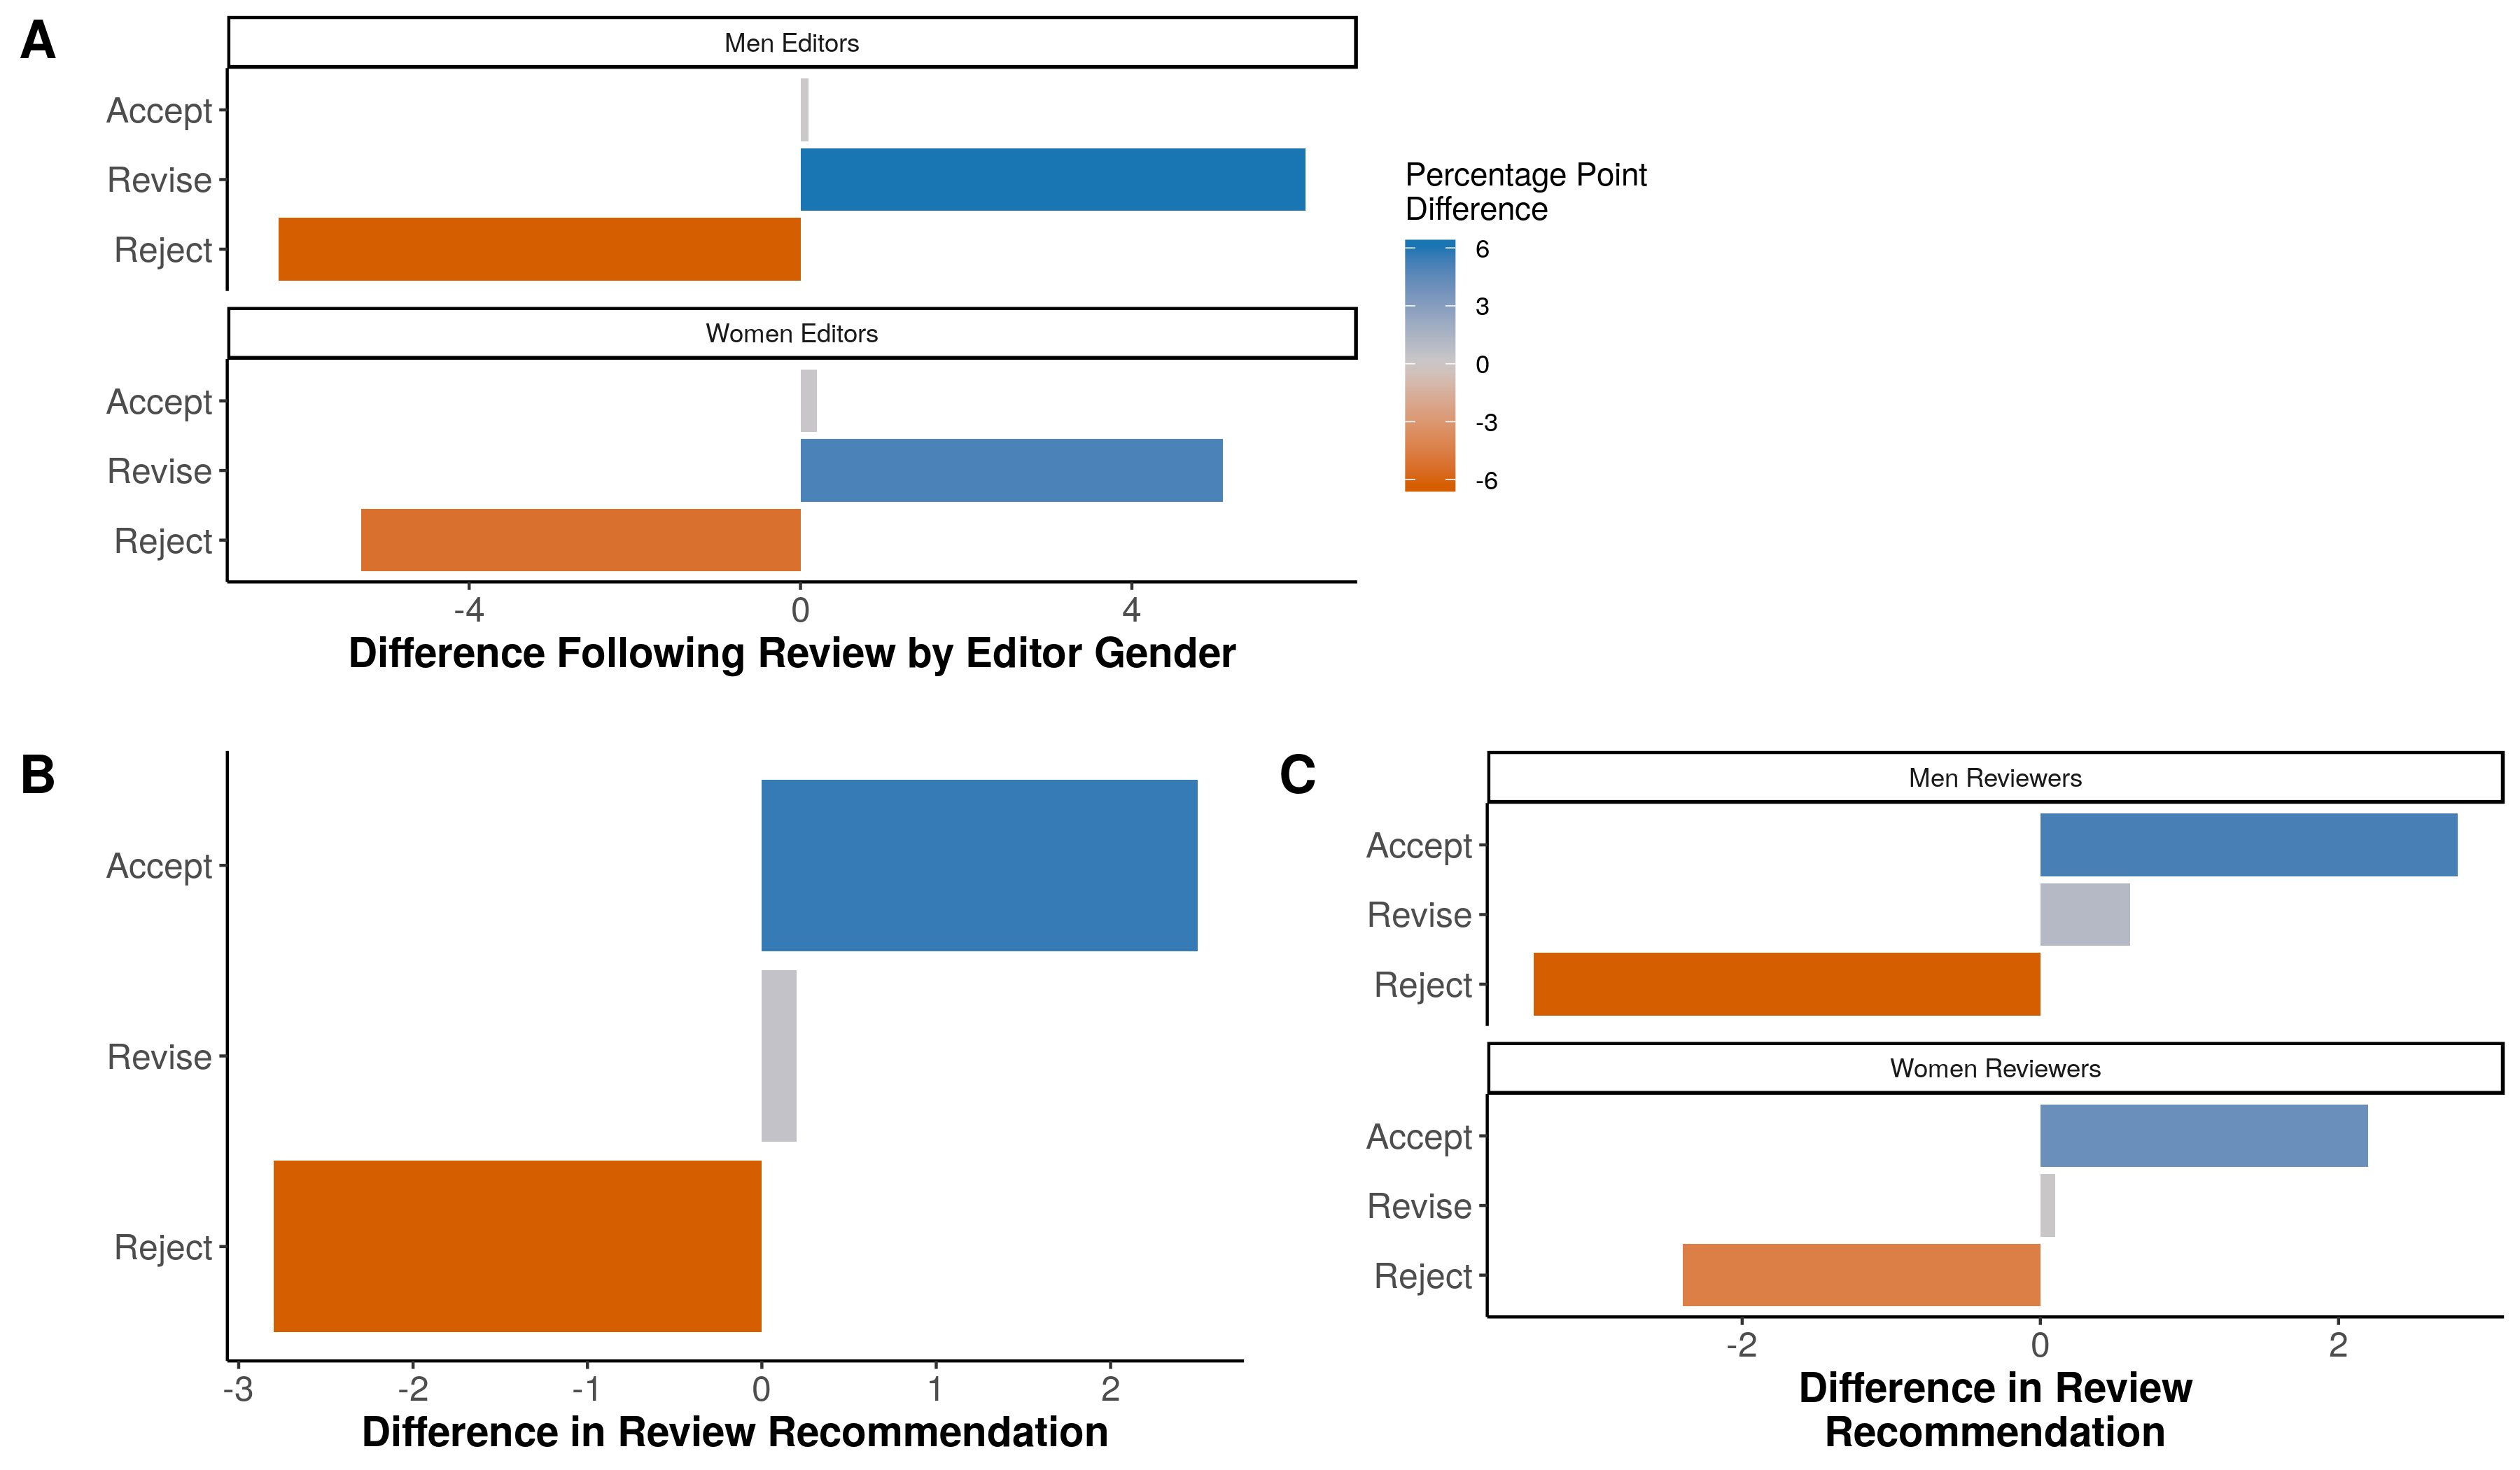
\includegraphics{Figure_5.png} \textbf{Figure 6. Difference in decisions
or recomendations according to the gatekeeper gender.} (A) Effect of
editor gender on the difference in decisions following review. (B)
Difference in percentage points for review recommendations and (C) how
that is affected by reviewer gender. (A-C) All journals combined.

\newpage

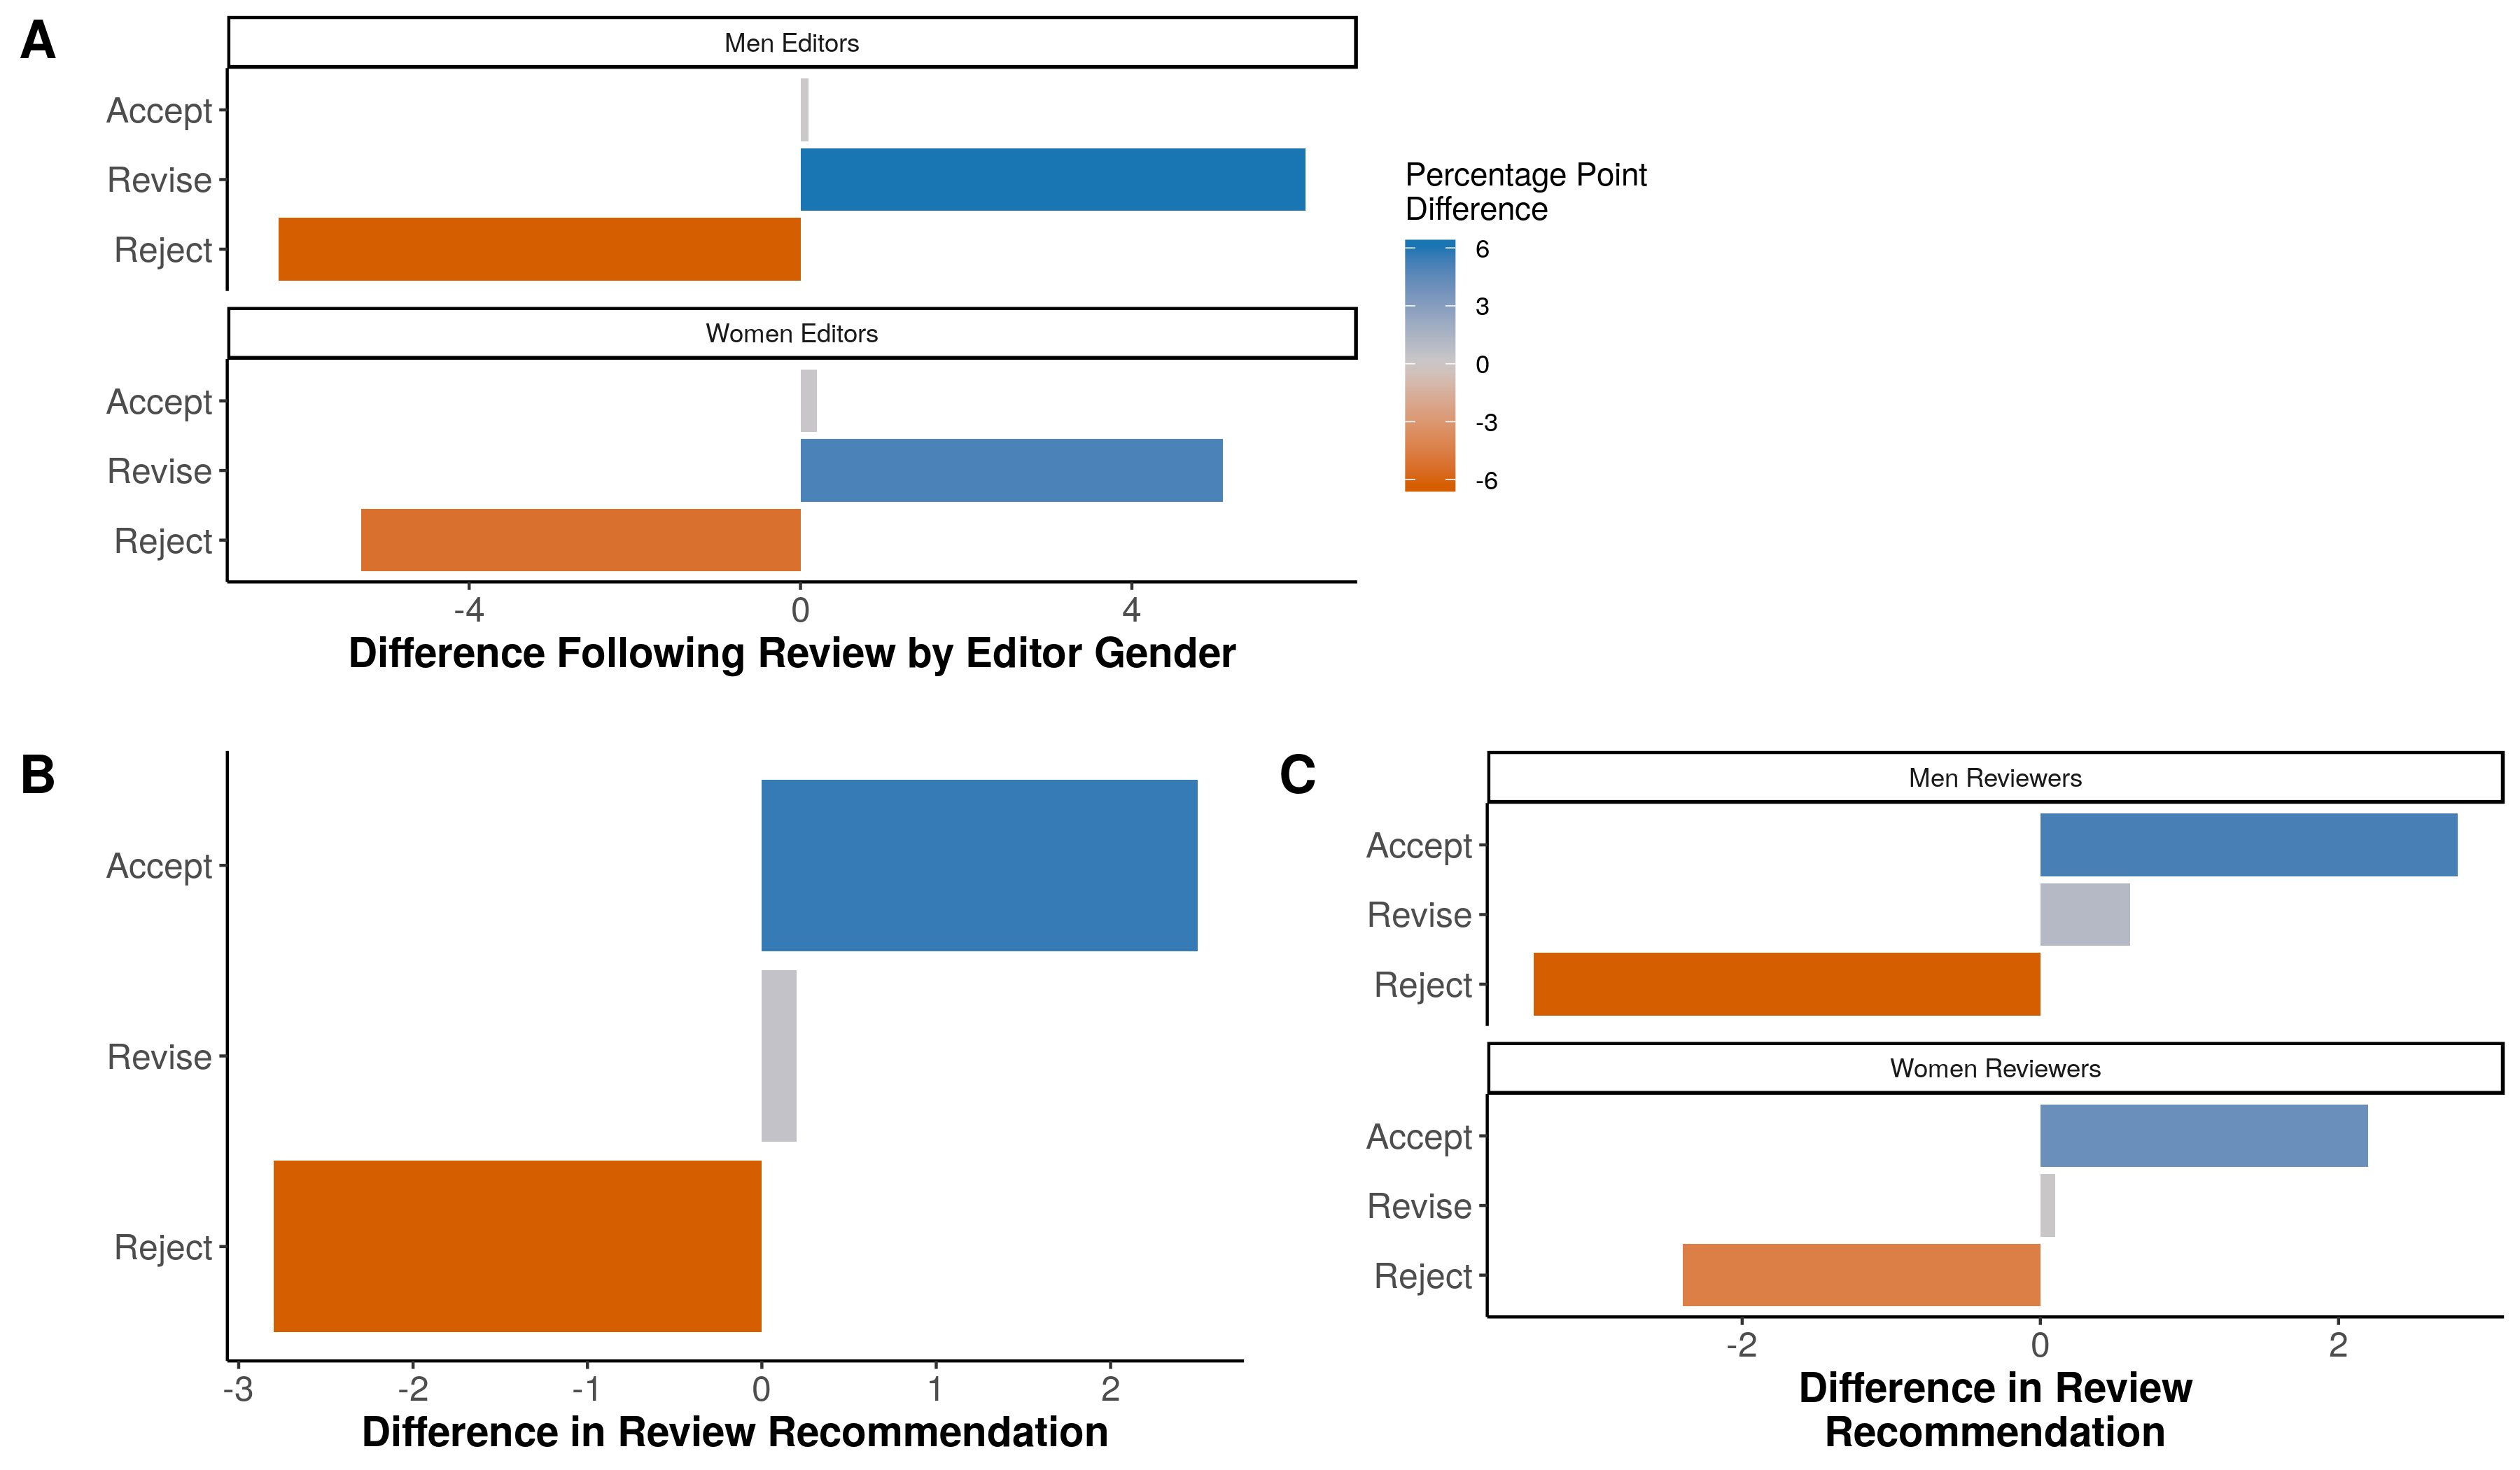
\includegraphics{Figure_6.png} \textbf{Figure 7. Impact of origin and
U.S. institution type on manuscript decisions by gender.} Difference in
percentage points for (A) editorial rejections and (B) following first
review of manuscripts submitted by US-based corresponding authors.
Vertical line indicates value for all ASM journals combined. (C)
Difference in percentage points for acceptance and editorial rejections
according to institution types and (D) acceptance decisions by editor
gender and institution type.

\newpage

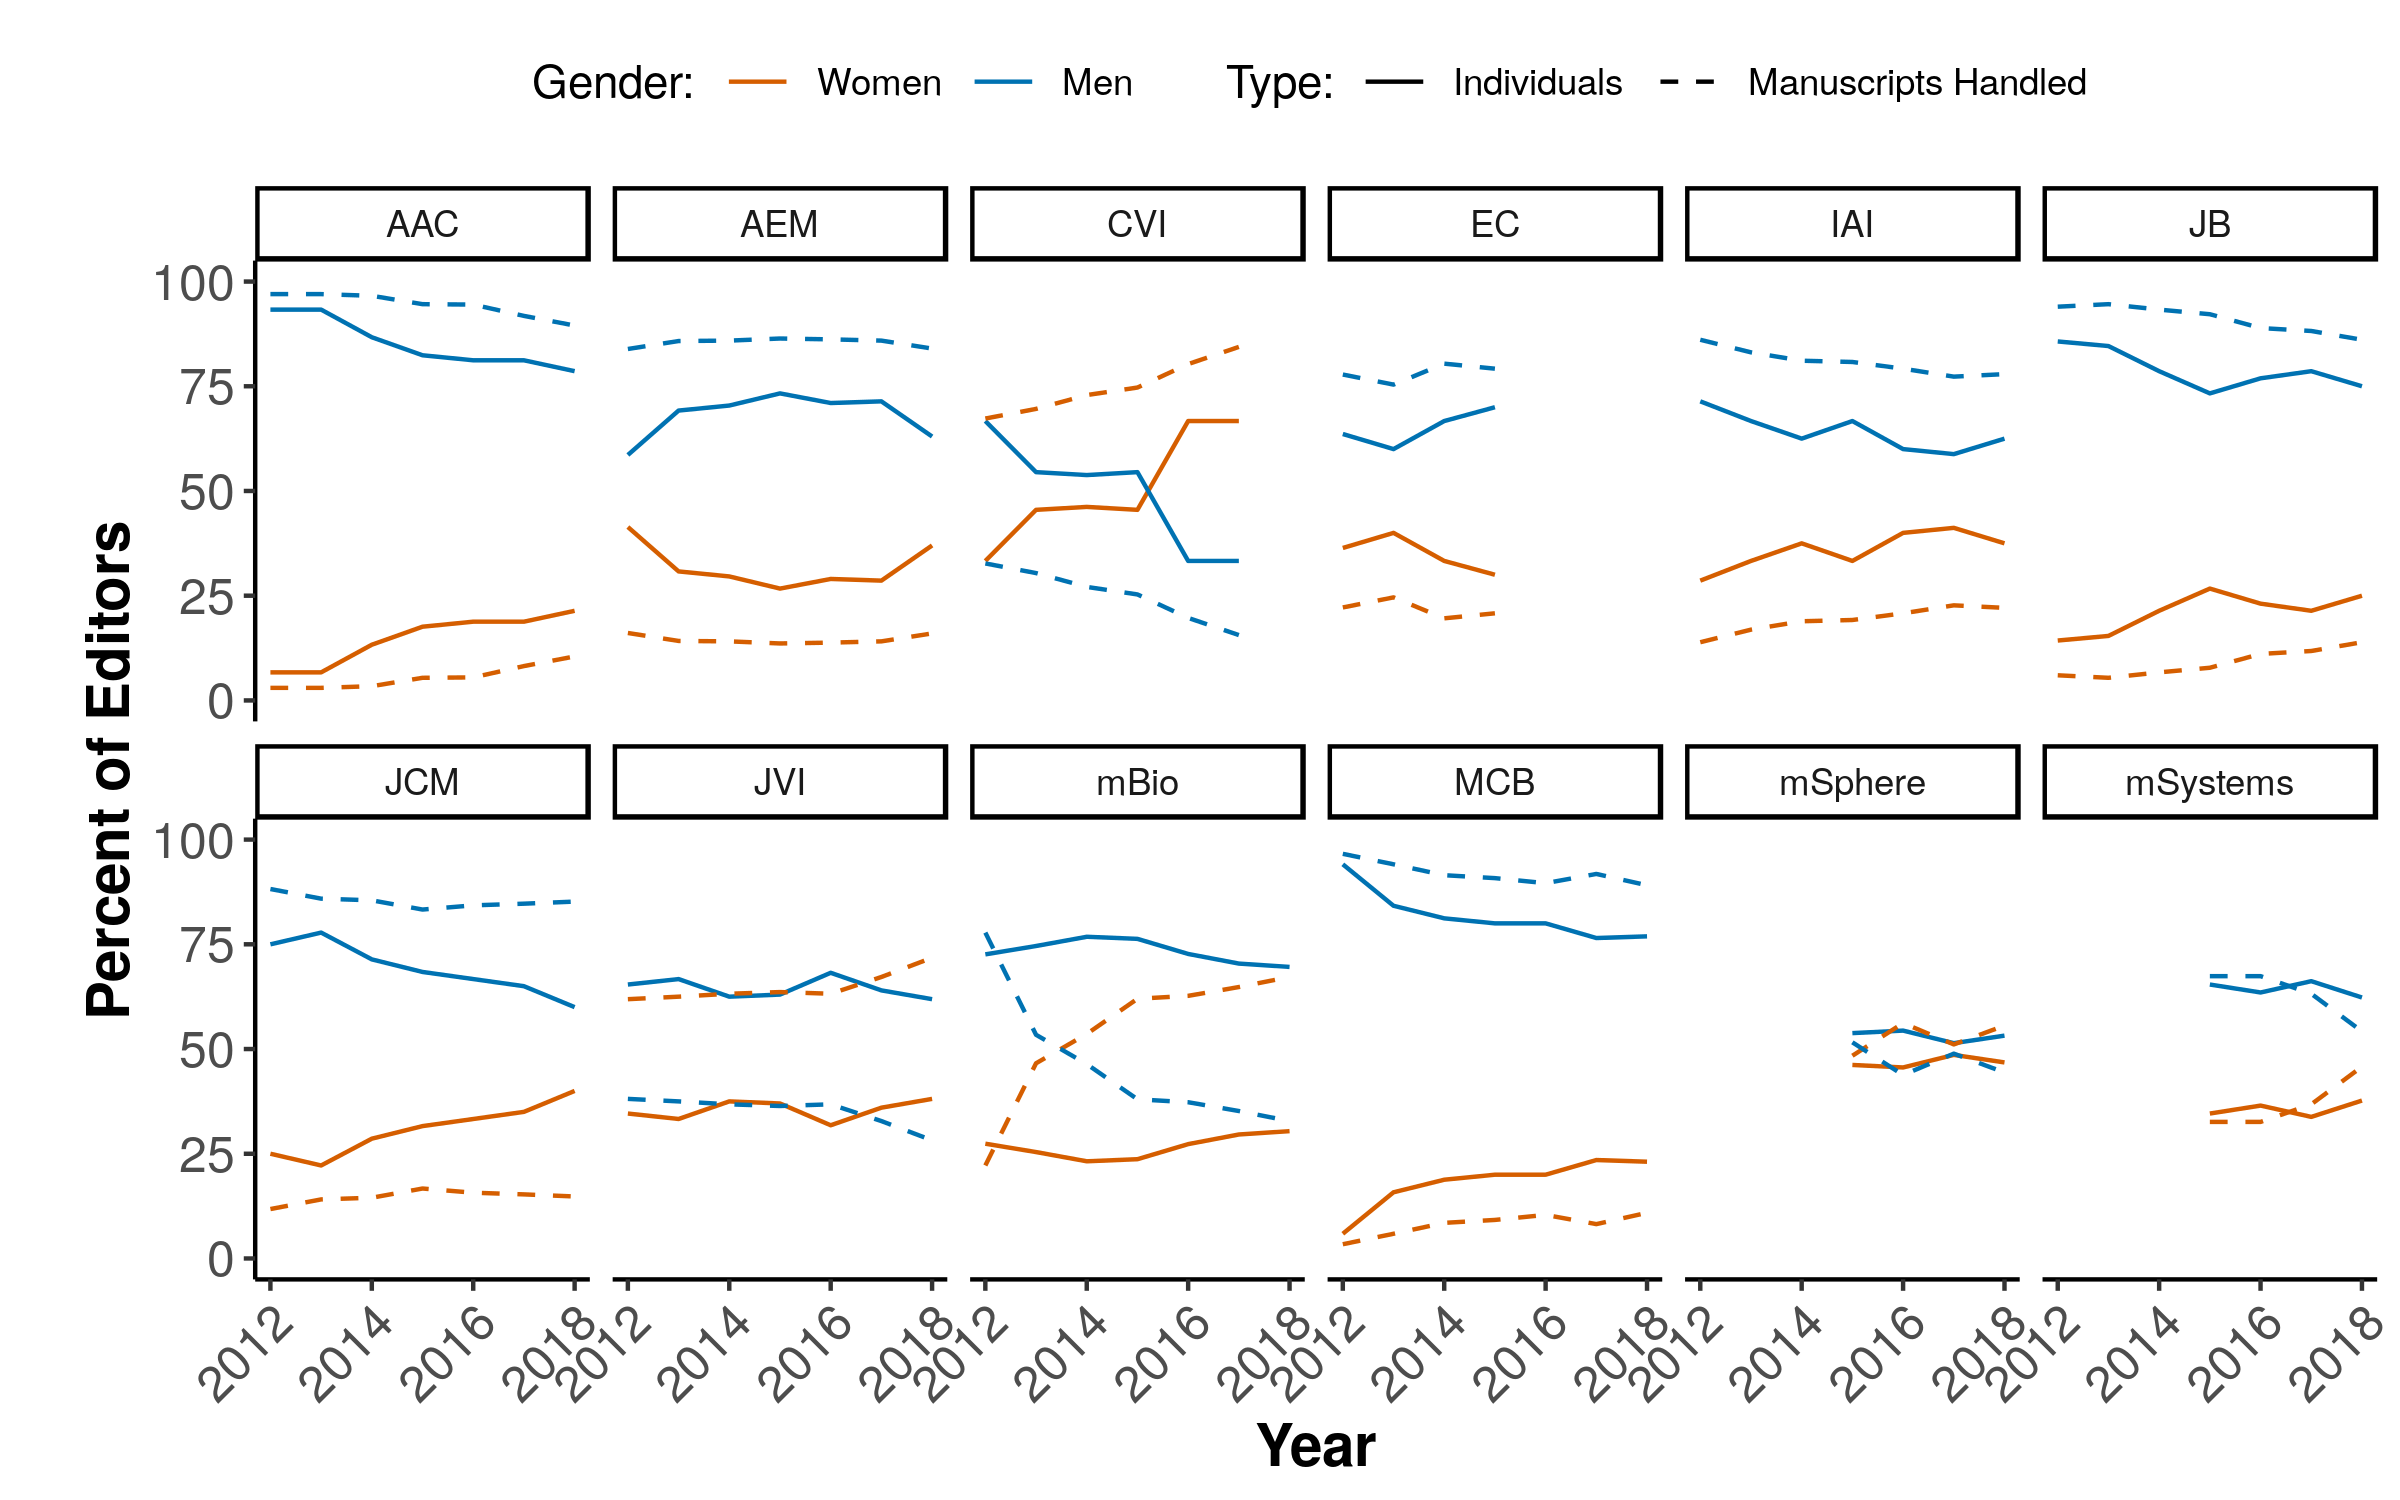
\includegraphics{Figure_S1.png} Figure S1. The proportion of editors
(solid line) and their workloads (dashed line) at each ASM journal from
2012 to 2018.

\newpage

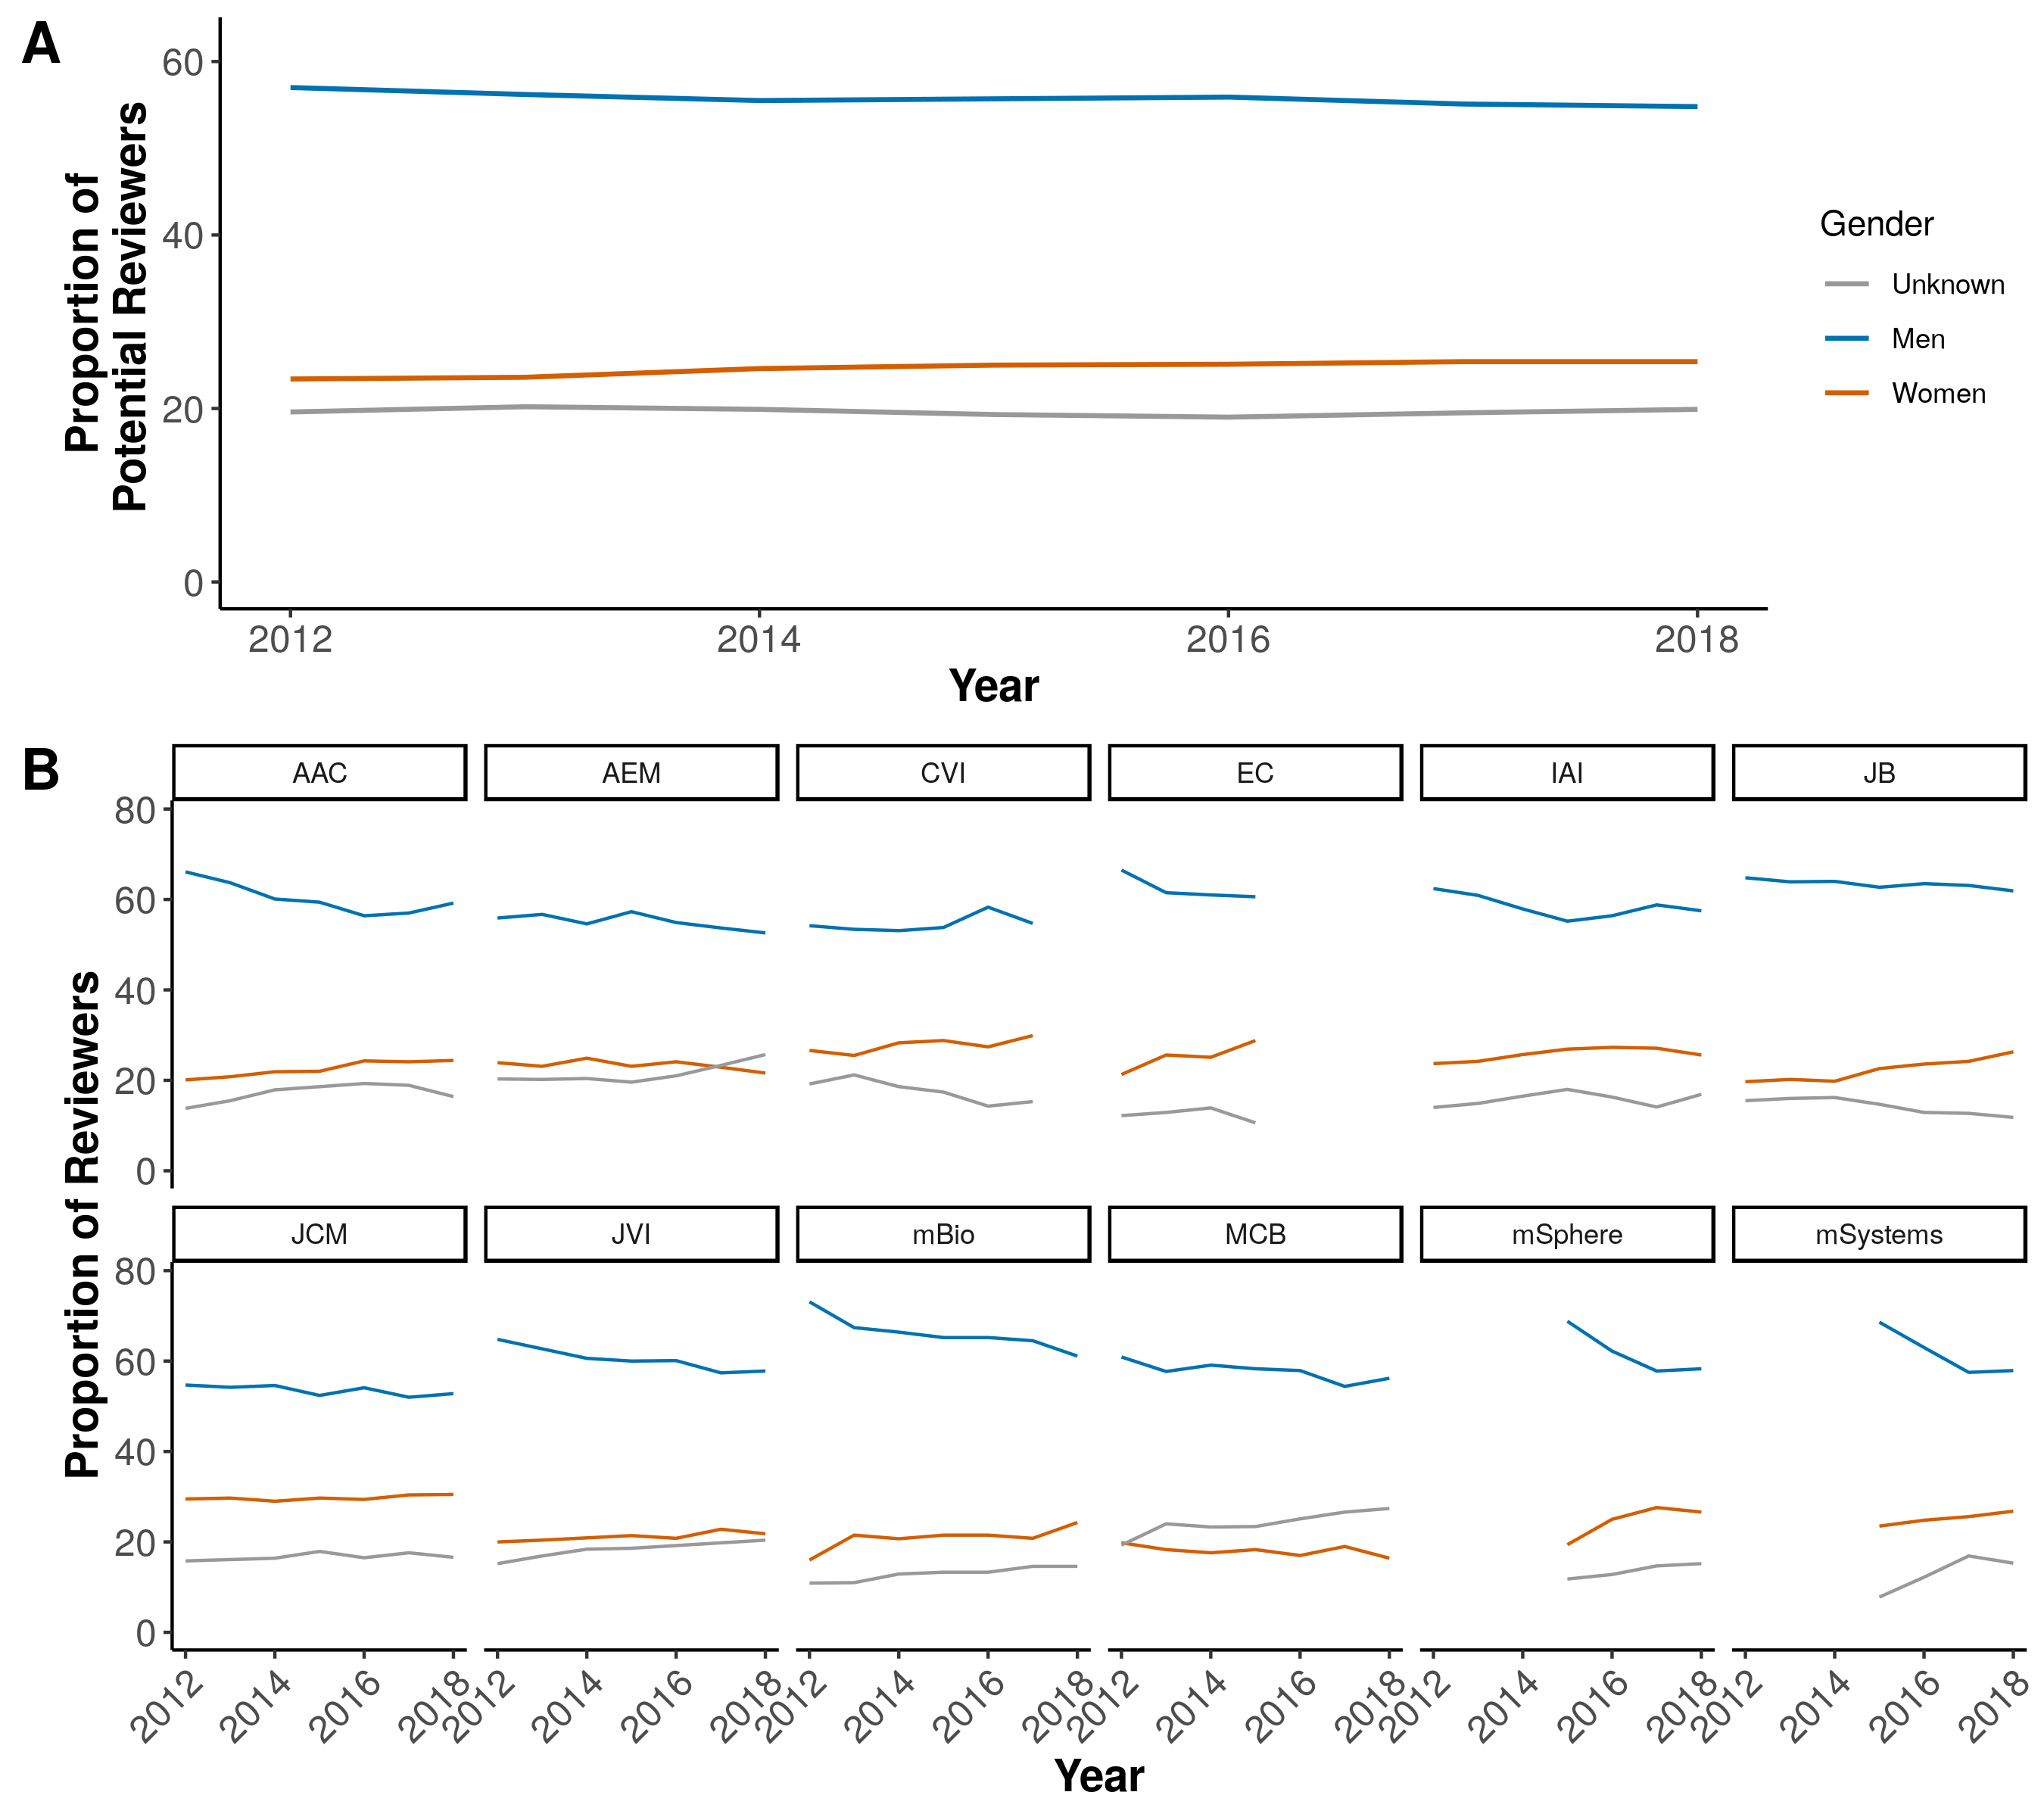
\includegraphics{Figure_S2.png} Figure S2. The proportion of (A)
potential reviewers at all ASM journals combined, (B) reviewers at each
ASM journal.

\newpage

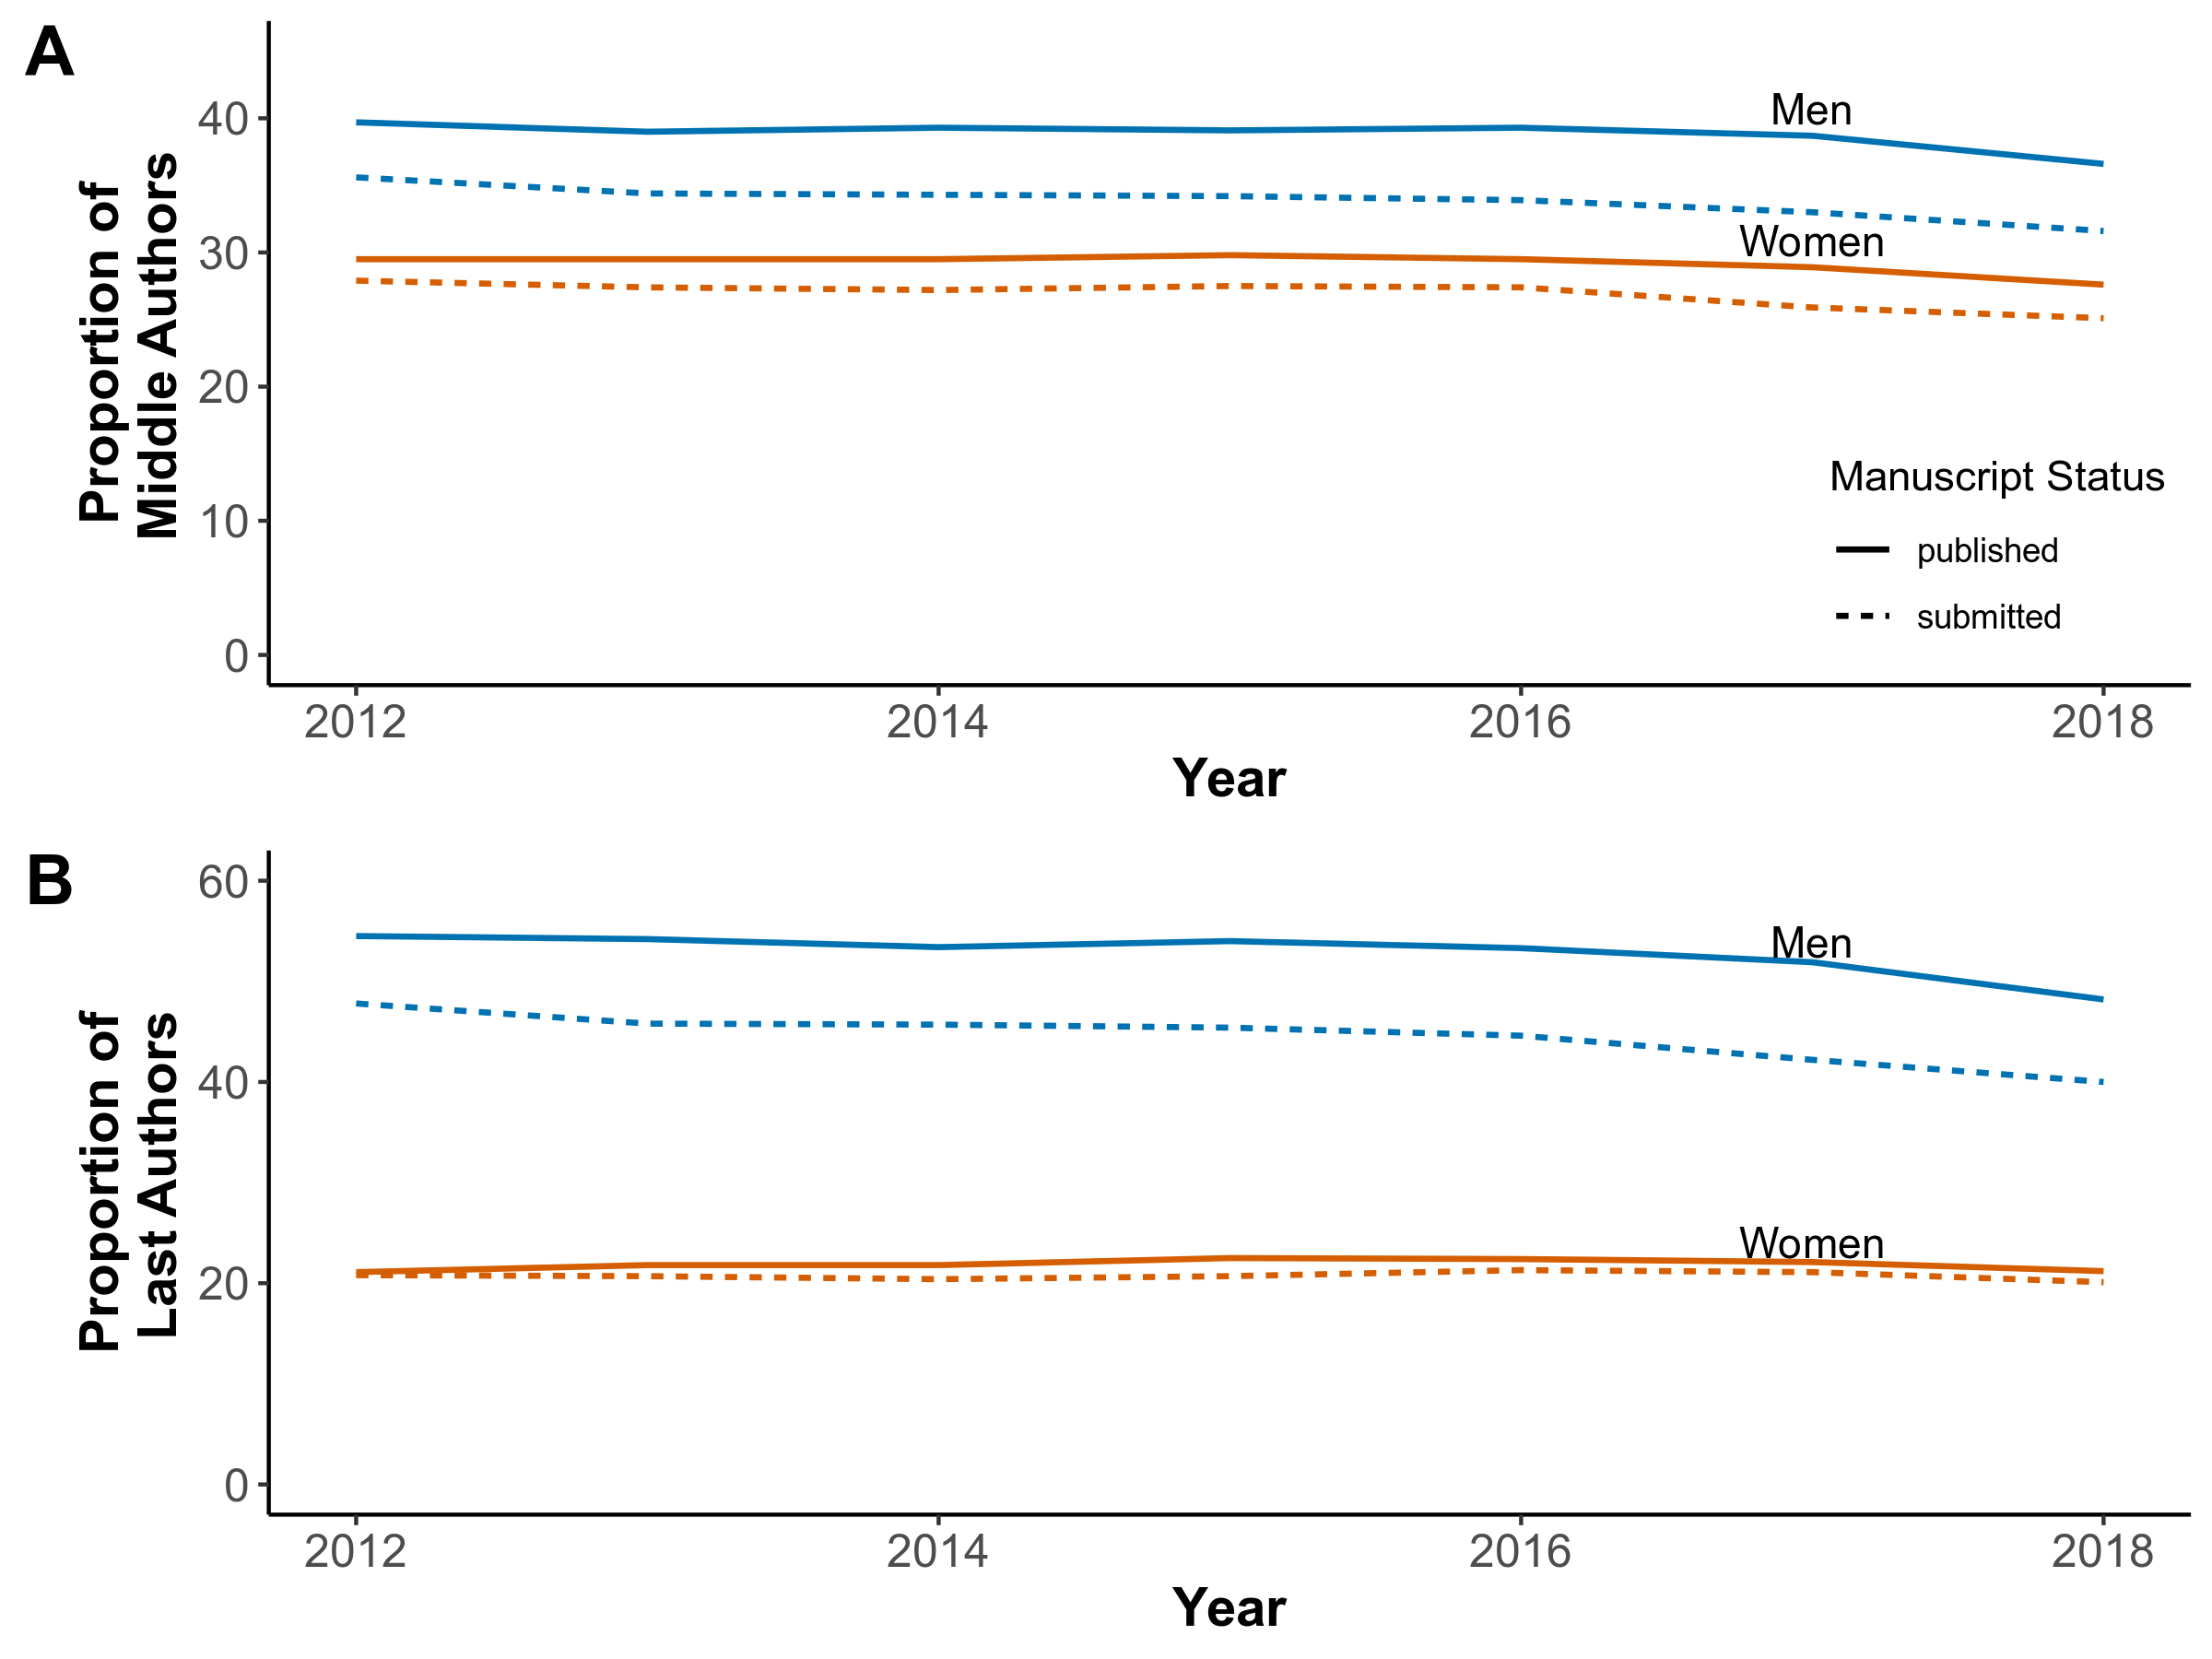
\includegraphics{Figure_S3.png} Figure S3. The proportion of all
submitted (dashed line) and published (solid line) (A) middle and (B)
last authors by gender at each ASM journal.

\newpage

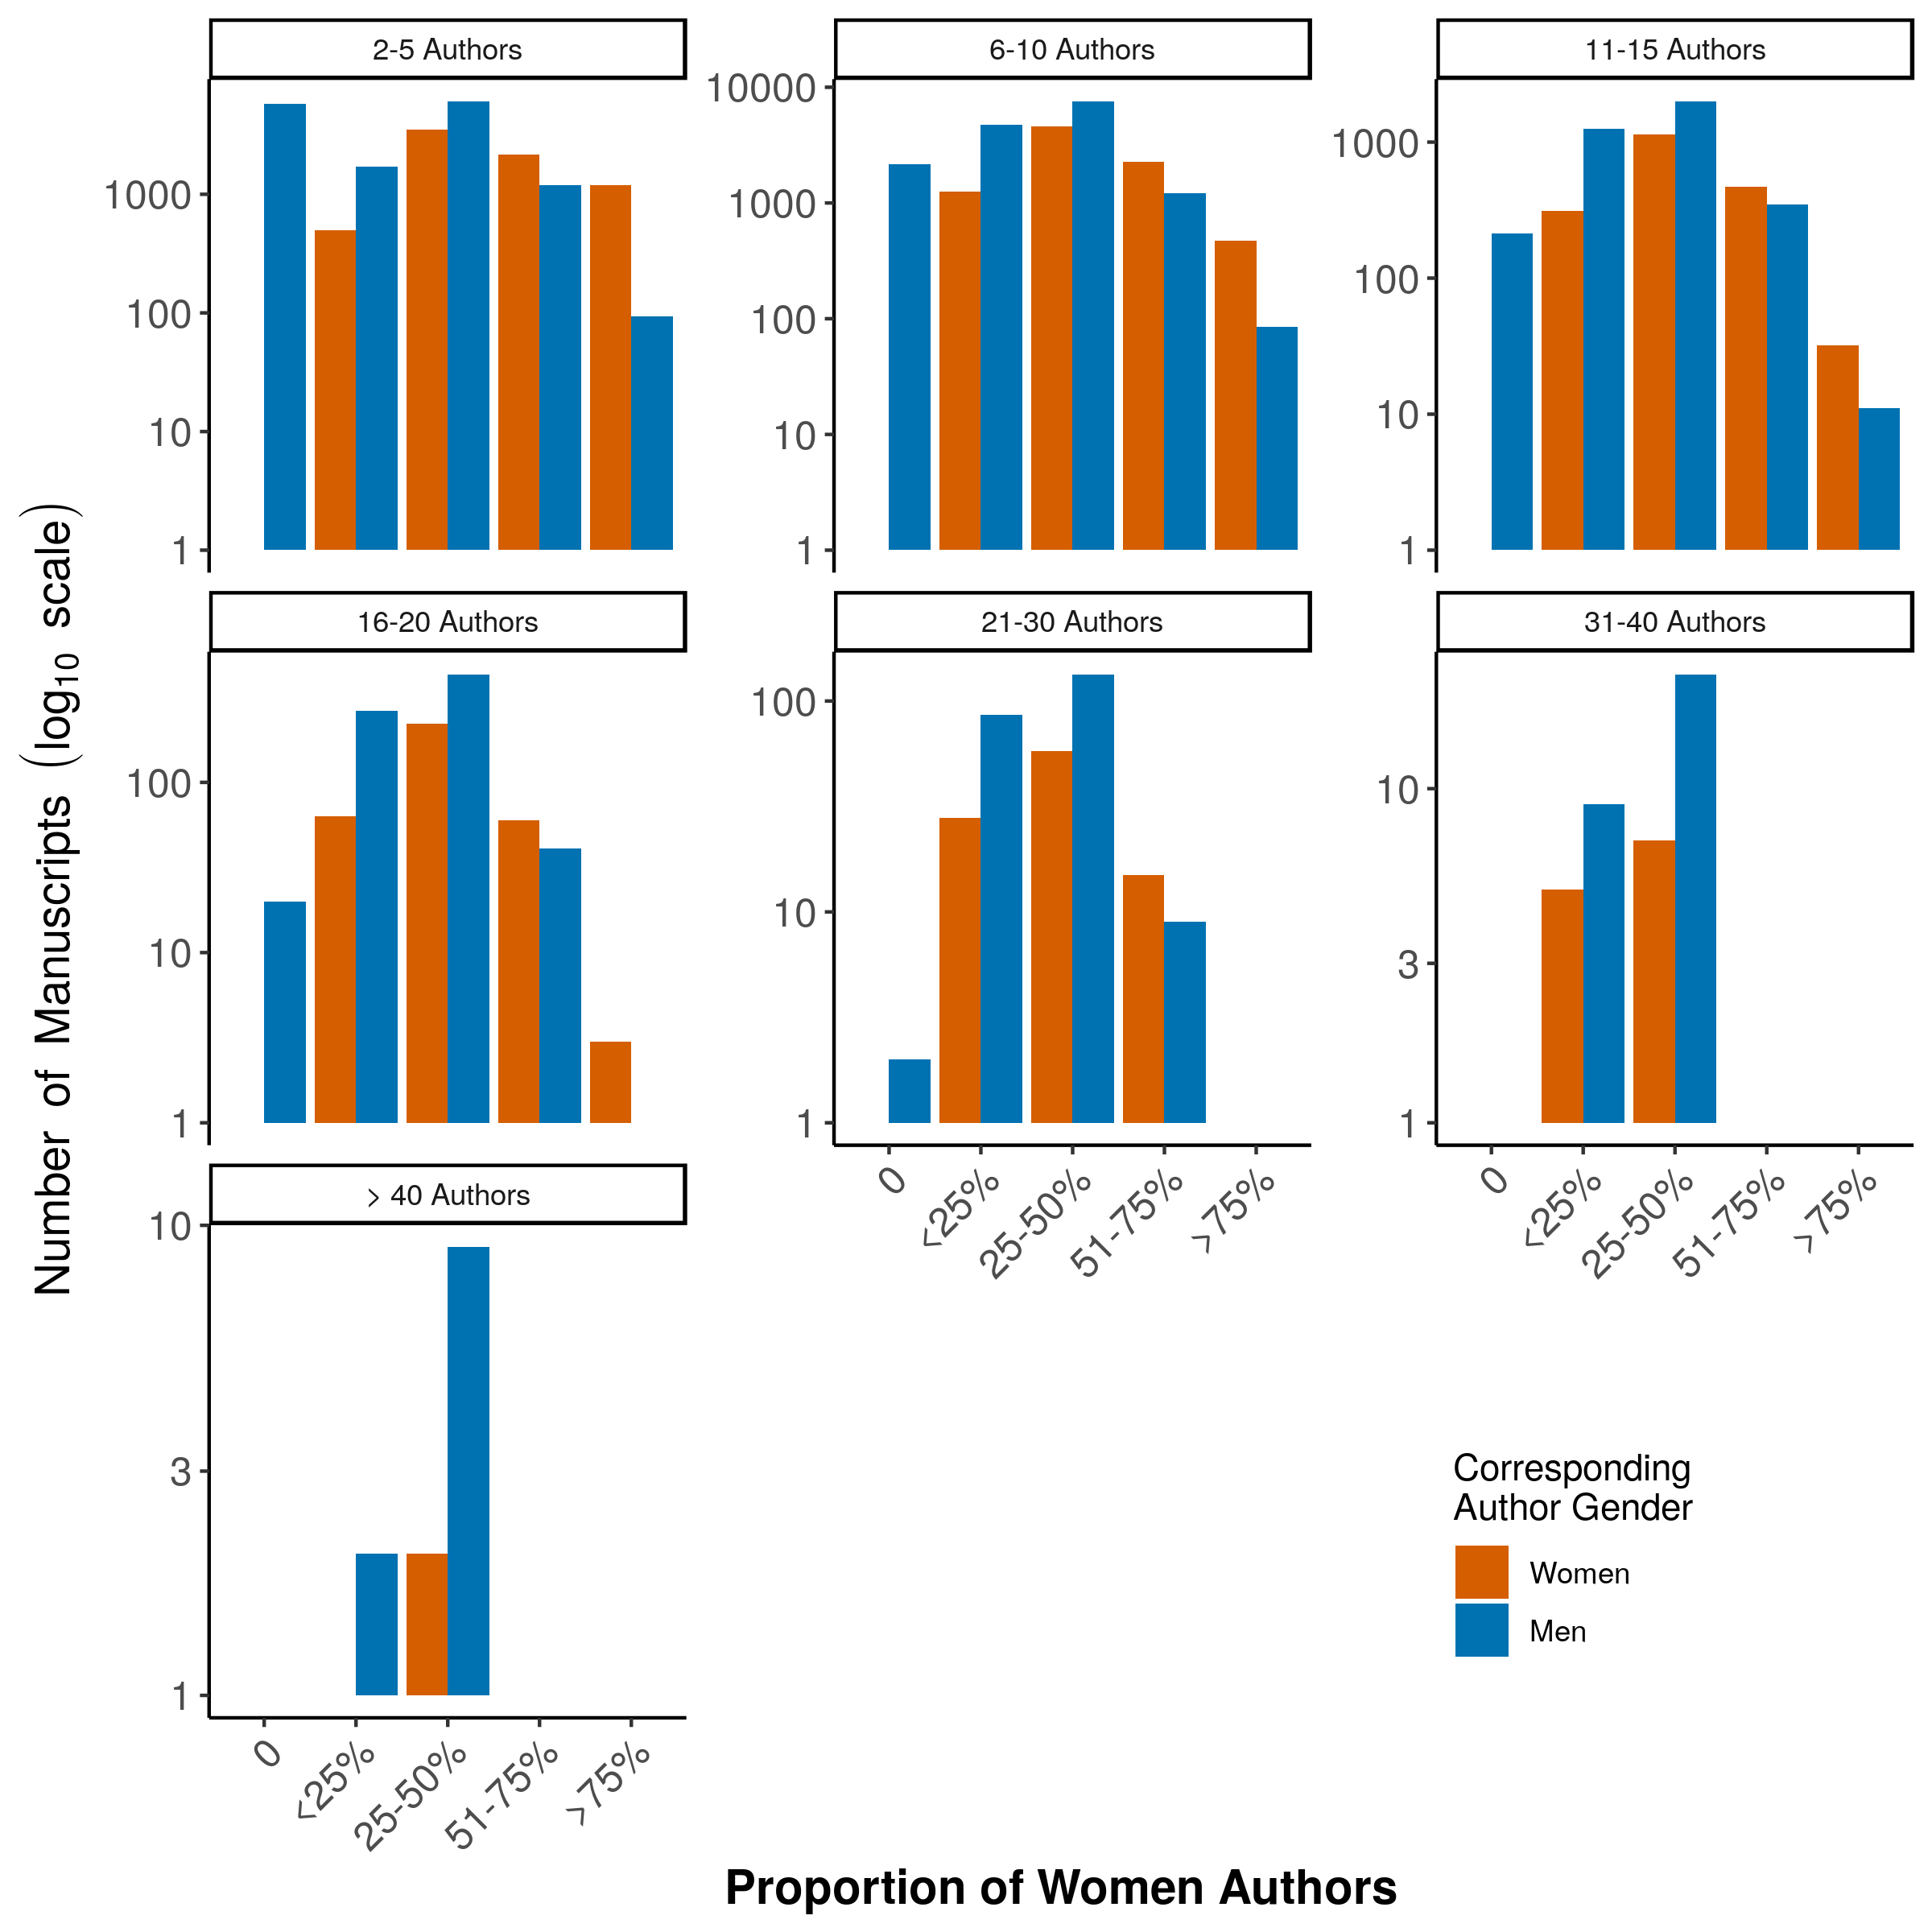
\includegraphics{Figure_S4.png} Figure S4. The proportion of women
authors on submitted manuscripts according to the number of authors and
the gender of the corresponding author. Y axis indicates the total
number of manuscripts on a log\textsubscript{10} scale.

\newpage

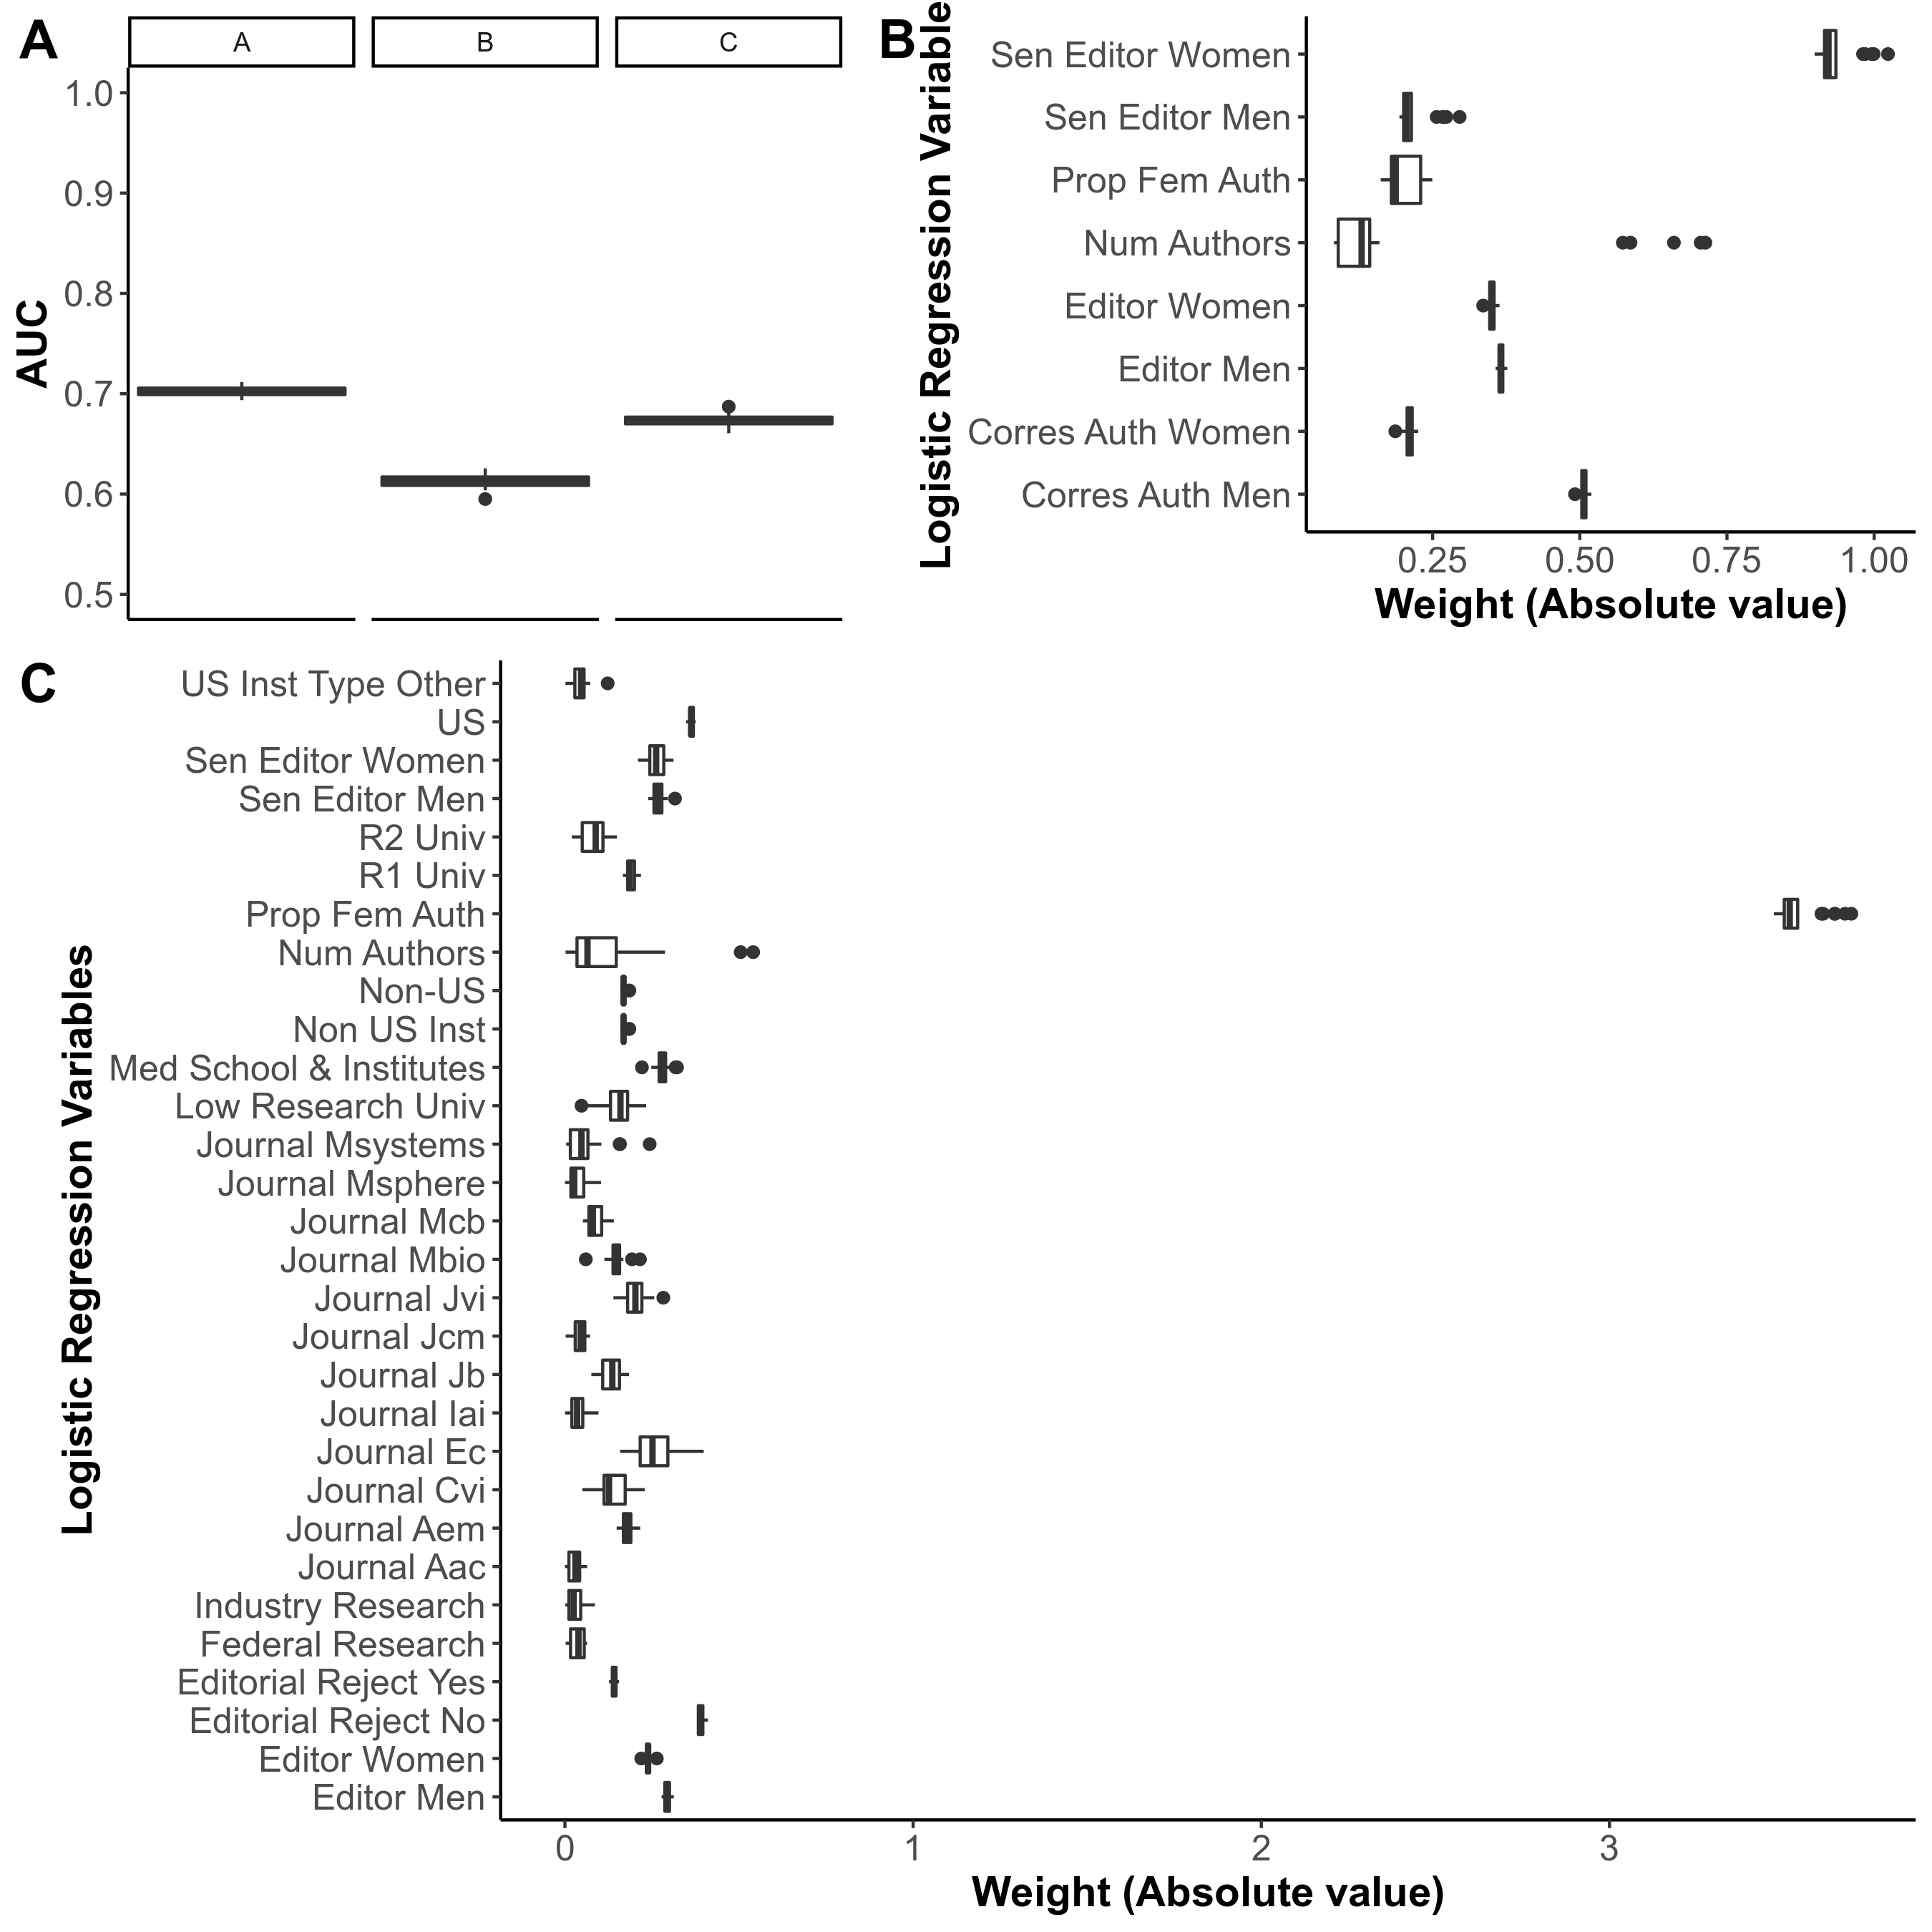
\includegraphics{Figure_S5.png} Figure S5. Comparison of time to final
decision and impact by gender. The number of days (A) between when a
manuscript is initially submitted and finally published or (B) that a
manuscript spends in the ASM peer review system.

\newpage

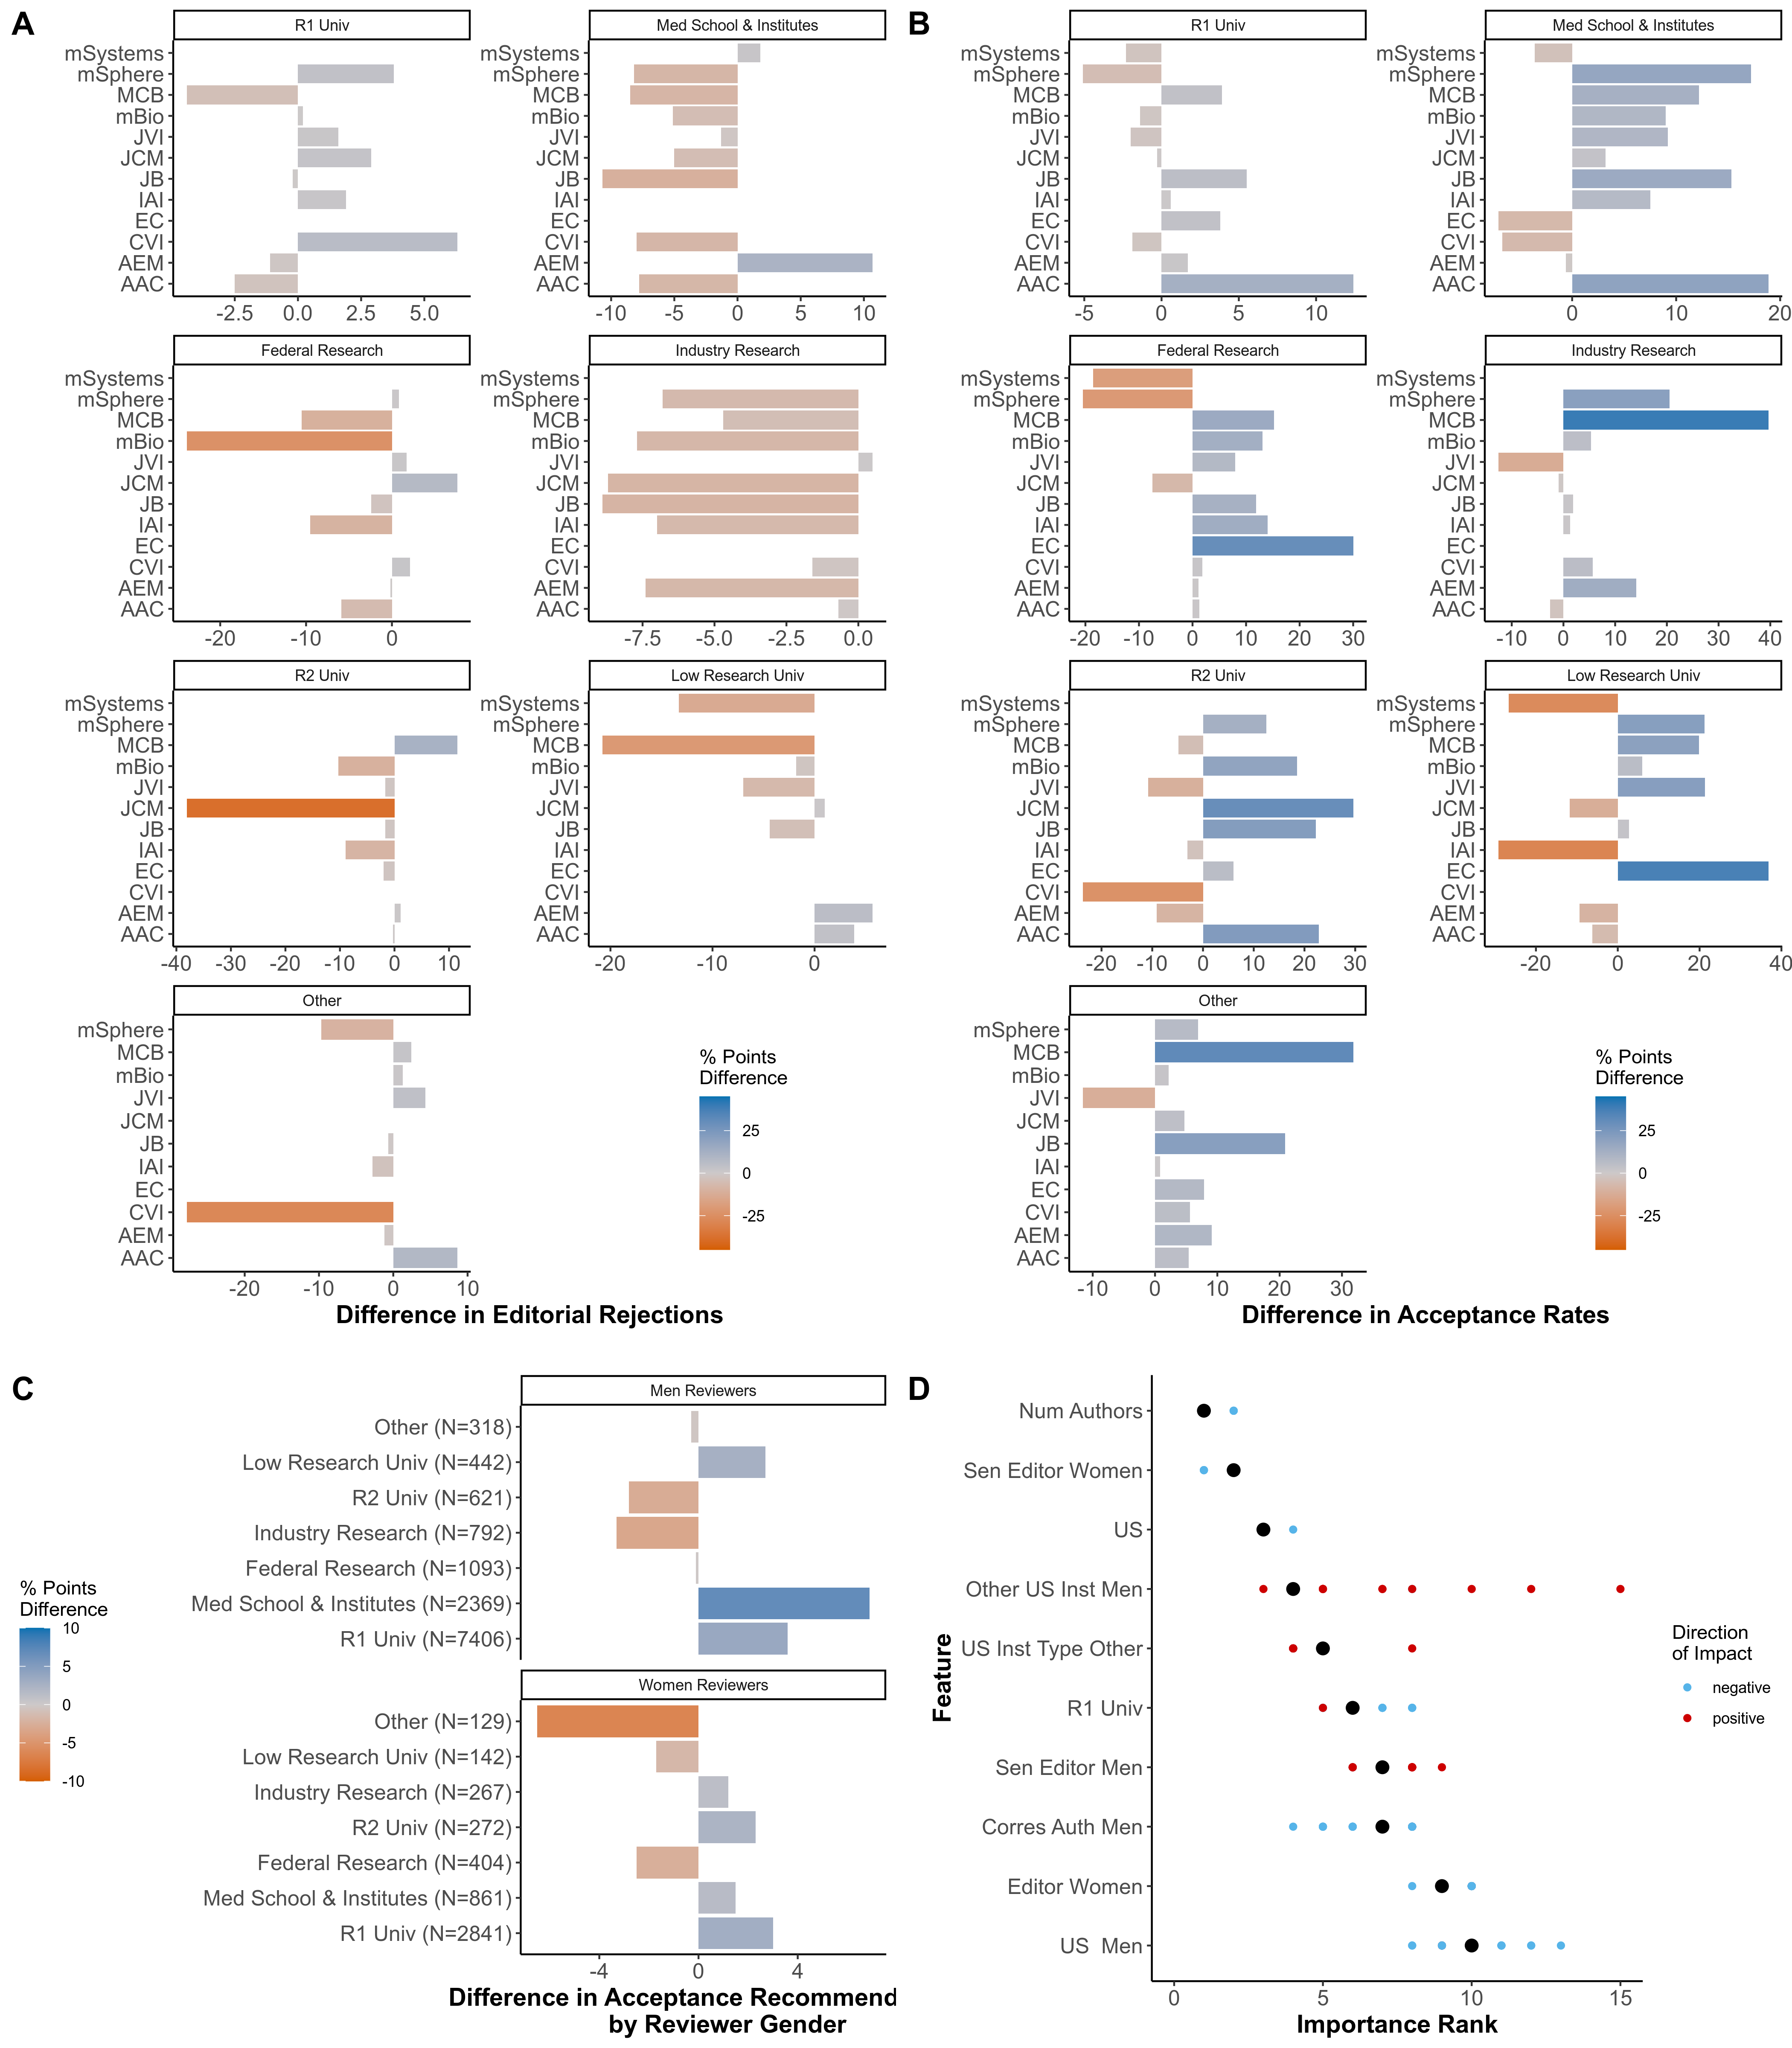
\includegraphics{Figure_S6.png} Figure S6. Difference in A) editorial
rejection and B) acceptance rates by journal and institution type. C)
Difference in review recommendations by reviewer gender and author
institution type. D) Median importance (black dot) of features affecting
editorial rejections, and their range. Color of smaller dots (N=25)
indicate the direction of the impact.

\newpage

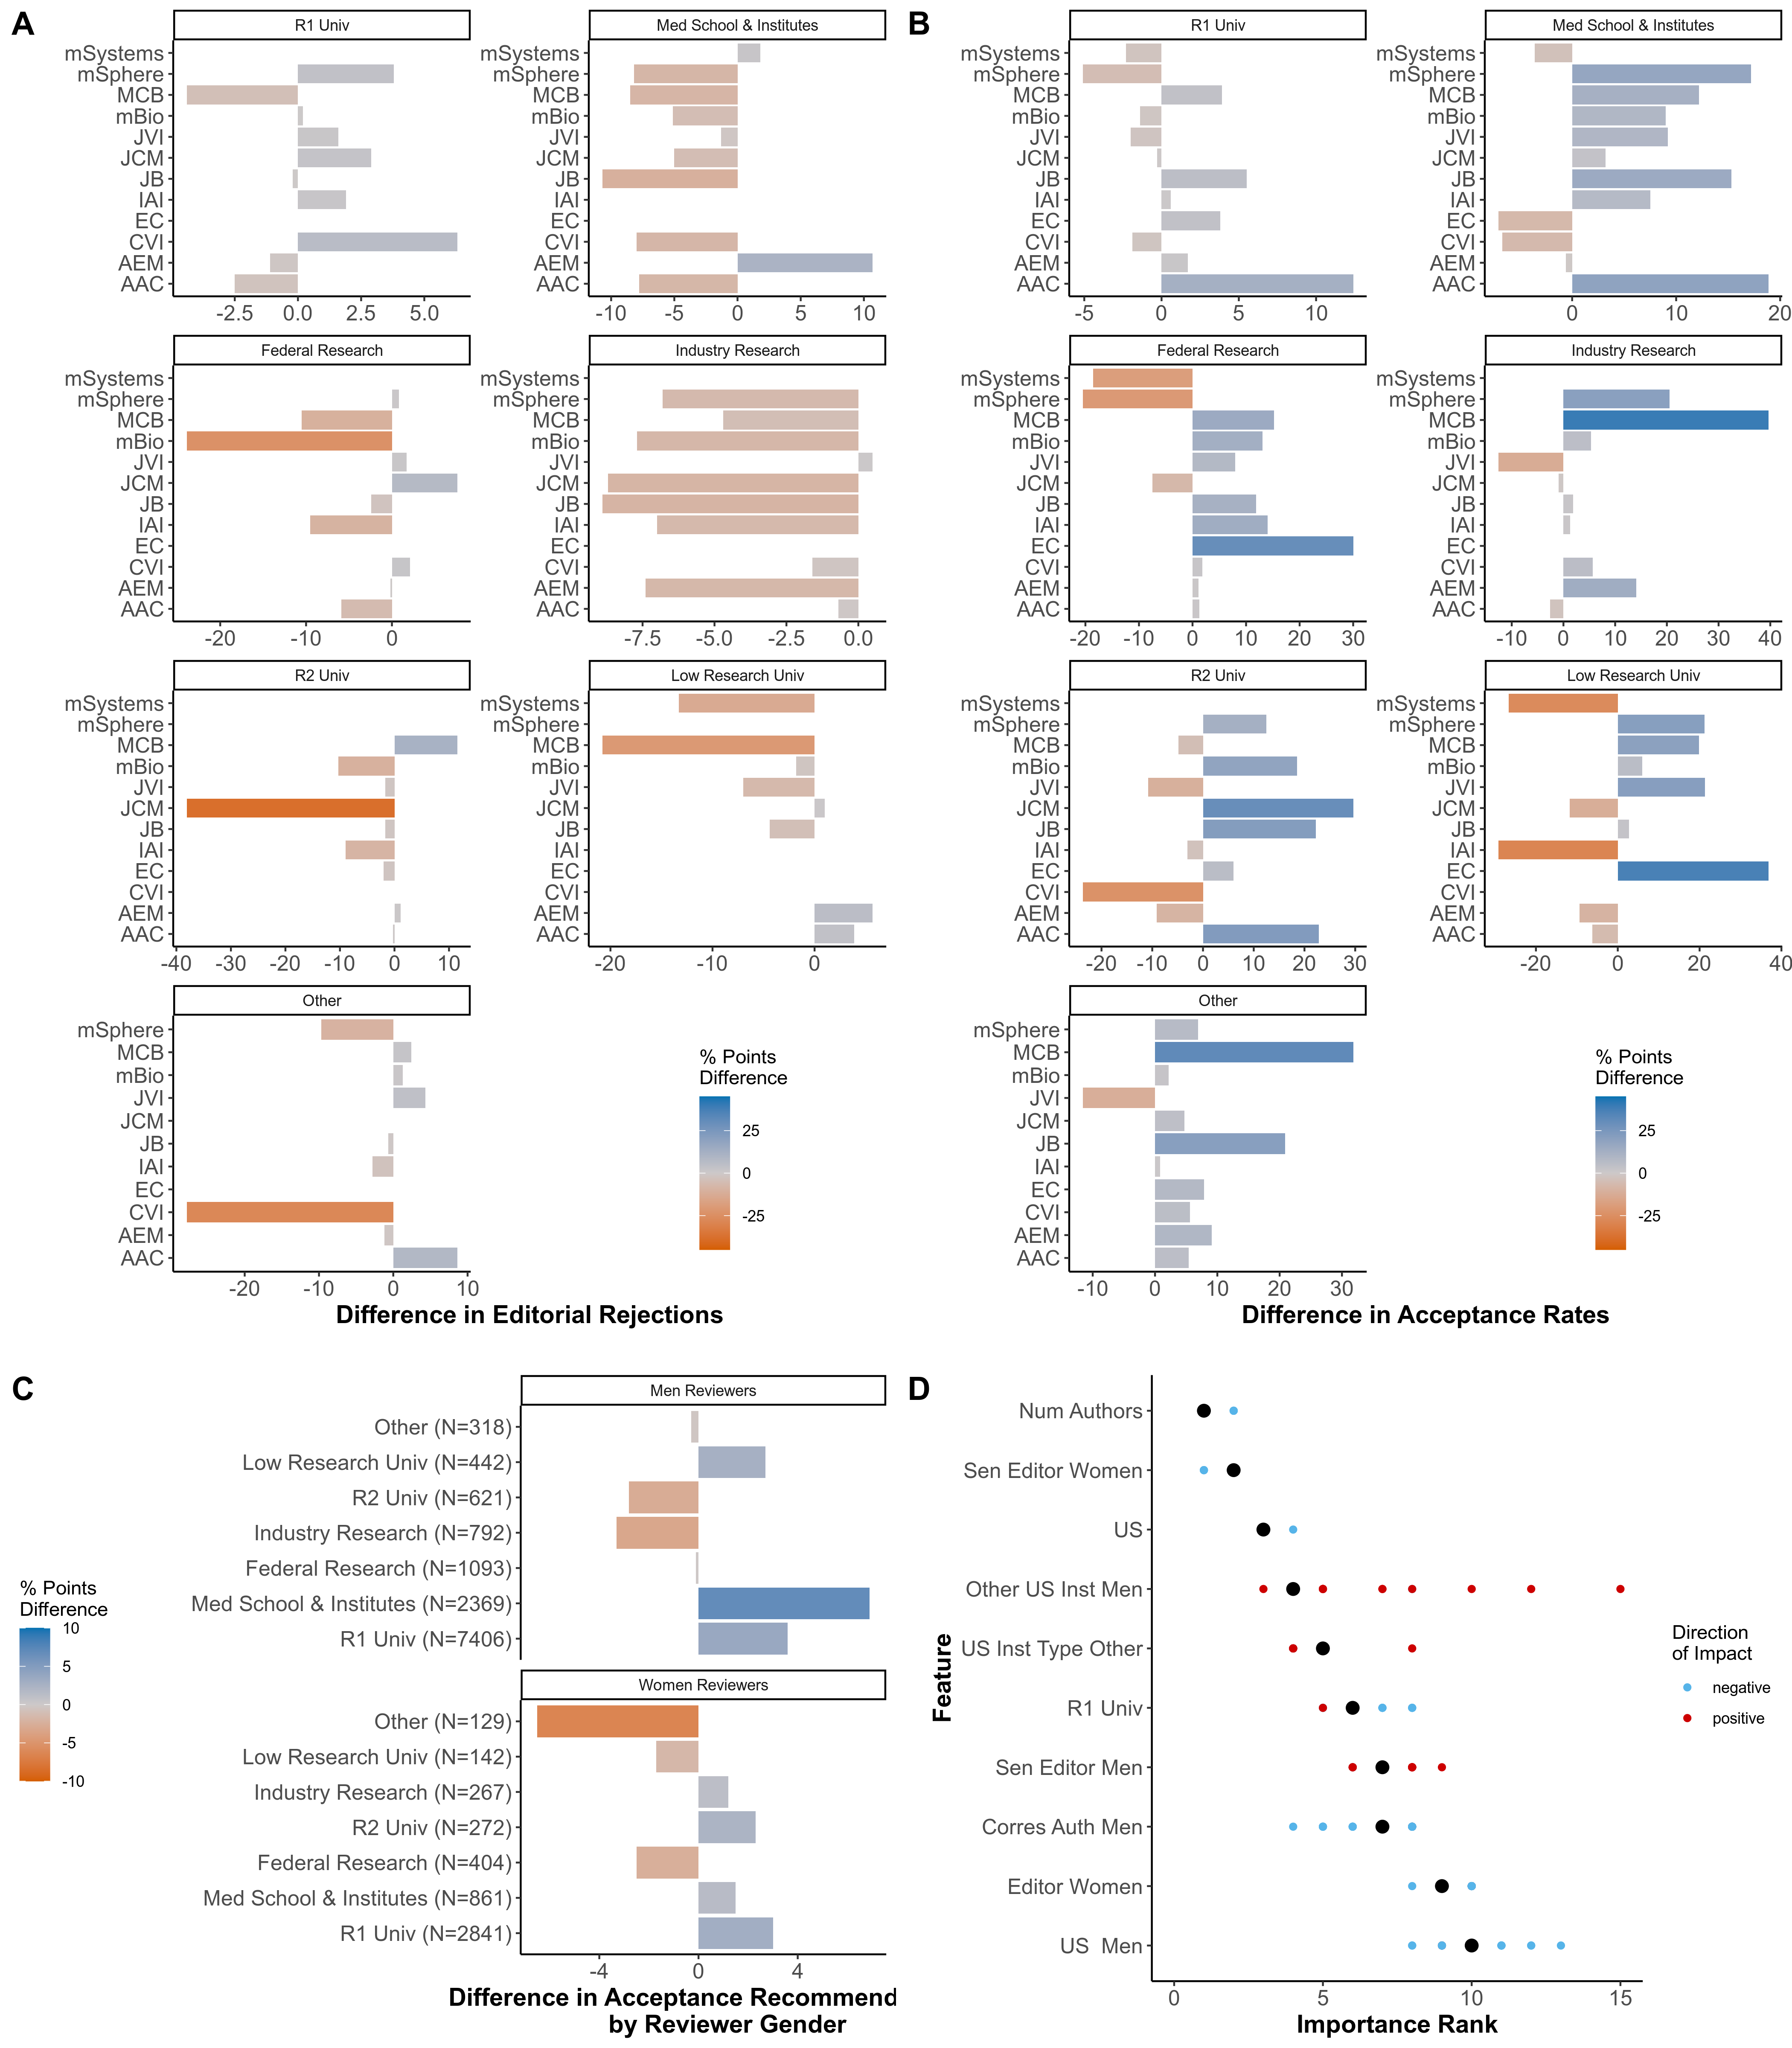
\includegraphics{Figure_S7.png} Figure S7. Difference in editorial
rejections and rejections after review by corresponding author gender
and manuscript category at (A) AAC, (B) AEM, (C) IAI, (D) JCM, and (E)
JVI. In parentheses: N = the number of manuscripts submitted.

\newpage

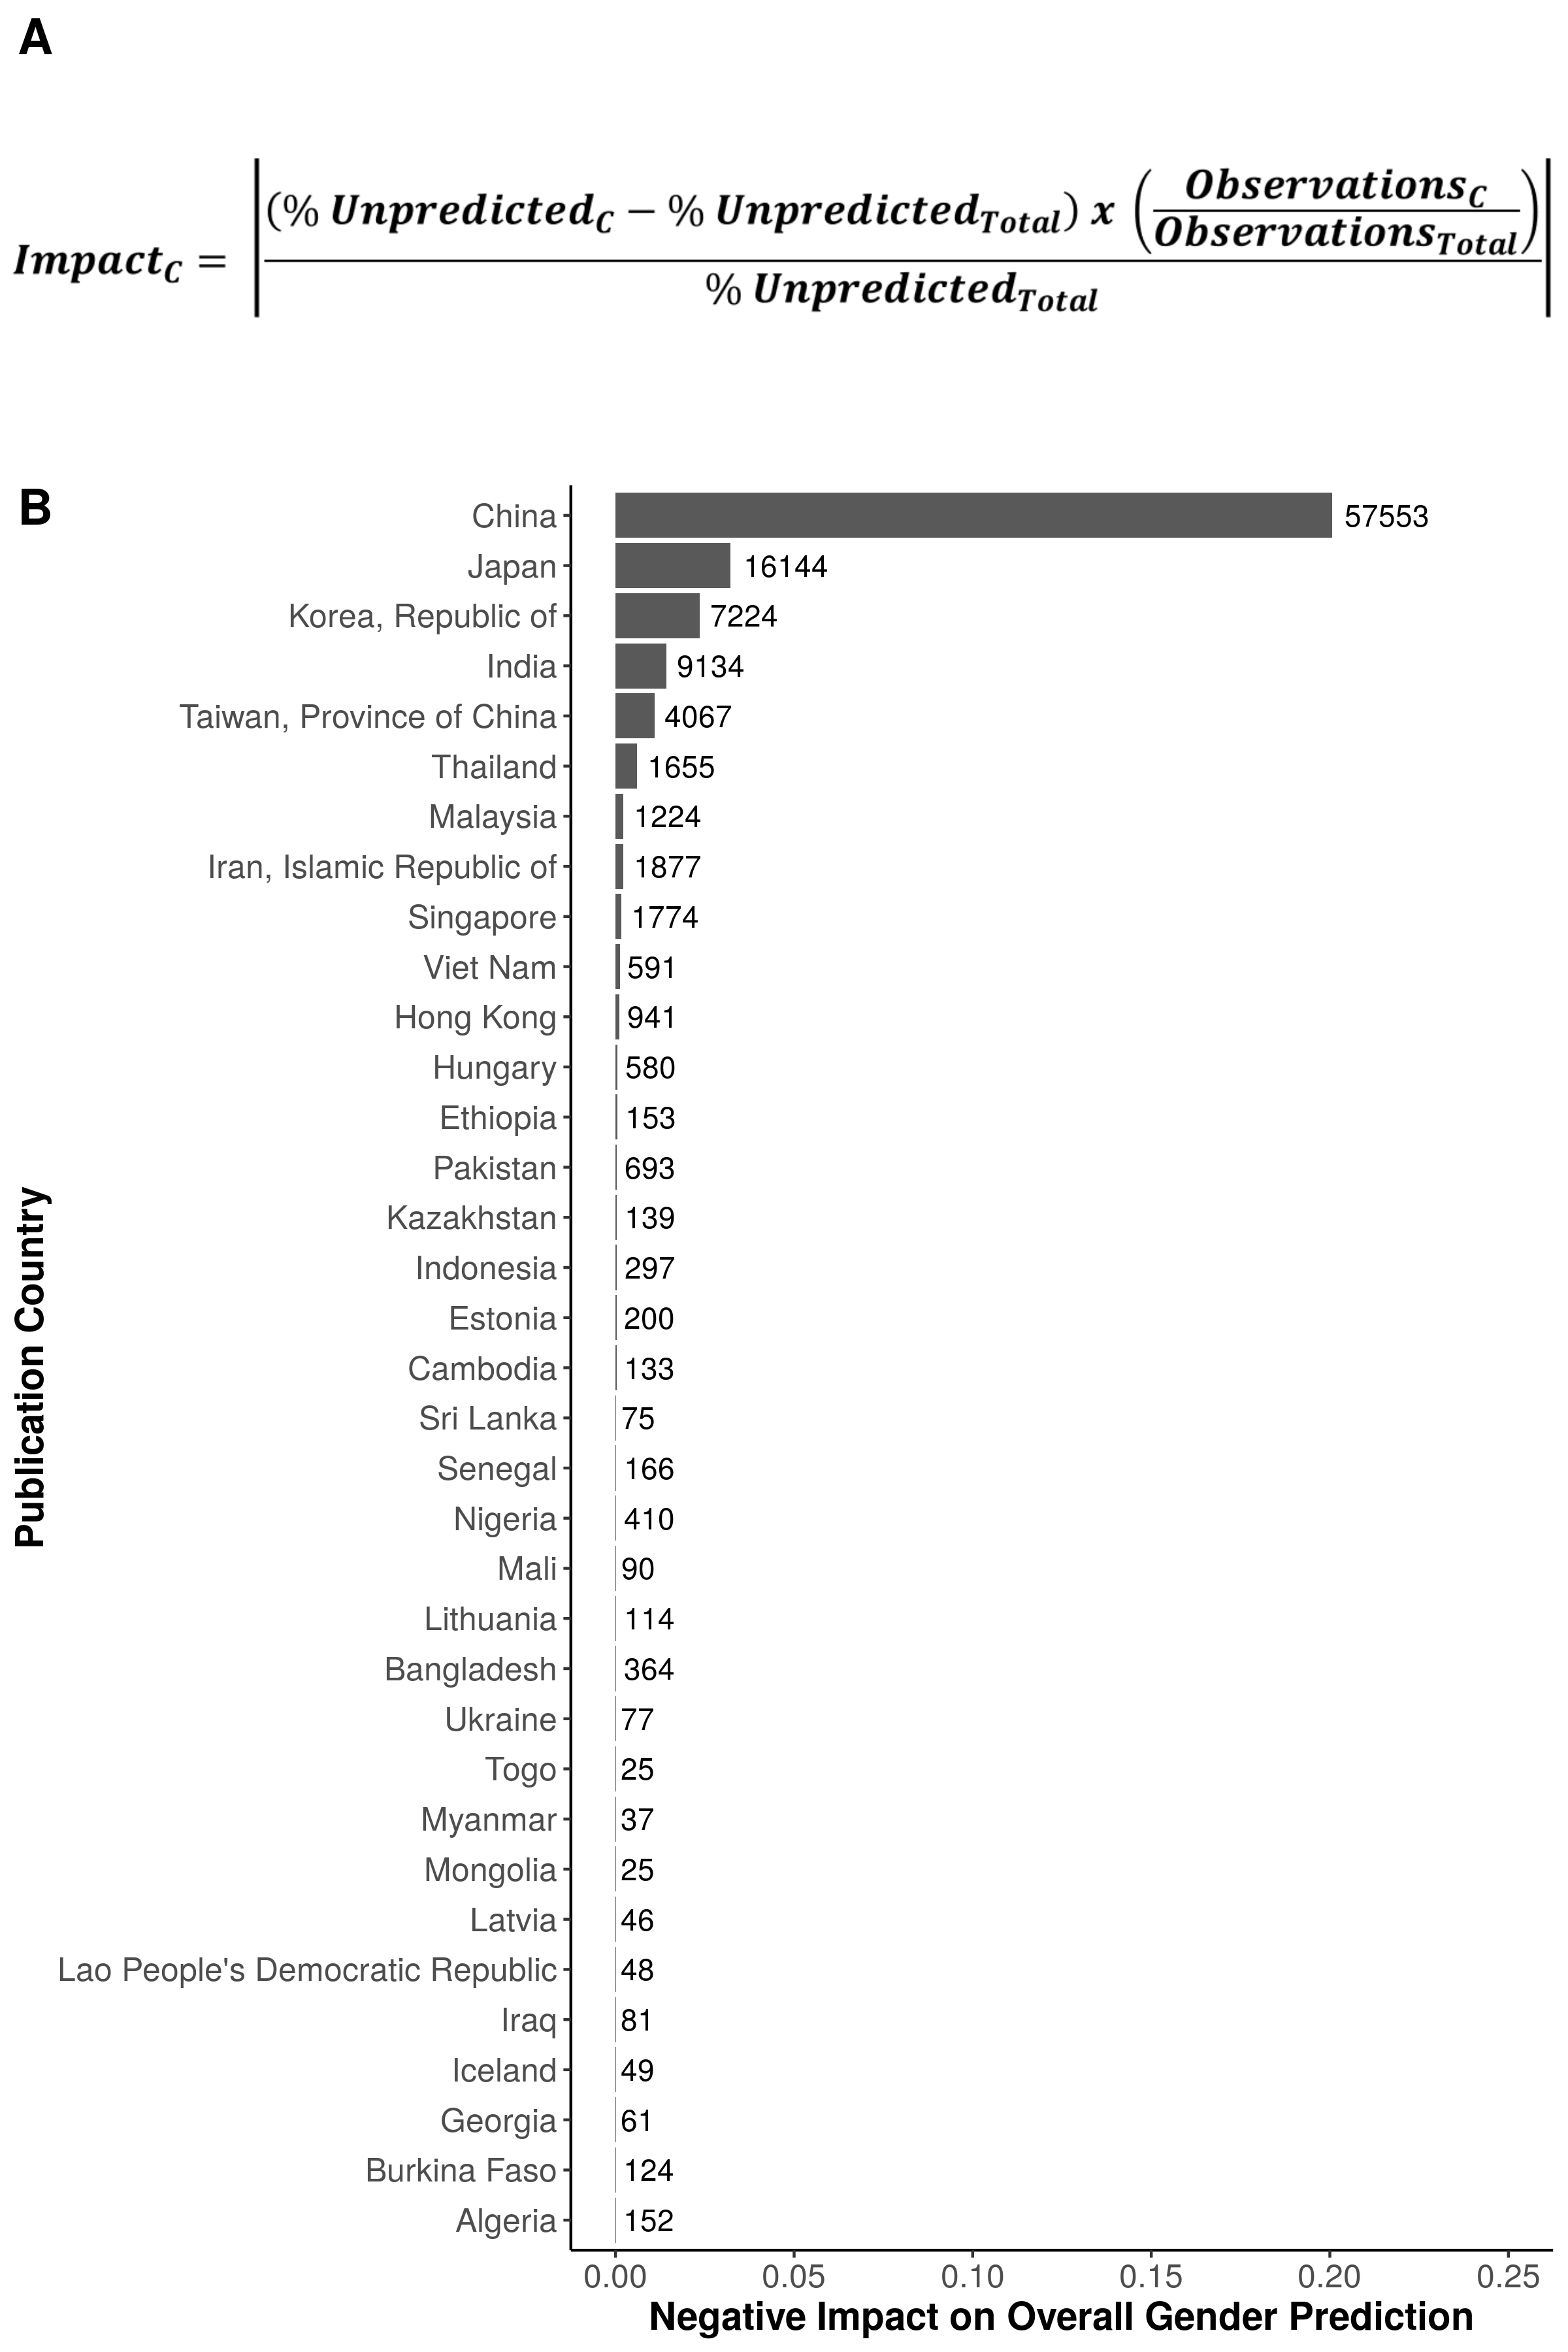
\includegraphics{Figure_S8.png} Figure S8. (A) Equation for calculating
negative bias by genderize algorithm. C indicates a country. (B) The
negative impact of each country on the overall gender inference of the
full data-set. Number to the right of each column is the total number of
names associated with that country.


\end{document}
